% Using KOMA Script document style
% Font size setting and
% option to skip empty lines as new paragraphs
\documentclass[10pt,a4paper]{article}
\usepackage{silence}
\WarningFilter{latex}{Command}
% Packages without Options
\usepackage{
	mathtools,
	array,
	amsfonts,
	amssymb,
	geometry,
	enumitem,
	venndiagram,
	booktabs,
	tikz,
	interval,
	makecell,
	textcomp,
	gensymb,
	float,
	pgfkeys,
	pgfplots,
	wrapfig,
	lipsum,
	karnaugh-map,
	footnote,
	tablefootnote,
	xcolor,
	longtable,
	subcaption,
	algorithm,
	algpseudocode,
	pdfpages,
    nicematrix,
    sectsty,
    titlecaps,
	listings,
	minted,
	wrapfig,
}

\definecolor{mintedbackground}{rgb}{0.97,0.97,0.97}

\setminted[cpp]{
bgcolor=mintedbackground,
    linenos=true,
    breaklines=true,}

\setminted[python]{
bgcolor=mintedbackground,
    linenos=true,
    breaklines=true,}
    
% Enforce title case for section
% \allsectionsfont{\titlecap}

% \lstset{basicstyle=\footnotesize\ttfamily,breaklines=true}

\linespread{1.5}

% Packages with Options
\usepackage[british]{babel} 
\usepackage[framemethod=tikz]{mdframed}
\usepackage[colorlinks,linkcolor=cyan, citecolor=cyan, urlcolor=cyan]{hyperref}
\usepackage[labelfont=bf,textfont=it,labelsep=period]{caption}
\usepackage[RPvoltages]{circuitikz}

% Package: Interval
% Sets the style of mathematical intervals
\intervalconfig{
soft open fences, separator symbol=,,
}

% Package: Geometry
% Sets the page margins
\geometry{
    a4paper,
    left=32mm,
    right=22mm,
    top=22mm,
    }
	
% Creates a proper caption name for algorithms
\newcommand{\algorithmautorefname}{Algorithm}
\newcommand{\listingautorefname}{Listing}
\algrenewcommand{\algorithmiccomment}[1]{\texttt{// #1} }
% Creates a numbered environment for Theorems
\newtheorem{theorem}{Theorem}

% Redefine the implication arrow to be a simple, thin arrow instead of the default, thick arrow
\renewcommand{\implies}{\rightarrow}

% Create a new command for the set complement to make my logical statements easier to read
\newcommand{\compl}{\overline}

% Creates commands for combinatorics nCr and nPr
\newcommand{\nCr}[2]{\,_{#1}C_{#2}} % nCr
\newcommand{\nPr}[2]{\,_{#1}P_{#2}} % nPr

% Package: tikz
% Loads libraries for drawing automata, 
\usetikzlibrary{automata,positioning,shadows,arrows, shapes.gates.logic.US, calc}

% Creates a command to create a button shape
\newcommand*\keystroke[1]{%
  \tikz[baseline= (key.base)]
    \node[%
      draw,
      fill=white,
      drop shadow={shadow xshift=0.25ex,shadow yshift=-0.25ex,fill=black,opacity=0.75},
      rectangle,
      rounded corners=2pt,
      inner sep=1pt,
      line width=0.5pt,
      font=\scriptsize\sffamily
    ] (key) {#1\strut};
}

% Package: pgfplot
% Sets the global options for PGF Plots
\pgfplotsset{compat=newest}

% Package: tikz
% Flowchart Shapes
\tikzstyle{startstop} = [rectangle, rounded corners, minimum width=3cm, minimum height=1cm,text centered, draw=black, fill=red!30]
\tikzstyle{io} = [trapezium, trapezium left angle=70, trapezium right angle=110, minimum width=3cm, minimum height=1cm, text centered, draw=black, fill=blue!30]
\tikzstyle{process} = [rectangle, minimum width=3cm, minimum height=1cm, text centered, draw=black, fill=orange!30]
\tikzstyle{decision} = [diamond, minimum width=3cm, minimum height=1cm, text centered, draw=black, fill=green!30]
\tikzstyle{arrow} = [thick,->,>=stealth]

% Disable Minted syntax error highlights (red boxes)
\AtBeginEnvironment{minted}{%
  \renewcommand{\fcolorbox}[4][]{#4}} %Adjust this based on where your Summary is stored
\title{CM2020: Agile Software Projects \\ Final Project Report, Group 6 (Tutor Group 1)}
\author{B. Currey, B. Lazaruk, A. Muralidharan, A. Milosevic \& H.C. Ishida}
\begin{document}


\maketitle
\newpage
\tableofcontents
\listoffigures
%\listoftables
% \listofalgorithms
\listoflistings
\newpage
\renewcommand{\subsubsectionautorefname}{section\negthinspace}
\section*{Reference to Rubric}
The table below provides references to the relevant sections where specific grading criteria can be found in this report. A live version of the application is hosted at \url{https://tbd}.

\begin{table}[H]
	\small
	\begin{tabular}{@{}m{10cm}!{\qquad}m{5cm}@{}}
	\toprule
	\textbf{Criteria}                                                & \textbf{Location in Report}     \\ \midrule
	\textbf{Technical}                                               &                                 \\
	Code solves challenges presented in the aims/objectives          &                                 \\
	Iterative Design                                                 &  \Cref{sec:iterative_design}, \Cref{sec:cycle1}   \\
	Approach is fit for purpose without drastic oversights           &  \Cref{sec:techapproach}       \\
	Elegance/aesthetics/readability of code                          &  \Cref{sec:code}               \\
	Sensible approach to structure                                   &  \Cref{sec:files}              \\
	Evidence of collaboration and team work                          &  \Cref{sec:roles}             \\
	Evidence of milestones and reflective updates                    &  \Cref{sec:milestones_updates}  \\
	Difficulty of technical challenge                                &  \Cref{sec:techdiff}            \\
	Novelty of technical challenge                                   &  \Cref{sec:techdiff}     \\
	\textbf{Testing}                                                 &                             \\
	All parts of the system working                                  &   \Cref{sec:autotest}    \\
	UI evaluation                                                    &   \Cref{sec:uieval}    \\
	Well documented tests                                            &   \Cref{sec:autotest}      \\
	Effective error handling                                         &                             \\
	Systematic testing regime including design of appropriate test cases & \Cref{sec:autotest}    \\
	Justification of testing methods                                 &    \Cref{sec:testing}    \\
	User evaluation involving representative stakeholders formative  &     \Cref{sec:formative}    \\
	User evaluation involving representative stakeholders summative  &    \Cref{sec:summative}  \\
	\textbf{Report}                                               &                                \\
	Good introduction and fair discussion of literature              &     \Cref{sec:introlit}   \\
	Clear statement of problem and effective problem analysis        &     \Cref{sec:prob}   \\
	Clear structure                                                  &     see Table of Contents      \\
	Justification of design decisions                                &     \Cref{sec:justif}   \\
	Good argumentation and justification of claims/problem analysis  &     \Cref{sec:prob}     \\
	Clear documentation and user guide                               &     \Cref{sec:guide}      \\
	Sufficient and appropriate references, and good citing method    &                             \\
	Good layout and formatting, especially of tables, figures, formulae and code examples          &  \\
	Well written with systematic analysis                            &                             \\
	Insightful discussion of results                                 &                             \\
	Evaluation of own work in relation to original proposal and plan &                             \\
	Conclusion and discussion of future work                         &                             \\ \bottomrule
	\end{tabular}
\end{table}


\section{Background, Aims and Objectives}

\subsection{Introduction and Literature}\label{sec:introlit}
This project aims to develop a grades leaderboard for students to share grades. Before diving further into the context and objective of our project, we will briefly describe the most important literature used in developing this work.

The academic foundations of this project are drawn from \cite{interaction_design} as a primary source for design methodology. This text describes the double diamond design approach, which was at the heart or our approach. It allowed us to widen our scope at the start of the project, yet letting us quickly select a high-potential idea for further development. We critically considered this approach alongside others, as will be discussed further in \cref{sec:iterative_design}. 
Our testing methodology during development was based on the UMUX-Lite whitepaper \cite{lewis}, which enabled collecting user feedback on the user experience with little effort on behalf of test subjects, yet still allowing us to assemble a quantiative view on user feedback during summative assessment, as described further in \cref{sec:uieval}.
Our user interface has been largely designed using princples from \cite{mckay_2013}, which outlines effective communication of functionality and usability of applications. We used this extensively in designing buttons, UI elements and descriptions as outlined in \cref{sec:justif}.

\subsection{Context and Problem Statement} \label{sec:prob}
Motivation to study is a scarce resource for university students and one that can easily get depleted. Today’s connected and highly technological environment provides the opportunity to use gamification to increase motivation and provide to students and to the educational institutions that they partake in \cite{garciacabot_measuring_2020} \cite{lister_gamification:_2015}. 

In addition, students with a competitive mindset might draw additional motivation from the ability to compare themselves to peers and identify opportunities to improve their own skills.

Every module in a degree program is different and may require a tailored strategy for studying. Reflecting on a completed module provides “hindsight 20/20” notes on what worked well and what can be improved. In a collaborative environment however, students are not limited to their own experiences - they can benefit from the wisdom and experience of fellow students.


The \textbf{problem} that we aim to solve is that students normally have no way to easily compare their own grades to those of their peers, and cannot assess if their grade is within an expected range for any given module. For prospective students of a module, it is hard to judge if a certain module usually provides high grades or not, and what effort might be associated with achieving such a grade. For students who have received grades, there is little opportunity to find out whether a received grade is reasonable given the self-perceived effort and completed coursework.

\subsection{Opportunity}

We aim to motivate the students to be their best selves and adopt the life-long growth mindset.

Our review of academic literature found evidence for positive effect of use of leaderboards on student motivation \cite{chiu_effects_2017} \cite{jia_designing_2017}.

To realise this long-term aim, we propose development of a \textbf{grades leaderboard} that allows students to share and compare grades, while managing their own grades for a given university program. 

This report outlines how we decided to pursue this opportunity, what we aim to achieve, how we aim to achieve it and how we will measure outcomes.

\subsection{Goals}
With this project, we are pursuing the following goals. Details of critical success factors that measure achievement of these goals are provided in section 6.

\paragraph{Business Goals}
\begin{itemize}
    \item Launch a grades leaderboard in one program with real students
    \item Gain traction so that the solution becomes an established part of student life
\end{itemize}

\paragraph{Usability Goals}
\begin{itemize}
    \item Make entering and sharing feel extremely fast and frictionless
    \item Make students feel safe in sharing their grades online
\end{itemize}

\paragraph{Technical Goals}
\begin{itemize}
    \item Ensure the security of the platform to ensure integrity of the data provided
    \item Make the application easily accessible as web application
\end{itemize}


\section{Planning and Research}

\subsection{Planning}

We chose an iterative implementation approach that fits multiple cycles of design, development and user testing from the start of the year until submission of the project by mid-March. This approach envisions that based on completed initial requirements analysis by the end of the year, we can start with short, 2-week cycles of developing the solution. This phase will be closer to a Google Design Sprint in which the team spends focused, full days in developing solutions, implementing prototypes and iterating on the product.

Our timeline plan is shown in \cref{fig:gantt} illustrating the cycle-based approach until March of 2021.

\begin{figure}[H]
    \centering
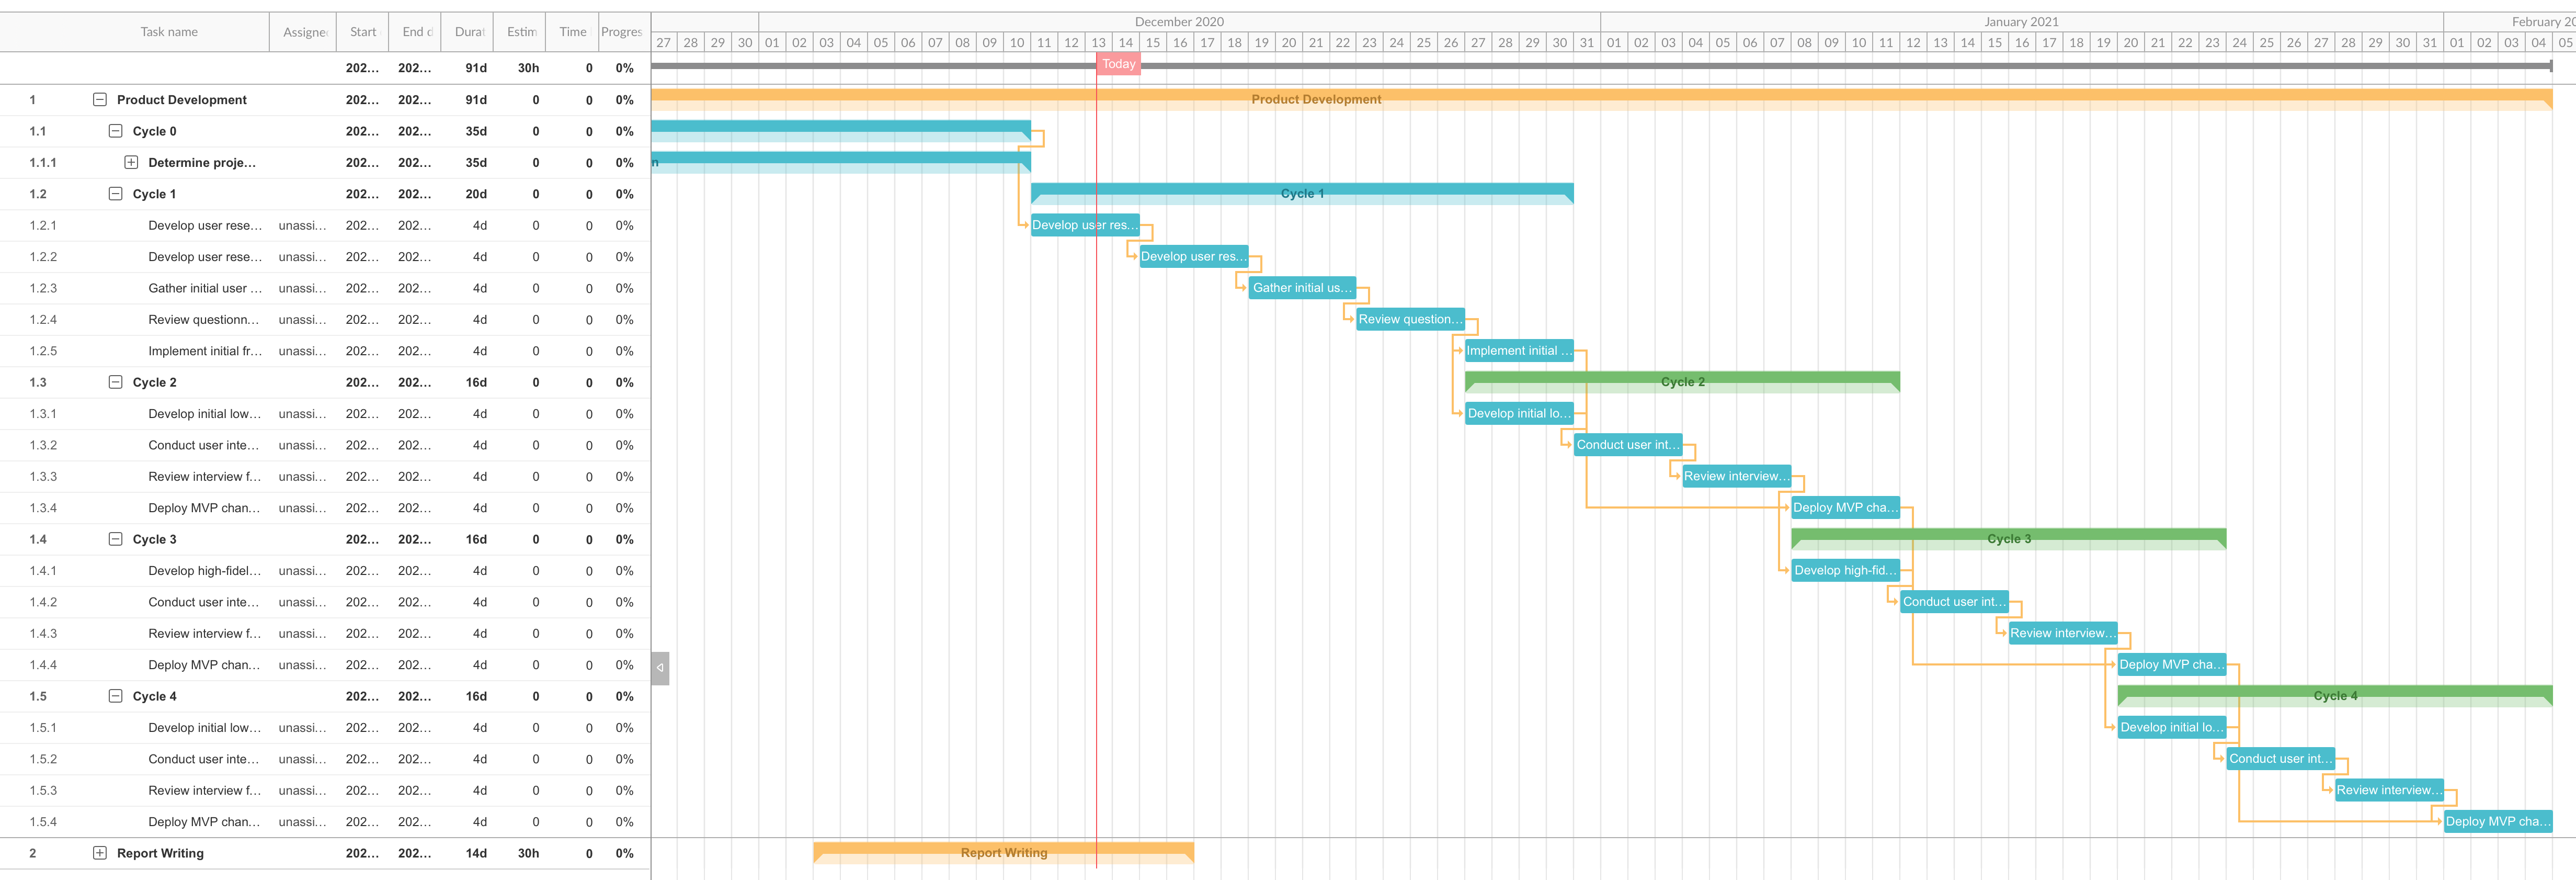
\includegraphics[width=\textwidth]{images/gantt.png}
    \caption{Illustration of the cycle-based project plan}
    \label{fig:gantt}
\end{figure}

\subsubsection{[BRAD] Milestones and Plan Updates} \label{sec:milestones_updates}
The main update to our working approach after starting the project was that we switched from two-week sprints to one-week sprints to ensure closer control and ensure delivery by the deadline, given the comparatively short project timeline. We decided to plan our sprints accordingly.

[BRAD] Can you create some kind of update to the Gantt chart?

\subsection{Team Roles}\label{sec:roles}

We used SCRUM as a methodology to assign basic team roles to work in an agile manner. The key roles involved a product owner, a scrum master, individual contributors and a QA lead.

In addition, all team members took on the role of representing personas for testing pursposes to ensure that we were not developing for ourselves, but rather for our users.

In terms of strict SCRUM roles, the team was allocated as follows (however, our responsibilities were treated fluidly as per the project's needs and in adherence to agile principles):

\begin{enumerate}
	\item \textbf{Aleksandar}: SCRUM master
	\item \textbf{Arjun}: Product owner
	\item \textbf{Blair}: Individual contributor
	\item \textbf{Brad}: QA lead
	\item \textbf{Hayato}: Individual contributor
\end{enumerate}

Within the team, our contributions were as follows:
\textbf{Aleksandar}  led definition of the technical architecture and software approach, and also led the implementation of user feedback specifically around the visual design.
\textbf{Brad}  led development of all tests, including the implementation of automated testing, and also contributed with developing parts of the application.
\textbf{Blair}  led much of the core applicationd development including the Slack authentication layer.
\textbf{Hayato}  worked on developing core parts of the application such as the grade leaderboards.
\textbf{Arjun}  supported with facilitating design workshops at the start, and later with some application development such as the grade calculation algorithm and documentation for the project.

\subsection{Market Benchmarking}
Initial desk research indicates that the selected project, a grades leaderboard, does not have a direct competitor. There are some utilities which partially solve the problem we are tackling - namely, tracking grades - but none of these enable the user to compare themselves to their peers, nor aggregates grade data. As such, we must cast a wide net to analyze our place in the market and consider \emph{alternative solutions}. We have identified utilities which overlap with our project in terms of possible user needs as well as tools which solve analogous problems in different domains in order to get a more comprehensive picture of where our product stands in the market.

Our solution offers two mains functions: \textbf{tracking grades} and \textbf{sharing/comparing} grades. For each feature, we have documented the alternative solutions, their specific functionality and notable design choices.

\subsubsection{Grade Tracking}
We surveyed various existing tools that enable students to track grades. Some peer-created utilities and University of London portal were discovered through our teammates' participation in this course, while \texttt{gpacalculator.io} \cite{gpa_calculator} is an example of many similar utilities that were found by searching 'grade tracking' and 'grade calculator' in a web search.

\paragraph{Peer student's Python command line grade calculator}
A peer student within the BSc Computer Science program at University of London developed a command line grades calculator \cite{lavoie_2020}. Users record their grades in a JSON file and run the script from the command line to see their grades and other relevant information, as shown in \cref{fig:py-calc}.

\begin{figure}[H]
\centering
\includegraphics[height=200pt]{brainstorm}
\caption{Python Calculator Sample Output}
\label{fig:py-calc}
\end{figure}

\subparagraph{Notable Features}
The tool allows tracking course-level and cumulative grades and converts to ECTS (Europe) and US scales. It also support conversion from US to UK GPA scores and determines which classification your grades fall into. Further, it allows tracking how many credits out of 360 were completed.

\subparagraph{Notable Design Choices}
The design is lightweight as it can be installed locally and run from a command line. The input is provided via a JSON file, which also allows easily storing, versioning and sharing a set of grades.

\paragraph{Peer's Google Sheets Degree Planner}
Another student (and co-author of this paper) has published a spreadsheet-based tool to track and calculate grades \cite{muralidharan_2020}. Users records their grades in a Google sheet to track their credits and grades, as shown in \cref{fig:deg-planner}.
\begin{figure}[H]
\noindent 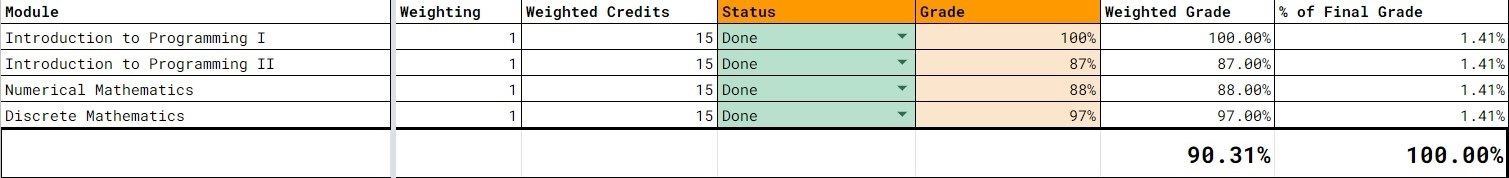
\includegraphics[width=\textwidth]{degree-planner-partial}
\centering
\caption{Google Sheets Degree Planner Excerpt}
\label{fig:deg-planner}
\end{figure}

\subparagraph{Notable Features}
The tool allows tracking course-level and cumulative grades, allows tracking how many credits out of 360 were completed and also highlights which modules are optional. It allows planning modules across semesters in order to distribute the course load.

\subparagraph{Notable Design Choices}
This tool is implemented with Google Sheets, which makes it easier to use for many people, and allows easy sharing of the tool as anyone has free access to the software without any local installation.

\paragraph{gpacalculator.io}

A publicly available website, GPA Calculator \cite{gpa_calculator}, allows users to enter their grades in a web form and see cumulative results, converted to various other grading standards.

\begin{figure}[H] 
\noindent 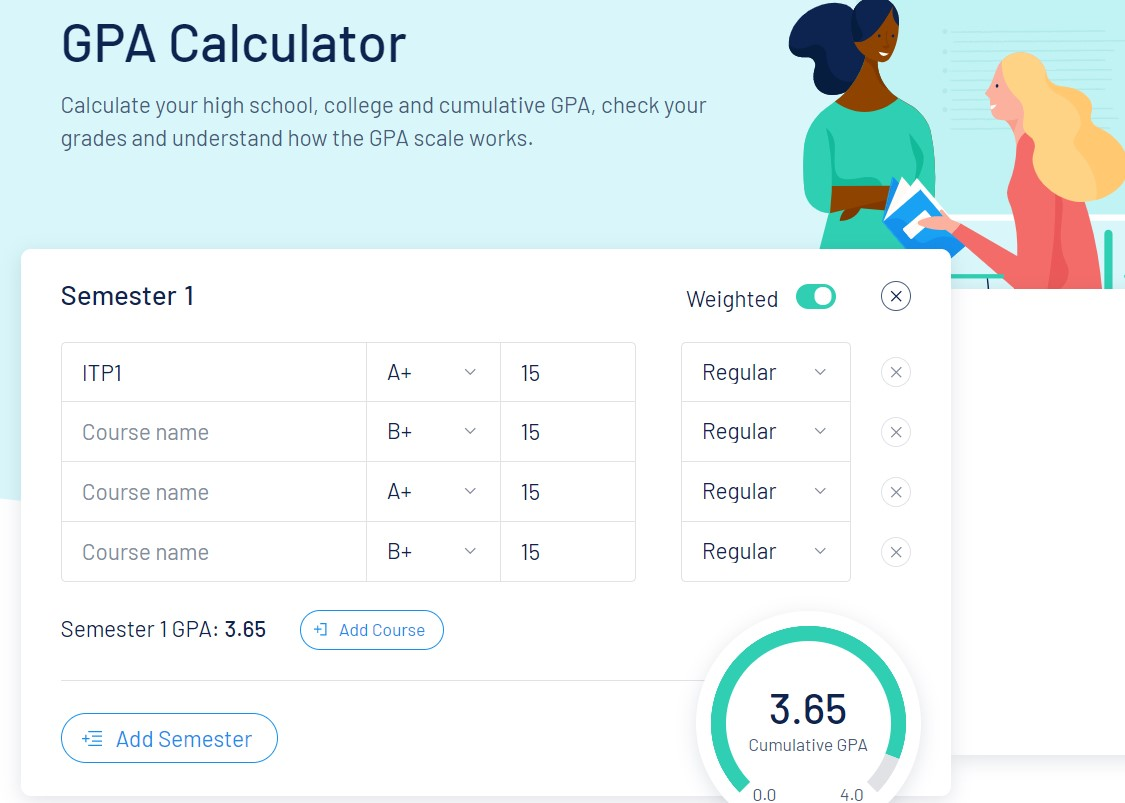
\includegraphics[width=8cm]{gpa-calculator-io}
\centering
\caption{Landing Page Form on gpacalculator.io}
\label{fig:gpa-calc}
\end{figure}
\medskip

\subparagraph{Notable Features}
The tool calculates semester or total cumulative GPA from individual courses, offers different calculators for high school and college and also provides general information about GPA, grades, and different honors.

\subparagraph{Notable Design Choices}
Placement of the input form is very prominent and users are immediately confronted with it when visiting the page. There is no login or data persistence available, and the tool is US-specific.

\paragraph{University of London Portal}

The University of London itself provides access to grades for viewing \cite{uol}. Users can view grades from each semester, broken down by source (coursework vs. exam), as shown in \cref{fig:uol-grades}

\begin{figure}[H]
\noindent 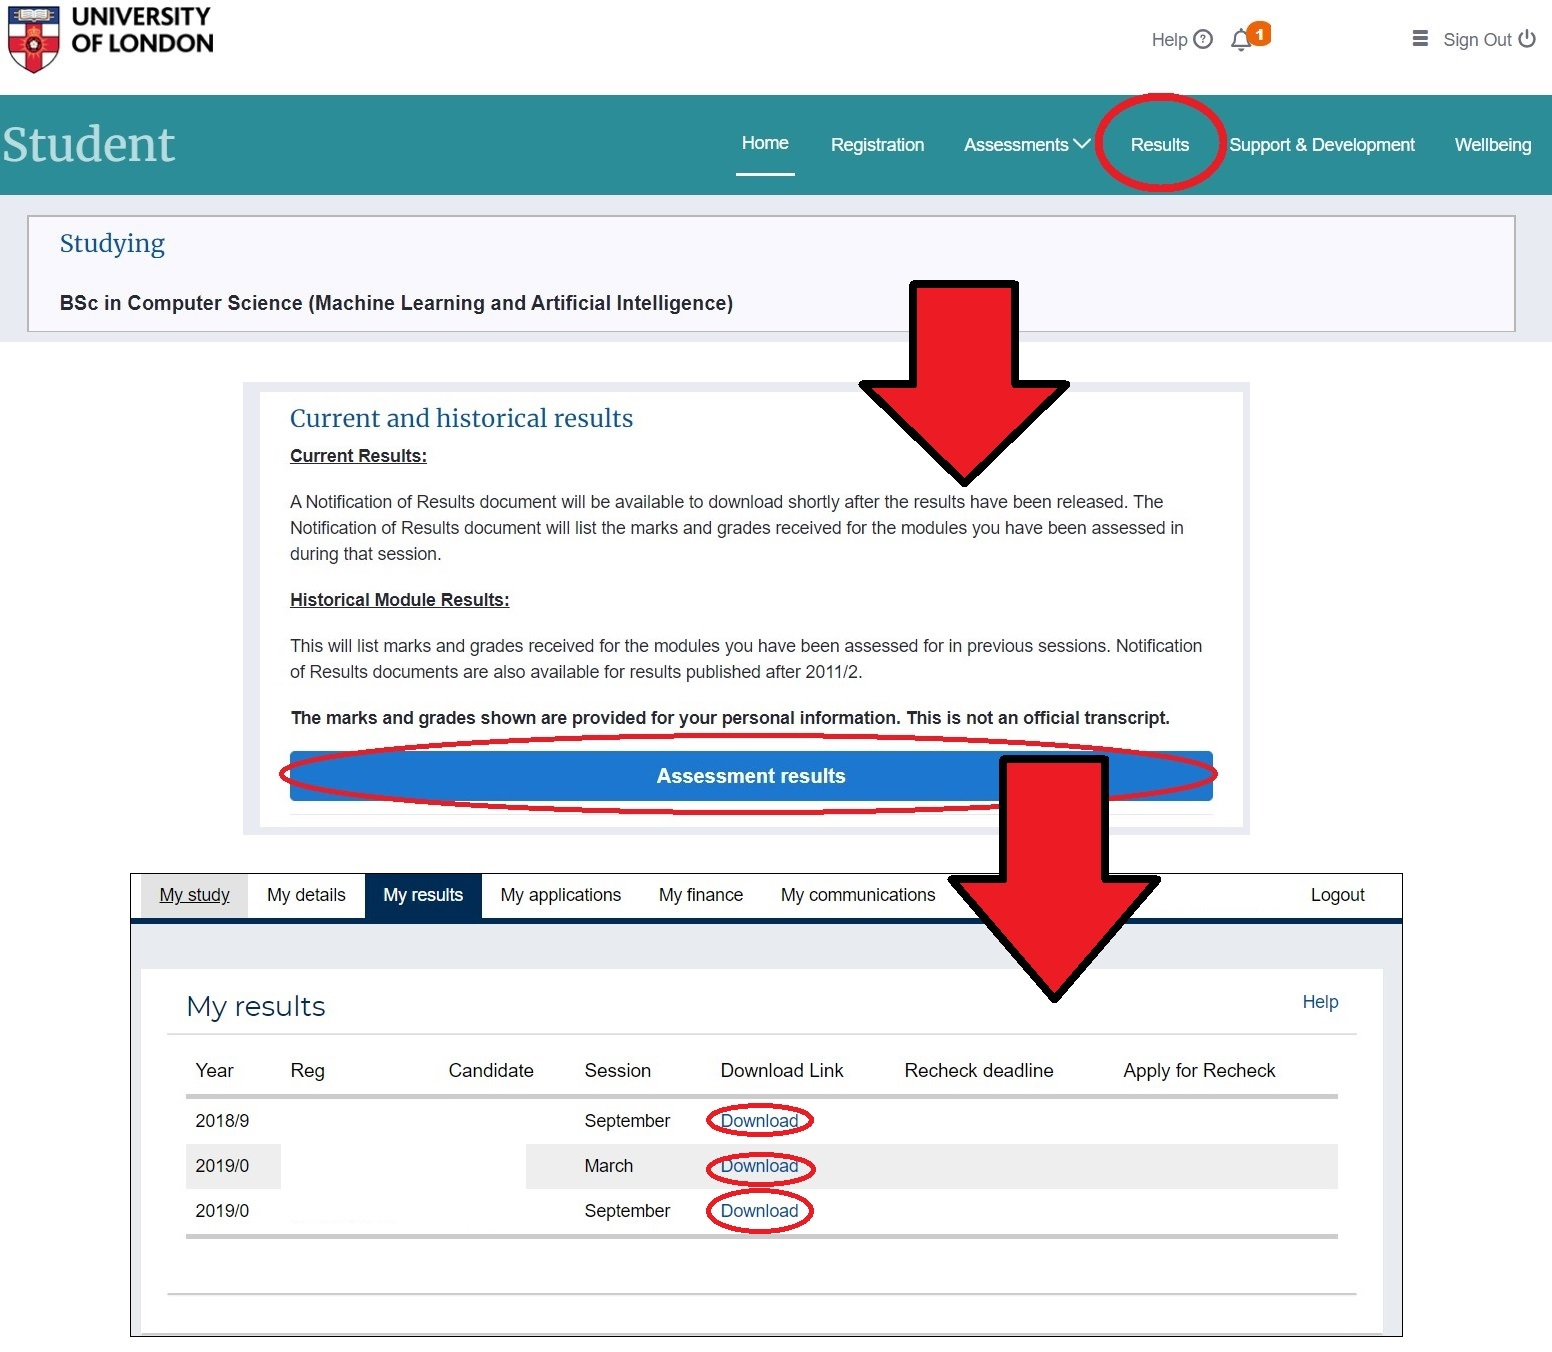
\includegraphics[height=250pt]{uol-buried}
\centering
\caption{Path to find grade download links on University portal}
\label{fig:uol-grades}
\end{figure}

\subparagraph{Notable Features}
The student portal displays official grade results for each semester and shows granular grades for each exam portion separately.

\subparagraph{Notable Design Choices}
Grades are not accessible easily, as they are buried in menus, and there is no centralized display of all grades or cumulative grades. A PDF download is required for all but the most recent grades. The results have the highest level of trustworthiness since they are official.

\subsubsection{Grade Sharing}

We searched the web for 'grade sharing,' 'grade comparing,' 'compare grades to other students,' and other derivatives but found no relevant tools. Glassdoor was suggested as an analogous tool during a brainstorming session and the University of London Slack workspace is known to us through our participation in the degree program.

\paragraph{University of London Slack workspace}

Students at the University of London's online BSc in Computer Science degree use a Slack workspace to collaborate \cite{slack}. Within this workspace, students enthusiastically share and query grade information following release of results, as shown in \cref{fig:slack-share}. This workspace is not publicly available.

\begin{figure}[H]
\noindent 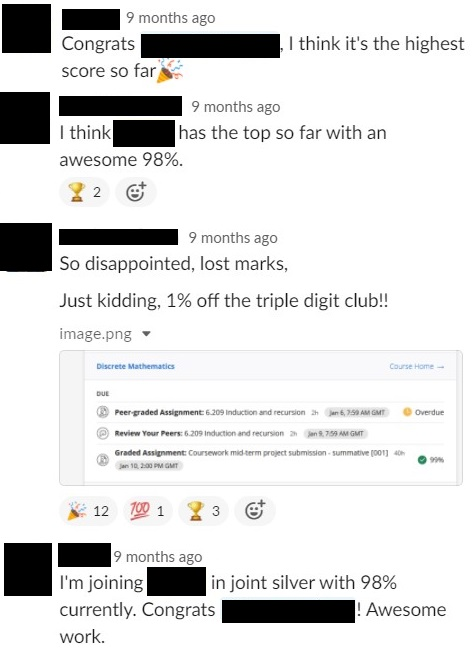
\includegraphics[height=200pt]{slack-share}
\centering
\caption{Students sharing midterm results on Slack}
\label{fig:slack-share}
\end{figure}

\noindent This is the Slack space open to all University of London online CS students. There are channels for each course. Grades are sometimes shared in threads after they are released.
\bigskip

\subparagraph{Notable Features}
Slack allows very quick impromptu sharing of grades, however on an irregular basis in bursts during grades season, and the grades are not solicited. Other students can weigh in and react or respond to grades and associated grade queries.

\subparagraph{Notable Design Choices}
Grades reported are usually biased towards students with high grades, or people with low grades who suspect an error in their results.

\paragraph{glassdoor.com}

Glassdoor is a review and reporting website for employers \cite{glassdoor}. It collects textual reviews and salary data from users. Salary reports are analogous to grade reports in that they are personal information about professional/academic performance that have a similar level of sensitivity.

\begin{figure}[H]
\noindent 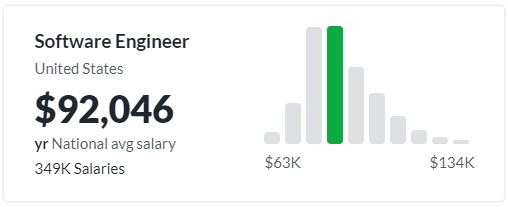
\includegraphics{glassdoor1}
\centering
\caption{Example of data and graph shown on glassdoor}
\label{fig:glassdoor-data}
\end{figure}

\subparagraph{Notable Features}
The site allows users to anonymously submit company reviews and salary information (including job title, locations of position, and years of experience). It contains job postings and company profiles with generic information. Users can also submit and collect job interview questions, and the site displays aggregate salary information for specific job titles.

\subparagraph{Notable Design Choices}

Users must submit a salary entry in order to view detailed salary information from other users. The salary collection form is not very prominent and not highlighted on the main site. Users can define their job title, often creating close duplicates of job titles.

\subsubsection{Summary of Market Benchmarks}
We abstracted a common set of functionality across these solutions as shown in \cref{tab:gradestrack} for grade tracking solutions, and \cref{tab:gradesshare} for grade sharing solutions.

\begin{table}[H]

\begin{tabular}{@{}rcccc@{}}
\toprule
                            & Python Grade Calc. & Degree Planner & gpacalculator.io & UoL \\ \midrule
Track Course Grades         &\checkmark               &\checkmark      &\checkmark        &\checkmark  \\
Calculate Cumulative Grades &\checkmark               &\checkmark      &\checkmark        &            \\
Track Credits               &\checkmark               &\checkmark      &\checkmark        &\checkmark  \\
Granular Grades             &                         &                &                  &\checkmark  \\
Convert Scales              &\checkmark               &                &                  &            \\
Determine Honors Level      &\checkmark               &                &                  &            \\
Persistence                 &\checkmark               &\checkmark      &                  &\checkmark  \\
Shareable                   &                         &\checkmark      &                  &            \\ \bottomrule
\end{tabular}
\caption{Grades Tracking Comparison}
\label{tab:gradestrack}
\end{table}


\begin{table}[H]
\centering

\begin{tabular}{@{}rcc@{}}
\toprule
                                & UoL Slack & glassdoor.com \\ \midrule
Incentivized to submit data     &           &\checkmark     \\
Can compare to others           &\checkmark &               \\
Easy to reference               &           &\checkmark     \\
Aggregates data                 &           &\checkmark     \\
Includes profile on data source &           &\checkmark     \\
\bottomrule
\end{tabular}
\caption{Grades Sharing Comparison}
\label{tab:gradesshare}
\end{table}

\subsection{Market Positioning}
In order to understand our solution's place in the market we need to examine the external factors which might affect the growth and performance of our application.

In the following section we perform both a STEEPLE \cite{bowman_1998} analysis as well as a SWOT \cite{panagiotou_2003} analysis to support identifying the correct market position.

\subsubsection{STEEPLE Analysis}
The STEEPLE analysis will allow us to analyse our problem space based on environmental factors and outlines some of the contextual consequences of our proposal.
\medskip

\noindent \textbf{Social}
\begin{itemize}
    \item People tend to be competitive \cite{hutson_2015}
    \item People may be hesitant to share if their grades are low or they feel they are unfairly graded
\end{itemize}
\textbf{Technological}
\begin{itemize}
    \item Student's participation in the course ensures they will have the hardware necessary to access the website (computer or mobile and internet)
\end{itemize}
\textbf{Economic}
\begin{itemize}
    \item Global audience means any potential efforts to monetize users would be subject to currency risk and local purchasing power
    \item Usage costs and any potential revenue would be related to enrollment in University of London program and size of other Universities
\end{itemize}
\textbf{Environmental}
\begin{itemize}
    \item Server has energy requirements that will grow with usage
    \begin{itemize}
        \item An increasing number of cloud providers offer solutions that use green energy
\end{itemize}
\end{itemize}
\textbf{Political}
\begin{itemize}
    \item Regulation of data handing is increasing everywhere. This continued trend is exemplified by recent regulations enacted over the past two years:
    \begin{itemize}
        \item Califonia, USA's CCPA
        \item EU's GDPR
        \item Canada's PIPEDA
        \item Japan's APPI 
        \item Brazil LGPD
    \end{itemize}
    Given the global nature of this degree program our application is sensitive to all of these policies and future data protection measures implemented worldwide
\end{itemize}
\textbf{Legal}
\begin{itemize}
    \item Must comply with local data protection regulations listed above
\end{itemize}
\textbf{Ethical}
\begin{itemize}
    \item Must handle sensitive data responsibly and transparently
    \item Obligated to maintain a healthy sense of competition and steer away from toxicity and envy
    \item Honest reporting of grades and integrity of reported data is critical
\end{itemize}
\bigskip

\noindent \subsubsection{SWOT Analysis}
The SWOT analysis supports the identification of our solution's underlying potential and associated risks.
\smallskip

\noindent \textbf{Strengths}
\begin{itemize}
    \item Knowing you have a relatively high grade could be motivating / encouraging / validating.
    \item Validation if your grade was low but many people report similar grades.
    \item Highlights which courses may be more difficult and require additional focus.
    \item Helps students understand when their grades may be unjustifiably low, which may help in organizing a more detailed and thoughtful request to the institution to review the grades or rubric.
    \item Comparison aspect provides motivation for maintaining one's standing at or above a certain percentile.
    \item The leaderboard aspect "gamifies" grades and gives incentive to submit grades.
    \item Ability to see module "reviews" and retrospectives might be an additional motivator for students
\end{itemize}
\textbf{Weaknesses}
\begin{itemize}
    \item Data reliability. We have no good way to validate data so we must dis-incentivize dishonesty and not assume 100\% accuracy. This might be solved with a voluntary "random check" participation where students need to prove that they actually received these grades
    \item A small sample size of participants will limit usefulness of averages.
    \item Those with poor marks or marks they feel are unjustified will likely be less willing to share.
    \item Those who fail or drop out may be unable (depending on integration) or unwilling to participate, which could impact grade averages.
    \item Without a representative sample of students the averaged data, graphs, etc will be skewed and could lead to reduced acceptance or usage of the tool.
    \item If we report anonymously, do we also store anonymously? If so then do we provide for the ability to remove data on request?
\end{itemize}
\textbf{Opportunities}
\begin{itemize}
    \item This project has few real competitors. There are some student created utilities but grade sharing/comparing is outside the scope of those utilities.
    \item The program size will continue to grow for a long time. We haven't reached the maximum number of cohorts and the recent cohorts have grown. The need exists, there just wasn't a reason to make it until now.
    \item If we are the first to make this, we can capture the interested user-base which should be a large moat.
    \item Slack integration allows us to naturally link to the community of students that already exists, leveraging the University's policing of that population to being actual students.
    \item Retrospective tips can be used by future cohorts to gain a studying advantage for the course
    \item Average grades per course, per semester, etc can similarly help future students know what to expect and perhaps how much they need to prepare
\end{itemize}
\textbf{Threats}
\begin{itemize}
    \item Time. Other student utilities show recognition of value for this type of product. Probably only a matter of time until someone else extends the grade idea in a similar fashion.
    \item Leak or theft of personally identifiable grade and contact information.
    \item People could poison the data with dishonest grade reporting.
    \item Insecure design could compromise data integrity and give people access to sensitive information.
    \item Loss of integration / changes to any APIs we're using (such as Slack).
    \item Data loss.
\end{itemize}



\subsection{Customer Survey}
As of this report, the team has designed the high-level questions that should be answered by data recording. Our key research questions are listed below. Note that these are not the actual survey questions, but rather the questions we aim to answer through our data recording and analysis.

\begin{itemize}
    \item How do students currently keep track of grades?
    \item How comfortable are students with sharing their grades?
    \item How honest will people be with reporting their grades, anonymously or not?
    \item Why would students want to compare their grades with other students?
    \item Why would students want to see retrospective tips left by other students?
    \item Why is this different from just getting the (presumably anonymized) values from the University? Why is this better?
    \item Would there be value in providing automated conversion of grades from the UK standard to standards from other countries?
    \item Does anonymity encourage or hinder contribution to the leaderboards? Does it affect accuracy of reporting?
\end{itemize}

Data gathering will be conducted via an online survey among university students, and interviews will be conducted via online video calls with selected university students.

\subsubsection{Online Survey - Design Choices}

We used the online survey to gather quantitative data. Not all of our key research questions can easily be answered quantitatively so we will seek to answer these in the student interviews.

We created the survey by converting key research question to a survey question designed to elicit the required answers where able. We did not require any questions to submit the survey because we felt it was important to ensure reliable answers and wanted to ensure the highest possible response rate. The survey was only 8 questions and took approximately 2 minutes to fill out in order to encourage a higher response rate. We provided context of our project before asking the following questions.

We posted the survey in this course's \textit{general} slack channel. The survey respondents are the potential users so the responses can be considered representative of our real users.

\subsubsection{Online Survey - Questions and Results}
Following are the questions we asked to start collecting data on our key research questions, followed by the results.

\textbf{1. Key Research Question:} How do students currently keep track of grades?
\smallskip

\textbf{1a. Survey Question:} What tools do you use to keep track of grades?
\smallskip

\textbf{Results:}

\begin{table}[H]
\centering
\begin{tabular}{@{}lc@{}}
\toprule
                  & {\textbf{Responses}}  \\ \midrule
\textbf{University of London Portal}    & 68.4\%    \\
\textbf{Outside Tool}                   & 47.3\%    \\
\textbf{None}                           & 15.8      \\ \bottomrule
\end{tabular}
\caption{What tools do you use to keep track of grades?}
\label{survey1a}
\end{table}

\textbf{2. Key Research Question:} How comfortable are students with sharing their grades?
\smallskip

\textbf{2a. Survey Question:} Have you ever shared your overall course or individual assessment grades in slack?
\smallskip

\begin{table}[H]
\centering
\begin{tabular}{@{}lc@{}}
\toprule
                  & {\textbf{Responses}}  \\ \midrule
\textbf{Yes}    & 52.6\%    \\
\textbf{No}     & 47.4\%    \\ \bottomrule
\end{tabular}
\caption{Have you ever shared your overall course or individual assessment grades in slack?}
\label{survey2a}
\end{table}

This question helps us establish a behavioral baseline for student comfort in sharing grades. We ask about past behavior to get the most objective answers possible. We also surveyed students for their sentiment on this key research question.
\medskip

\textbf{2b. Survey Question:} How comfortable are you with sharing grades with other students?
\smallskip

\begin{table}[H]
\centering
\begin{tabular}{@{}lc@{}}
\toprule
                  & {\textbf{Responses}}  \\ \midrule
\textbf{At least somewhat comfortable}    & 79.9\%    \\
\textbf{Not comfortable}     & 21.1\%    \\ \bottomrule
\end{tabular}
\caption{How comfortable are you with sharing grades with other students?}
\label{survey2b}
\end{table}

\textbf{2c. Survey Question:} What would make you more comfortable sharing grades?
\smallskip

\textbf{Results:}

\begin{table}[H]
\centering
\begin{tabular}{@{}lc@{}}
\toprule
                  & {\textbf{Responses}}  \\ \midrule
\textbf{Anonymity}    & 73.7\%    \\
\textbf{Evidence of Privacy Protections}     & 52.6\% \\
\textbf{Seeing other students using tool}     & 47.4\% \\
\textbf{Knowing grades can only be viewed by students}     & 36.8\% \\
\textbf{Open source with transparent developers}     & 31.6\% \\
\textbf{University endorsement}     & 21.1\%\\ \bottomrule
\end{tabular}
\caption{What would make you more comfortable sharing grades?}
\label{survey2c}
\end{table}

\textbf{3. Key Research Question:} How honest will people be with reporting their grades, anonymously or not?
\smallskip

\textbf{3a. Survey Question:} How would you feel about submitting a low grade anonymously?
\smallskip

\begin{table}[H]
\centering
\begin{tabular}{@{}lc@{}}
\toprule
                  & {\textbf{Responses}}  \\ \midrule
\textbf{Indifferent}    & 73.7\%    \\
\textbf{Good}     & 26.3\%    \\ \bottomrule
\end{tabular}
\caption{How would you feel about submitting a low grade anonymously?}
\label{survey3a}
\end{table}

\textbf{3b. Survey Question:} How would you feel about submitting a low grade publicly?
\smallskip

\begin{table}[H]
\centering
\begin{tabular}{@{}lc@{}}
\toprule
                  & {\textbf{Responses}}  \\ \midrule
\textbf{Indifferent}    & 78.9\%    \\
\textbf{Bad}     & 21.1\%    \\ \bottomrule
\end{tabular}
\caption{How would you feel about submitting a low grade publicly?}
\label{survey3b}
\end{table}

\textbf{4. Key Research Question:} Why would students want to compare their grades with other students?
\smallskip

\textbf{4a. Survey Question:} Please rate to what degree each of the following are important reasons for contributing grades. 1 is not important, 5 is very important.

\textbf{Results:} To determine the most important reasons, we consider a 4 or 5 an "endorsement." The endorsements ranked from high to low:

\begin{table}[H]
\centering
\begin{tabular}{@{}lc@{}}
\toprule
                  & {\textbf{Endorsements}}  \\ \midrule
\textbf{See Where I Rank Against Other Students}    & 13    \\
\textbf{Track Grades}     & 10 \\
\textbf{Keep University Grading Curve Transparent}     & 9 \\
\textbf{Help Upcoming Cohorts}     & 6 \\
\textbf{Recognize High Achievers}     & 5 \\ \bottomrule
\end{tabular}
\caption{Most important reasons for contributing grades}
\label{survey4a}
\end{table}

\textbf{5. Key Research Question:} Why would students want to see retrospective tips left by other students?
\smallskip

\textbf{5a. Survey Question:} Please rate to what degree each of the following are important reasons for leaving retrospective tips for courses. 1 is not important, 5 is very important.

\textbf{Results:} Like the previous question, we considered a 4 or 5 an "endorsement." The endorsements ranked from high to low:

\begin{table}[H]
\centering
\begin{tabular}{@{}lc@{}}
\toprule
                  & {\textbf{Endorsements}}  \\ \midrule
\textbf{Learn from wisdom of others}    & 15    \\
\textbf{Assessing course expectations}     & 15 \\
\textbf{Assessing effort course}     & 13 \\
\textbf{Give back to community}     & 12 \\
\textbf{Choosing courses to take}     & 12 \\ \bottomrule
\end{tabular}
\caption{Most important reasons for leaving retrospective tips for courses}
\label{survey5a}
\end{table}

\subsubsection{Online Survey Insights}
\cref{survey2a} shows a majority of respondents (52.6\%) have shared their grades in slack. Slack is not anonymous and there is no explicit place to share so these students who shared can be considered highly motivated to do so. In addition, a large majority (79.9\%) report feeling comfortable sharing their grades in an unqualified manner (neither anonymous or public specified), as shown in \cref{survey2b}. In addition, \cref{survey1a} shows nearly 50\% of respondents already use an external tool to calculate their grades. These responses strongly confirm that there is demand for a tool that allows people to share and compare grades.

Responses also reveal that anonymity is key. We see in \cref{survey2c} that a large majority (73.7\%) of respondents said anonymity would make them more comfortable sharing grades. This was the single largest factor for making students more comfortable in sharing grades. In addition, 73.7\% of respondents said they felt indifferent about sharing low grades anonymously and 0\% reported feeling bad about it in \cref{survey3a}. Whereas 78.9\% reported that they would feel bad about sharing a low grade publicly and only 21.1\% said they would feel indifferent in \cref{survey3b}. Therefor anonymity is crucial for increasing participation and integrity of grades.

\section{Prototyping and Iteration}
\subsection{Techniques}
Our strategy towards prototyping will focus on creating a number of low-fidelity prototypes to quickly iterate on, while high-fidelity prototypes will consist of actual software that we can test. We will not create detailed up-front designs or clickable prototypes for the reason that our application's core functionality can easily be communicated with low-fidelity prototypes.

The reasoning for this approach lies in the economic principle of prototyping, which states that the best prototype is one that can demonstrate the possibilities and limitations of a solution in the most efficient manner.

\subsection{Storyboards \& Sketching}
The team developed initial storyboards to illustrate the user journey and make the value proposition tangible. A series of sketches is embedded for the identified personas in \cref{fig:storyboard_competitive} and \cref{fig:storyboard_casual}. Based on these storyboards, we learned the following:
\begin{itemize}
    \item The main motivation to log on is likely the need to track grades in a central, easily accessible location that also calculates averages automatically
    \item There are peak times during the year that the tool will see higher usage (e.g. when grades are released)
    \item Students are interested in the distribution of grades on a curve
\end{itemize}

The team will consider these factors in the development of the solution.

\begin{figure}[H]
    \centering
    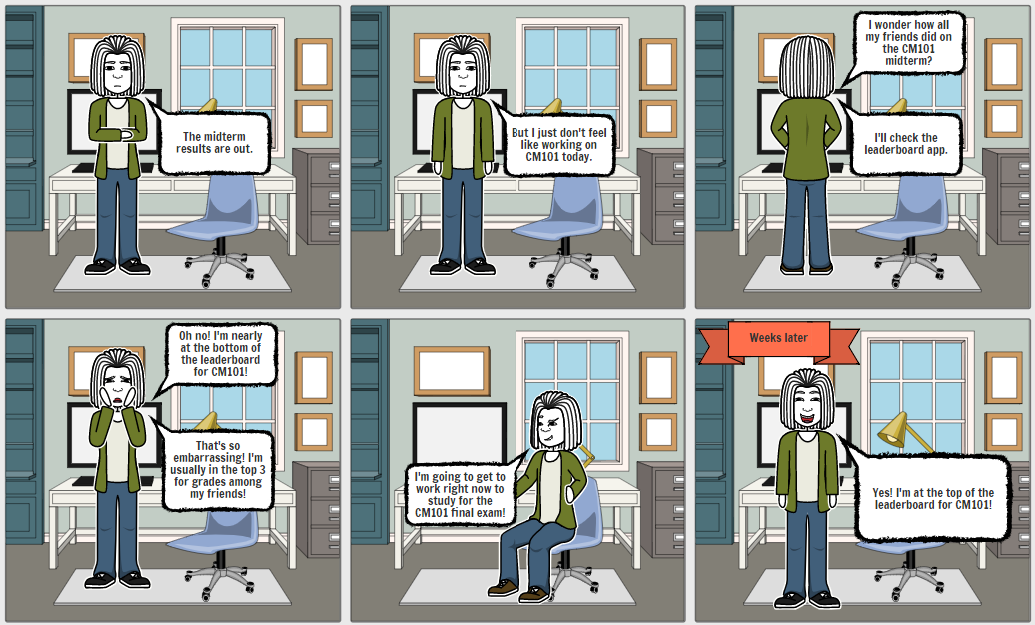
\includegraphics[width=0.95\textwidth]{competitive_topper_1.png}
    \caption{Initial storyboard for the persona ``Competitive Topper''}
    \label{fig:storyboard_competitive}
\end{figure}

\begin{figure}[H]
    \centering
    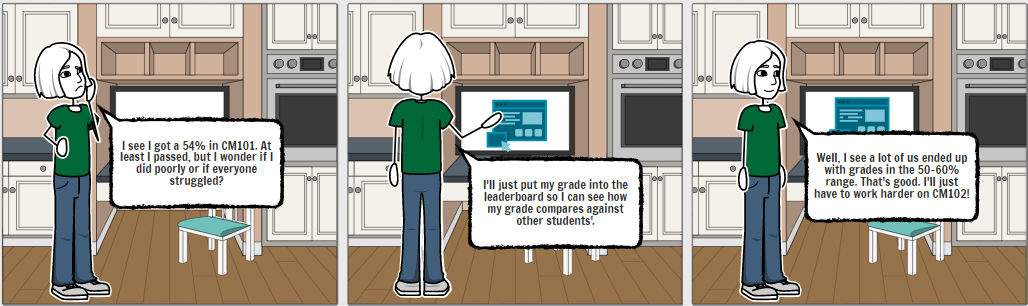
\includegraphics[width=0.95\textwidth]{casual_checker_1.png}
    \caption{Initial storyboard for the persona ``Casual Checker''}
    \label{fig:storyboard_casual}
\end{figure}

\subsection{Wireframes}
To further illustrate how the application will work, an initial wireframe was created to show how an entry page to capture grades might look like. This wireframe was built using a wireframing tool (Balsamiq)\cite{balsamiq} and will be iterated on as we move towards building the solution.

\begin{figure}[H]
    \centering
    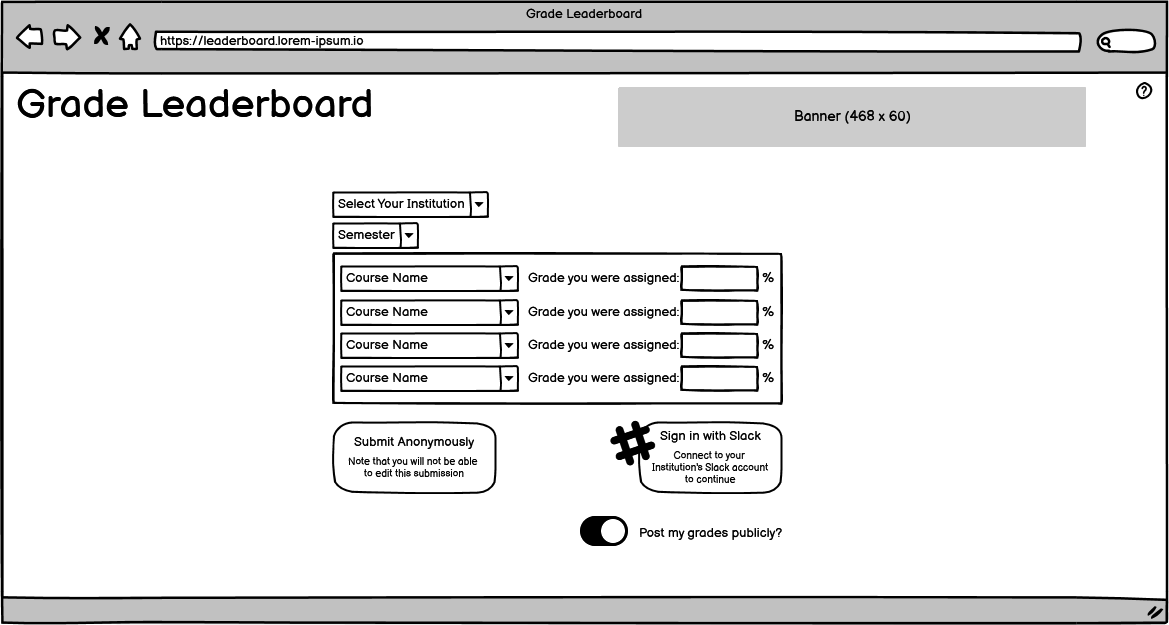
\includegraphics[width=\textwidth]{images/Initial Page.png}
    \caption{Early wireframe sketch}
    \label{fig:earlywireframe}
\end{figure}

Based on this very early wireframe, the team identified important questions to consider for further iteration.

\begin{itemize}
    \item Should users enter to see their own overview of grades, or an aggregate?
    \item How might users authenticate into the system?
    \item How does an aggregated view look?
    \item What other information might we need to collect from users?
\end{itemize}

As a result of these questions and collaboration further iterations were made to the early wireframe. As well, initial versions of a login page, a report view, and a grade leaderboard were developed by the group.

\begin{figure}[H]
    \centering
    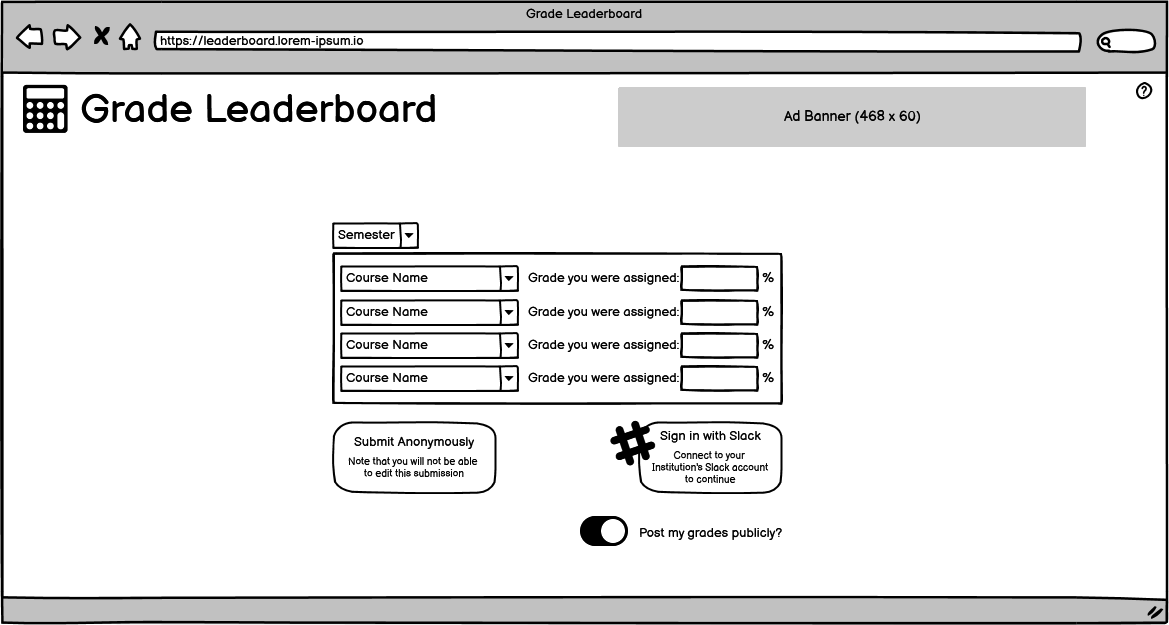
\includegraphics[width=\textwidth]{images/Initial Page v07.png}
    \caption{Wireframe after group iteration}
    \label{fig:modifiedwireframe}
\end{figure}
\begin{figure}[H]
    \centering
    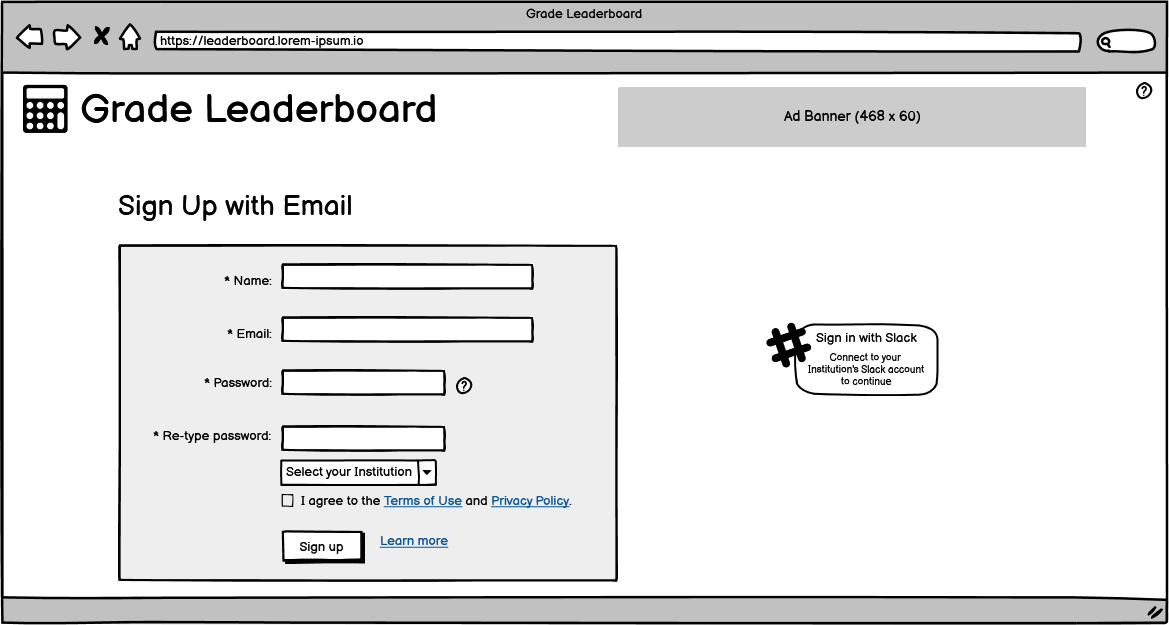
\includegraphics[width=\textwidth]{images/Sign in Page v07.png}
    \caption{Initial signin page wireframe}
    \label{fig:signinwireframe}
\end{figure}
\begin{figure}[H]
    \centering
    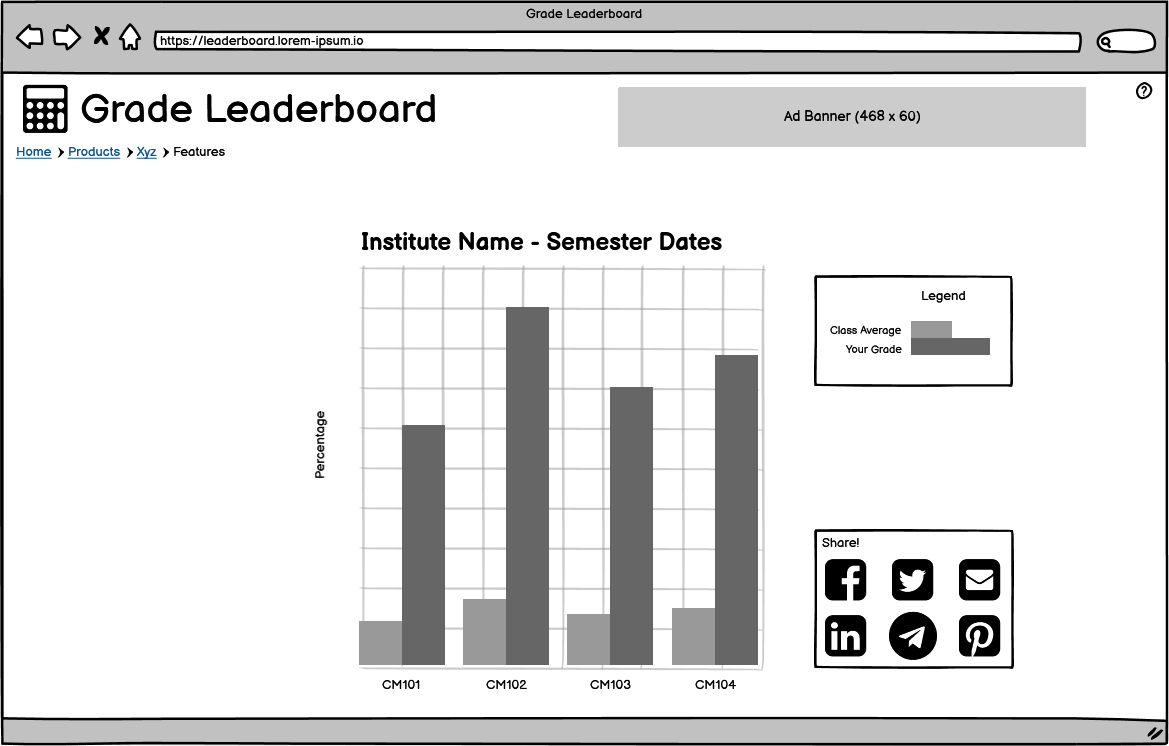
\includegraphics[width=\textwidth]{images/Full semester - class averages chart 1 v07.png}
    \caption{Early collaboration on report wireframe}
    \label{fig:earlyreportwireframe}
\end{figure}
\begin{figure}[H]
    \centering
    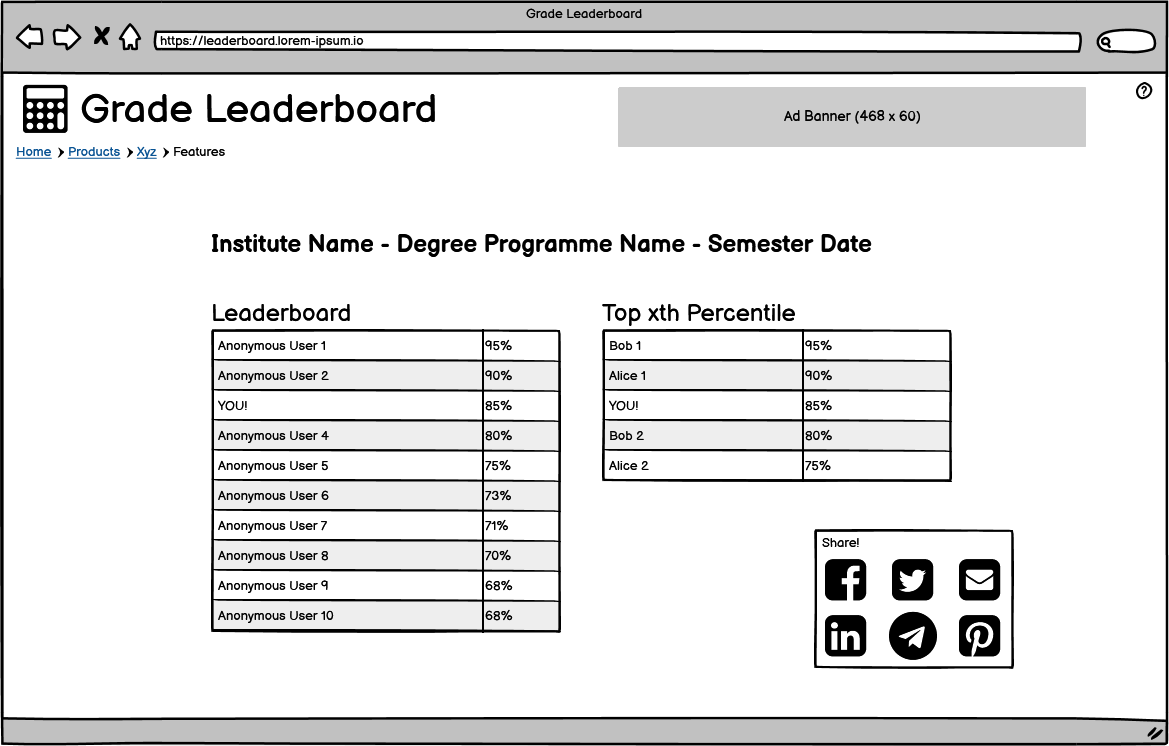
\includegraphics[width=\textwidth]{images/One course - Leaderboard v07.png}
    \caption{Early leaderboard wireframe}
    \label{fig:earlyleaderboardwireframe}
\end{figure}

\section{Design}
\subsection{Iterative Design}\label{sec:iterative_design}
Requirements gathering for this project are based on a classical ``double diamond'' approach. In order to create this proposal, the project team has iterated once internally to gather a potential set of very high-level critical functionality to inform further data gathering. We explored potential topics of interest, narrowed it down to the topic of creating a grade comparison tool for university students, and then explored the problem space.

\begin{figure}[H]
    \centering
    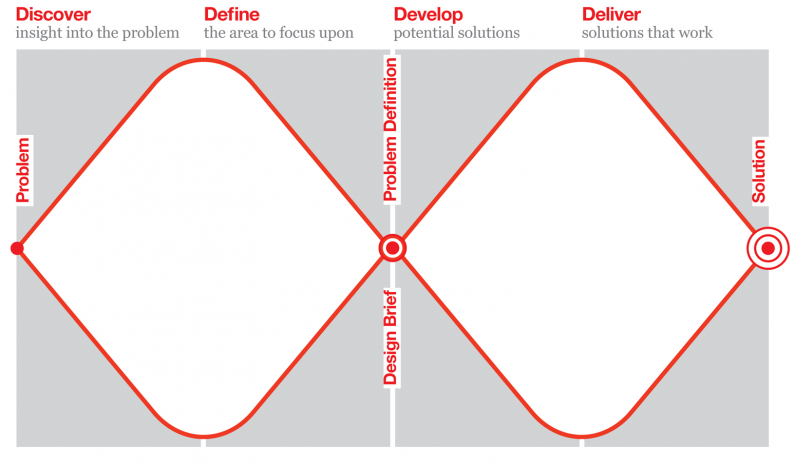
\includegraphics[width=10cm]{images/Double-Diamond-A3-for-publication-A-2000px_1.png}
    \caption{Double Diamond Design Approach}
    \label{fig:doublediamond}
\end{figure}

The reason why we chose the double diamond method is because it is widely used in Design Thinking \cite{interaction_design} approaches when project ambiguity is high. The team felt this approach would lead to the highest level of clarity quickly, and would fit into the given timelines by the course schedule and the available capacities of the team.

We considered alternatives such as the Google Design Sprint, but eventually decided not to pursue this as we were not in the need of a 5-day, rapid iteration approach for our solution. We might use it partially during more concrete stages of the project to accelerate progress. We also considered "Research in the wild" (RITW) to find disruptive behaviour-changing ideas, however this approach felt inappropriate as our problem space did not indicate a fundamental challenge to existing technology, but much rather the fulfilment of a basic need of university students often not provided by universities.

\subsection{Discovery}
As background for how we arrived at our final idea, we initially conducted a number of broader exercises to discover potential problem spaces. The team conducted a ``Crazy 8'' exercise in which each team member developed at least 8 new ideas in a time span of a minute for each idea. This laid out a large space of potential ideas the team could work on.

\begin{figure}[H]
    \centering
    \includegraphics[width=\textwidth]{images/brainstorm.png}
    \caption{Illustration of initial discovery exercise}
    \label{fig:brainstorm}
\end{figure}

Next, we used dot-based voting to narrow down the ideas to those with the highest assumed potential for success and highest interest for the group to further explore. 

Once we had narrowed the ideas down from over 40 to just 5, we decided to explore the potential problem space for each via mind maps, exploring the potential competitive landscape, possible functionality and target users.

\begin{figure}[H]
    \centering
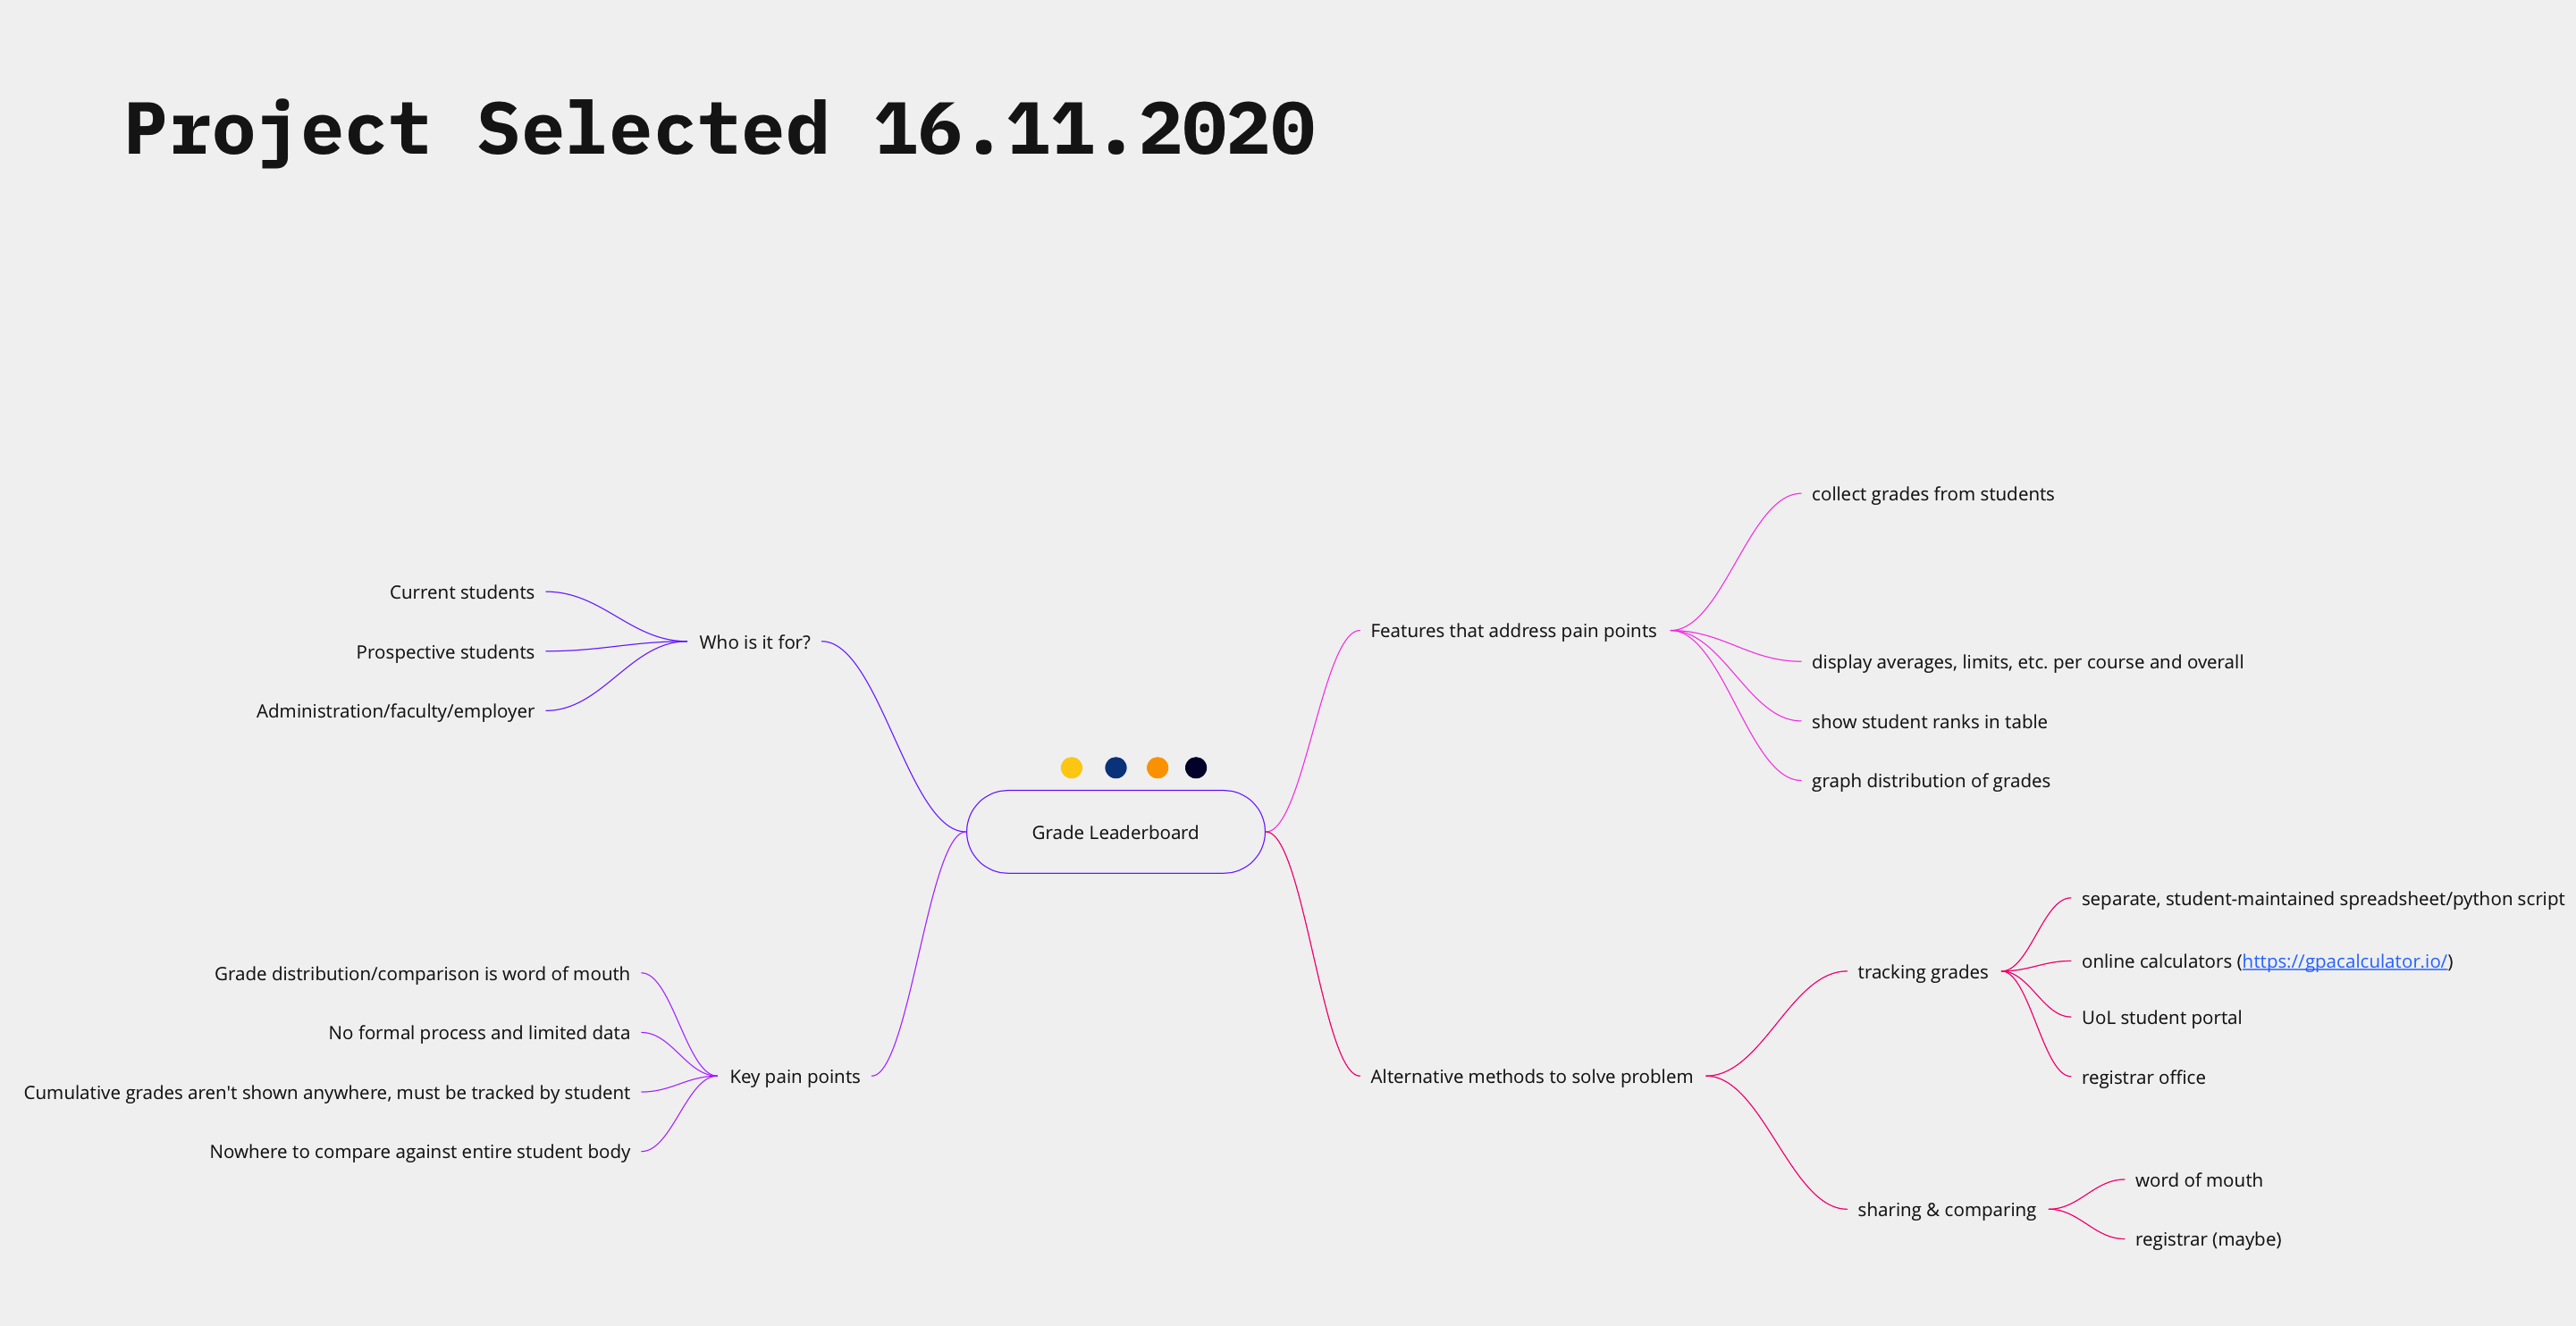
\includegraphics[width=\textwidth]{images/mindmap.png}
    \caption{Mindmap for the winning idea}
    \label{fig:mindmap}
\end{figure}

To further explore the problem space of student grading, we began by brainstorming potential functionality. 

\subsection{High-Level Requirements Funnel}

Our approach to gathering requirements will follow these phases, based on the approach for data gathering and requirements analysis described in \cite{sharp_2019}.

\begin{enumerate}
    \item \textbf{Data Gathering}: We first use two methods for data recording, namely \textit{questionnaires} and \textit{interviews}. These will serve as initial data input for the project. This will be aided by further desk research to inform the problem space, such as academic papers in the area.
    \item \textbf{Data Analysis}: Analysis of data recorded in this manner will occur based on the analytic framework of \textit{content analysis} and \textit{grounded theory}. We will both develop quantitative and qualitative analysis based on the recorded data. We aim to formulate our \textbf{core hypotheses} around this analysis. At the point of writing this paper, only quantitative data had been gathered, with more input following in early 2021.
    \item \textbf{Formulate requirements}: Finally, we develop requirements in the form of epics and user stories. To aid this process, we decided to use the frameworks of \textit{contextual inquiry}, which allows us to discover requirements that inspire \textit{joy of use} and \textit{joy of life}, and the 7 product dimensions \cite{gottesdiener_gorman_2014}, which allow us to ensure broad coverage of important product attributes.
\end{enumerate}



\subsection{Initial Epics}
Based on the survey results and research to date, we have identified initial epics, formulated in story format with acceptance criteria. The acceptance criteria would be further broken down into user stories that fulfill those criteria.

\paragraph{Capture Grades} As a student, I want to enter a  module  grade,   so  that  I can  contribute  to  the  data-base and help other students.
\subparagraph{Acceptance Criteria}
\begin{itemize}
    \item Only authenticated users can provide a grade
    \item Grades can be submitted anonymously
    \item Capturing a grade is fast and requires little input
    \item One student can only capture one grade per module
    \item Students can update a previously captured grade
\end{itemize}

\paragraph{View Grades} As a student, I want to view all the grades for a specific module, so that I can see how I compare with other students.
\subparagraph{Acceptance Criteria}
\begin{itemize}
    \item Students can see their position on a leaderboard for the entire program
    \item Students can see their position on a leaderboard for a single module
    \item Students can see the distribution of grades for the entire program
    \item Students can see the distribution of grades for a single module
\end{itemize}


\paragraph{Manage Personal Grades} As a student, I want to to capture and manage all my grades in my program, so that I can see my program progress and calculate my final grade.
\subparagraph{Acceptance Criteria}
\begin{itemize}
    \item Students can view all their program grades in a single overview
    \item Students can assign modules to semesters that they plan to take
    \item Grades are used to calculate a program average using the correct weighting and credits
    \item Students can see their program progress as a percentage
\end{itemize}

\paragraph{Submit Module Retrospectives} As a student, I want to to submit a module retrospective, so that I can inform other students about my experience.
\subparagraph{Acceptance Criteria}
\begin{itemize}
    \item Students can enter a free-text retrospective assigned to a specific module
    \item Students can only enter one retrospective per module
    \item Students can assign ratings to effort and difficulty of a specific module
    \item Students can see retrospectives entered by them
\end{itemize}

\paragraph{View Module Retrospectives} As a student, I want to to read module retrospectives submitted by other students, so that I can make an informed choice about future modules.
\subparagraph{Acceptance Criteria}
\begin{itemize}
    \item Students can see a list of modules and sort it by rating criteria
    \item Students can read retrospectives entered for a specific module
\end{itemize}

As part of development, we will prioritize these epics and likely deliver on a subset of them in the initial release.

\subsection{[ARJUN] Justification of Design Decisions}\label{sec:justif}


\section{Testing}\label{sec:testing}

\subsection{General methodology}
The team decided that the most appropriate evaluation type is in a \textbf{controlled settings directly involving users}. This means having users peruse the product under observation, describing their experience and providing live feedback. This will be the most efficient approach from a planning perspective.

A further reason this is more appropriate as opposed to \textit{natural settings} is that grades are not something students submit and engage with on a daily basis, hence the opportunities to observe students in this process are rare. This will result in certain downsides of the controlled setting taking precedence, specifically not being able to identify behaviours of users that may occur when unsupervised, which may be central to the grades process. A future iteration may employ screen recording (such as Hotjar) or A/B testing to identify more hidden behaviours. An UMUX-Lite method for evaluating usability will be employed based on \cite{lewis}.

We will test the produced application at the end of each cycle with 1-3 real student users, recording the outcomes and discussing the results along four categories:

\begin{enumerate}
    \item \textbf{Likes}: What did users enjoy about the product?
    \item \textbf{Problems}: What problems did users encounter while using the product?
    \item \textbf{Ideas}: What are new impulses that users provided while using the product?
     \item \textbf{Questions}: What questions did users ask while using the product?
\end{enumerate}

\subsection{Formative Testing}\label{sec:formative}
\subsubsection{Identifying Users}
In order to identify users, we employ the technique of personas to help identify the right kind of user. We also employ \textit{scenarios} and user fiction to describe the kind of experience we envision for end users.

The underlying hypothesis for our personas is that some users will be more interested in such a tool than others, and do so for different purposes. Our hypothesis is based on the observation that among our own cohort of students in the program, there is a smaller subset of users that are highly active in the student community, generally reporting better grades and mentoring other students, and appreciate some competition. We derive that there must also exist a majority of more casual users who are not as active, but still interested in aspects of grade comparison.

\begin{itemize}
    \item \textbf{Competitive Topper}: Students who are generally top-of-the-class, who enjoy competition and are eager to hit the top of the leader board.
    \item \textbf{Casual Checker}: Students who are not very interested in competitive aspects, but would still like to know where they stand and if they are within the expected range of grades.
\end{itemize}

In order to actually identify users that match these personas, we are including specific questions in this regard in our survey to validate the underlying hypothesis.

\subsubsection{Results}

\subsection{Summative Testing}\label{sec:summative}
\subsubsection{[BRAD] Automated acceptance testing}\label{sec:autotest}

As all members of the team were contributing to the Github repository, we wanted to implement some repeatable testing that could be quickly run to ensure the application was continuing to perform as expected. To accomplish this we implemented the Taiko browser automation library \cite{taiko} and Gauge automation framework \cite{gauge}.
Taiko tests were written to simulate human use of our application. We also endeavoured to make the steps as small and modular as possible, for more effective re-use. We wrote tests that covered a wide range of actions that a user would be expected to be able to try to do, including:

\begin{itemize}
	\item clicking the log in button
	\item entering login information as retrieved from system variables
	\item selecting a course or semester by name
	\item entering a value in a text field
	\item waiting for certain text to be visible
	\item checking that the user avatar was visible in the navigation bar
	\item checking that the user avatar was visible in the leaderboard
\end{itemize}

We also wrote Taiko steps to validate that the application was responding as intended to both valid and invalid entries from the automated "user". This included validations that error messages were being displayed when appropriate, and a step to make sure that sorting of the users was being performed in the manner we intended it to be done. The tests were written to allow arguments to be passed if necessary, enabling us to quickly and easily change some of the test conditions for more in-depth testing.

We wrote Gauge automation test specifications to run multiple Taiko test steps. This allowed us to repeatedly test the application in a more end to end manner by re-running all the acceptance tests after changing the application. This provided a greater confidence that the change made to the code had not affected another part of the code unintentionally.

Gauge automation was configured to test a number of scenarios including:

\begin{itemize}
	\item end to end logging into the application through Slack
	\item selecting a course and session, entering valid grades, and confirming that the grade was accepted
	\item selecting a course and session, entering invalid grades, and confirming that error messages were visible to the user
	\item editing a previously entered grade and confirming that change to the database was successful
\end{itemize}


Much of the testing was done with the software in "headless" mode which made the operation very fast. The generated logs allowed the developer to quickly confirm that the application was still performing as expected, as shown in \cref{fig:success_gauge} or if something was wrong, as shown in \cref{fig:fail_gauge}.

\begin{figure}[H]
	\label{fig:success_gauge}
	\caption{Successful Gauge Test Log}
	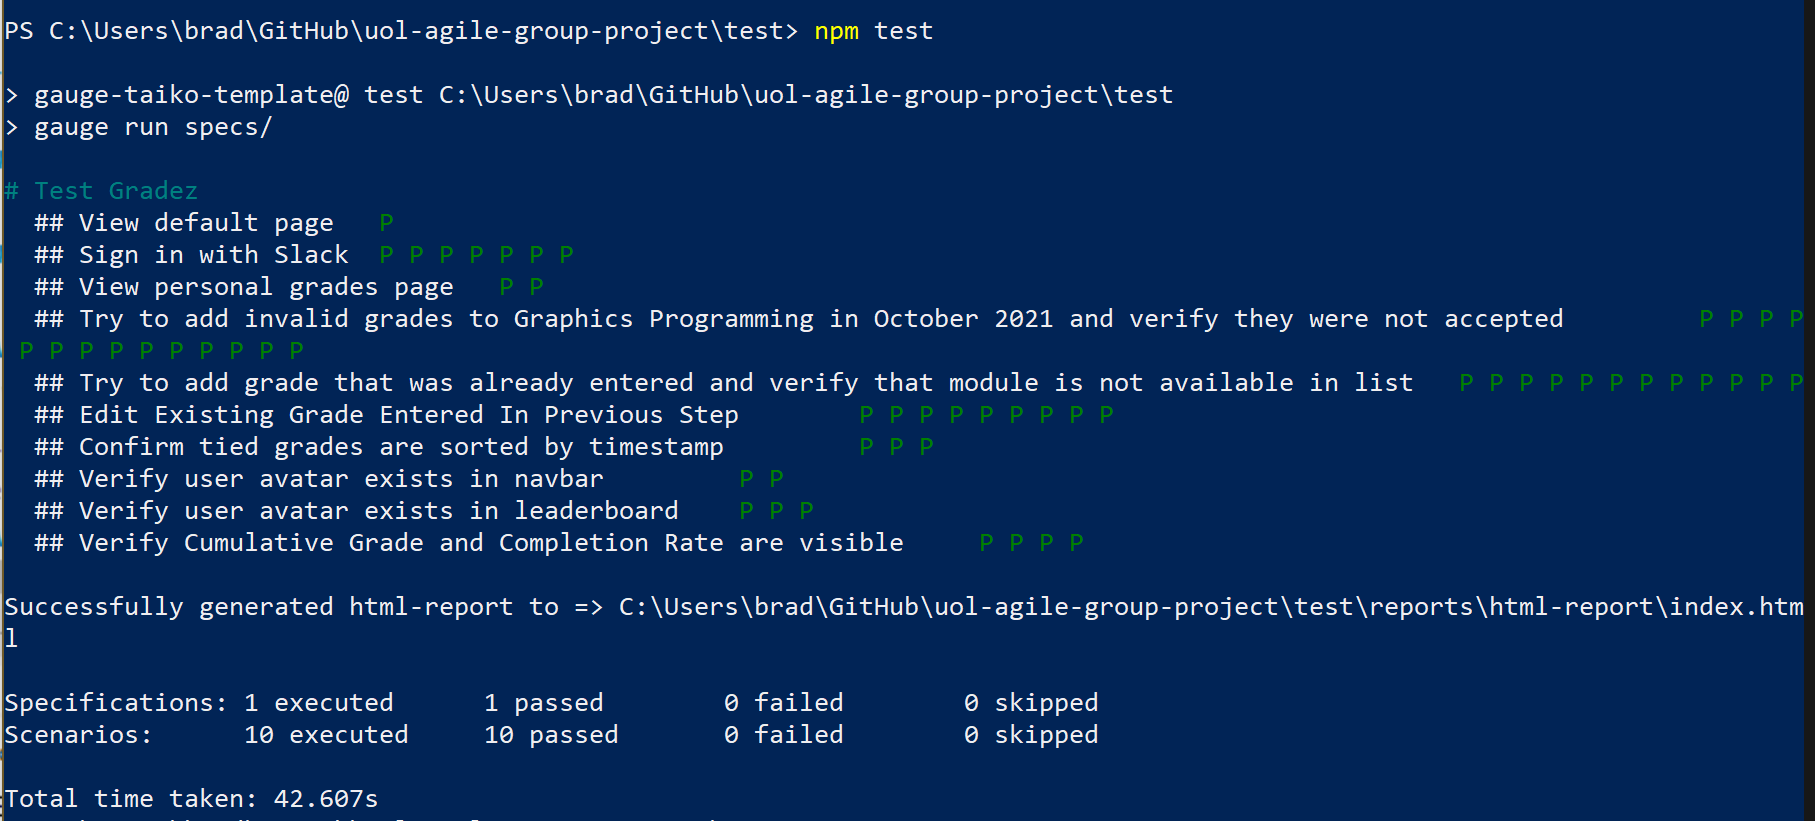
\includegraphics{successful_gauge_testing_log}
\end{figure}

\begin{figure}[H]
	\label{fig:fail_gauge}
	\caption{Failed Gauge Test Log}
	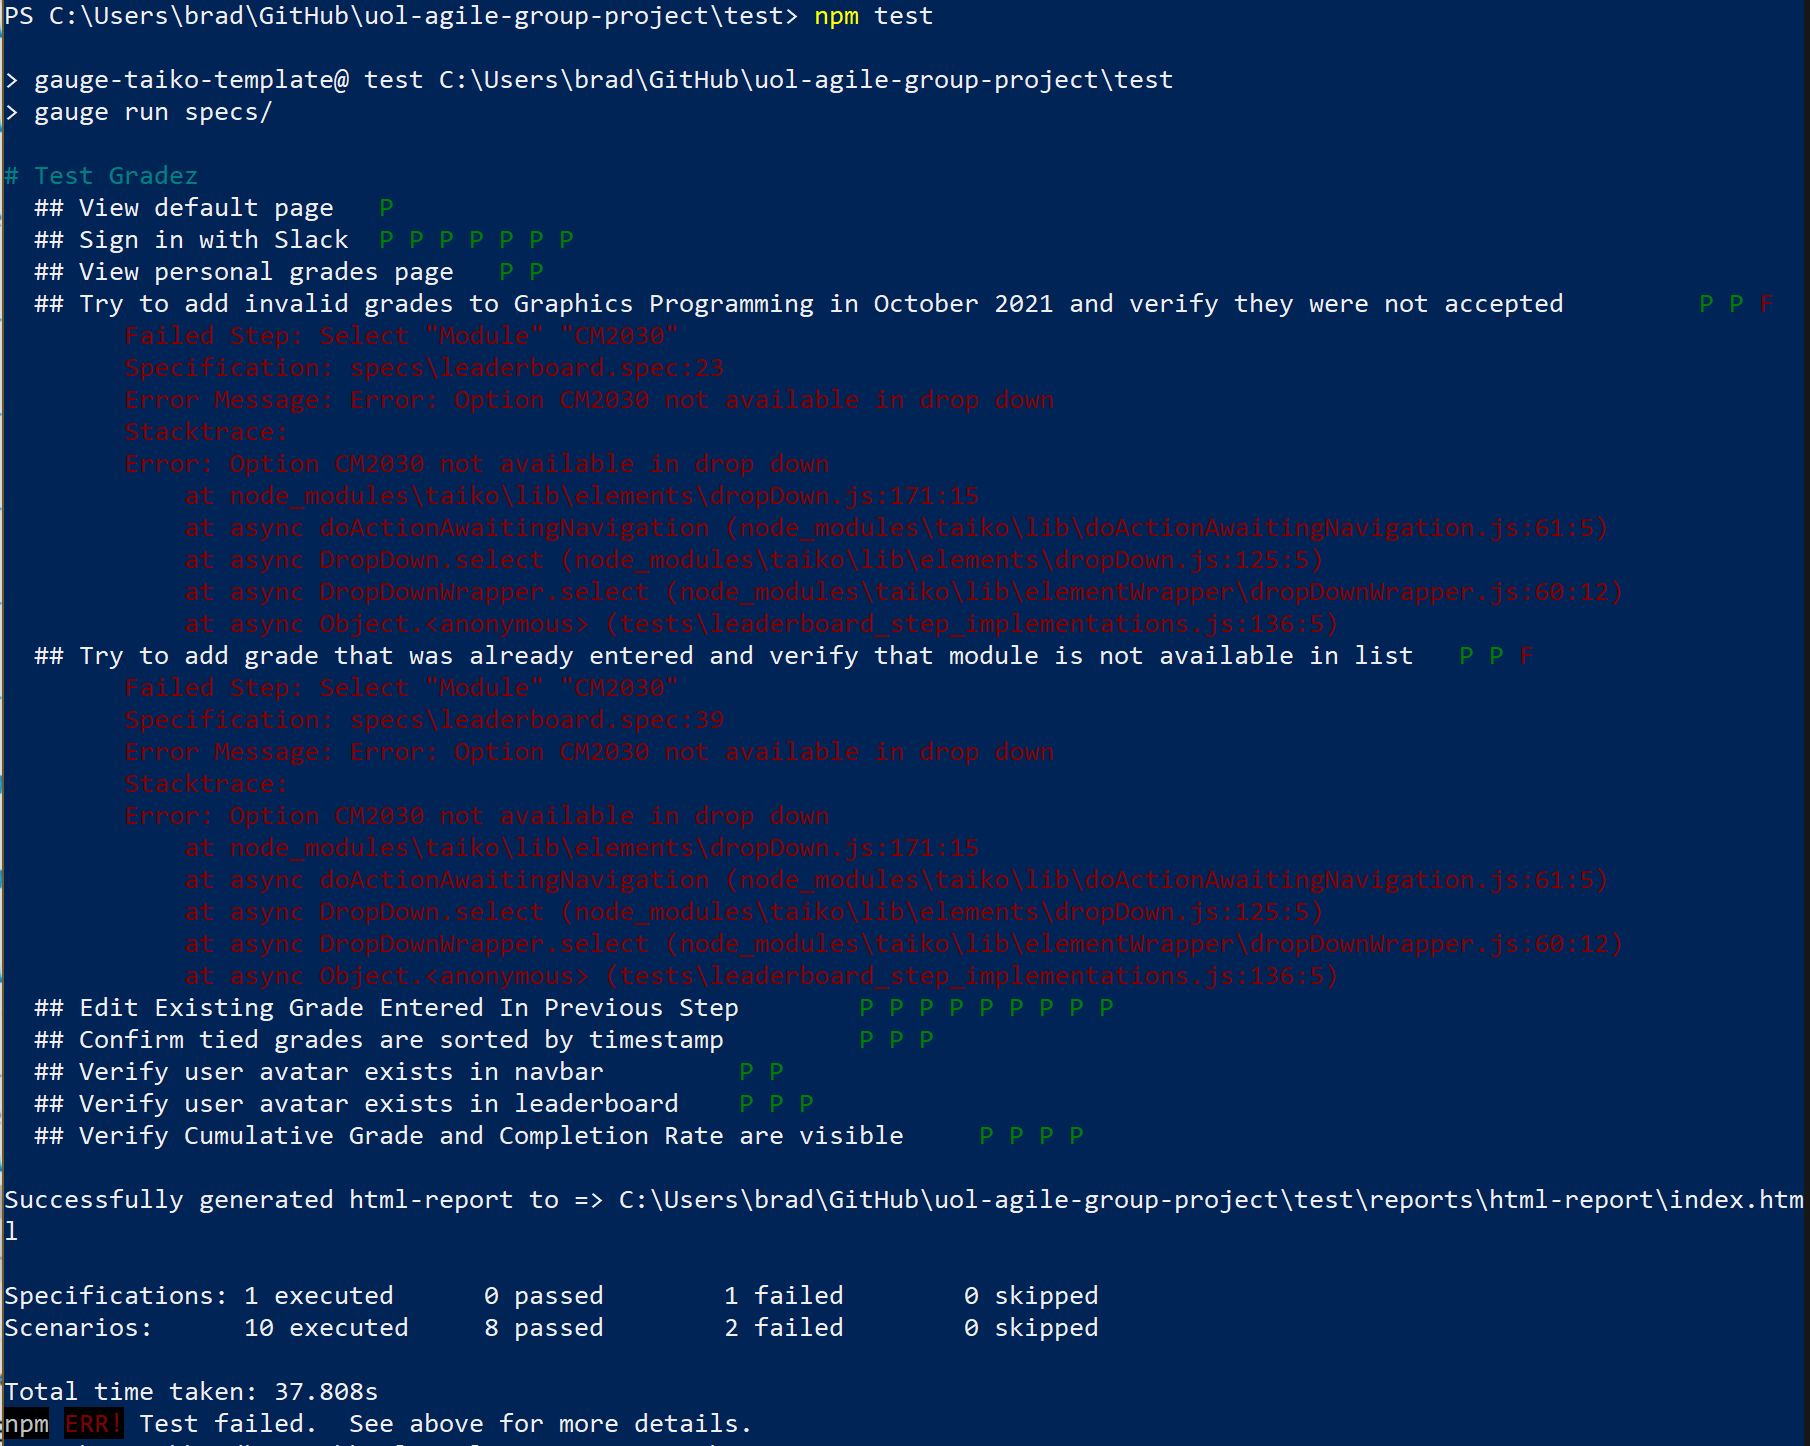
\includegraphics{failed_gauge_testing_log}
\end{figure}

If necessary the software could be configured to show the automated browser window, as shown in \cref{fig:autobrowser}.

\begin{figure}[H]
	\label{fig:autobrowser}
	\caption{Automated Browser Testing}
	
\includegraphics{automated_browser_window_running_tests}
\end{figure}

This allowed the developer to watch as Gauge implemented the Taiko automation steps. Gauge also provides a testing report in HTML format, a sample of which is provided in \cref{fig:success_gauge_testing_report}. 


\begin{figure}[H]
	\label{fig:success_gauge_report}
	\caption{Successful Gauge Testing Report}
	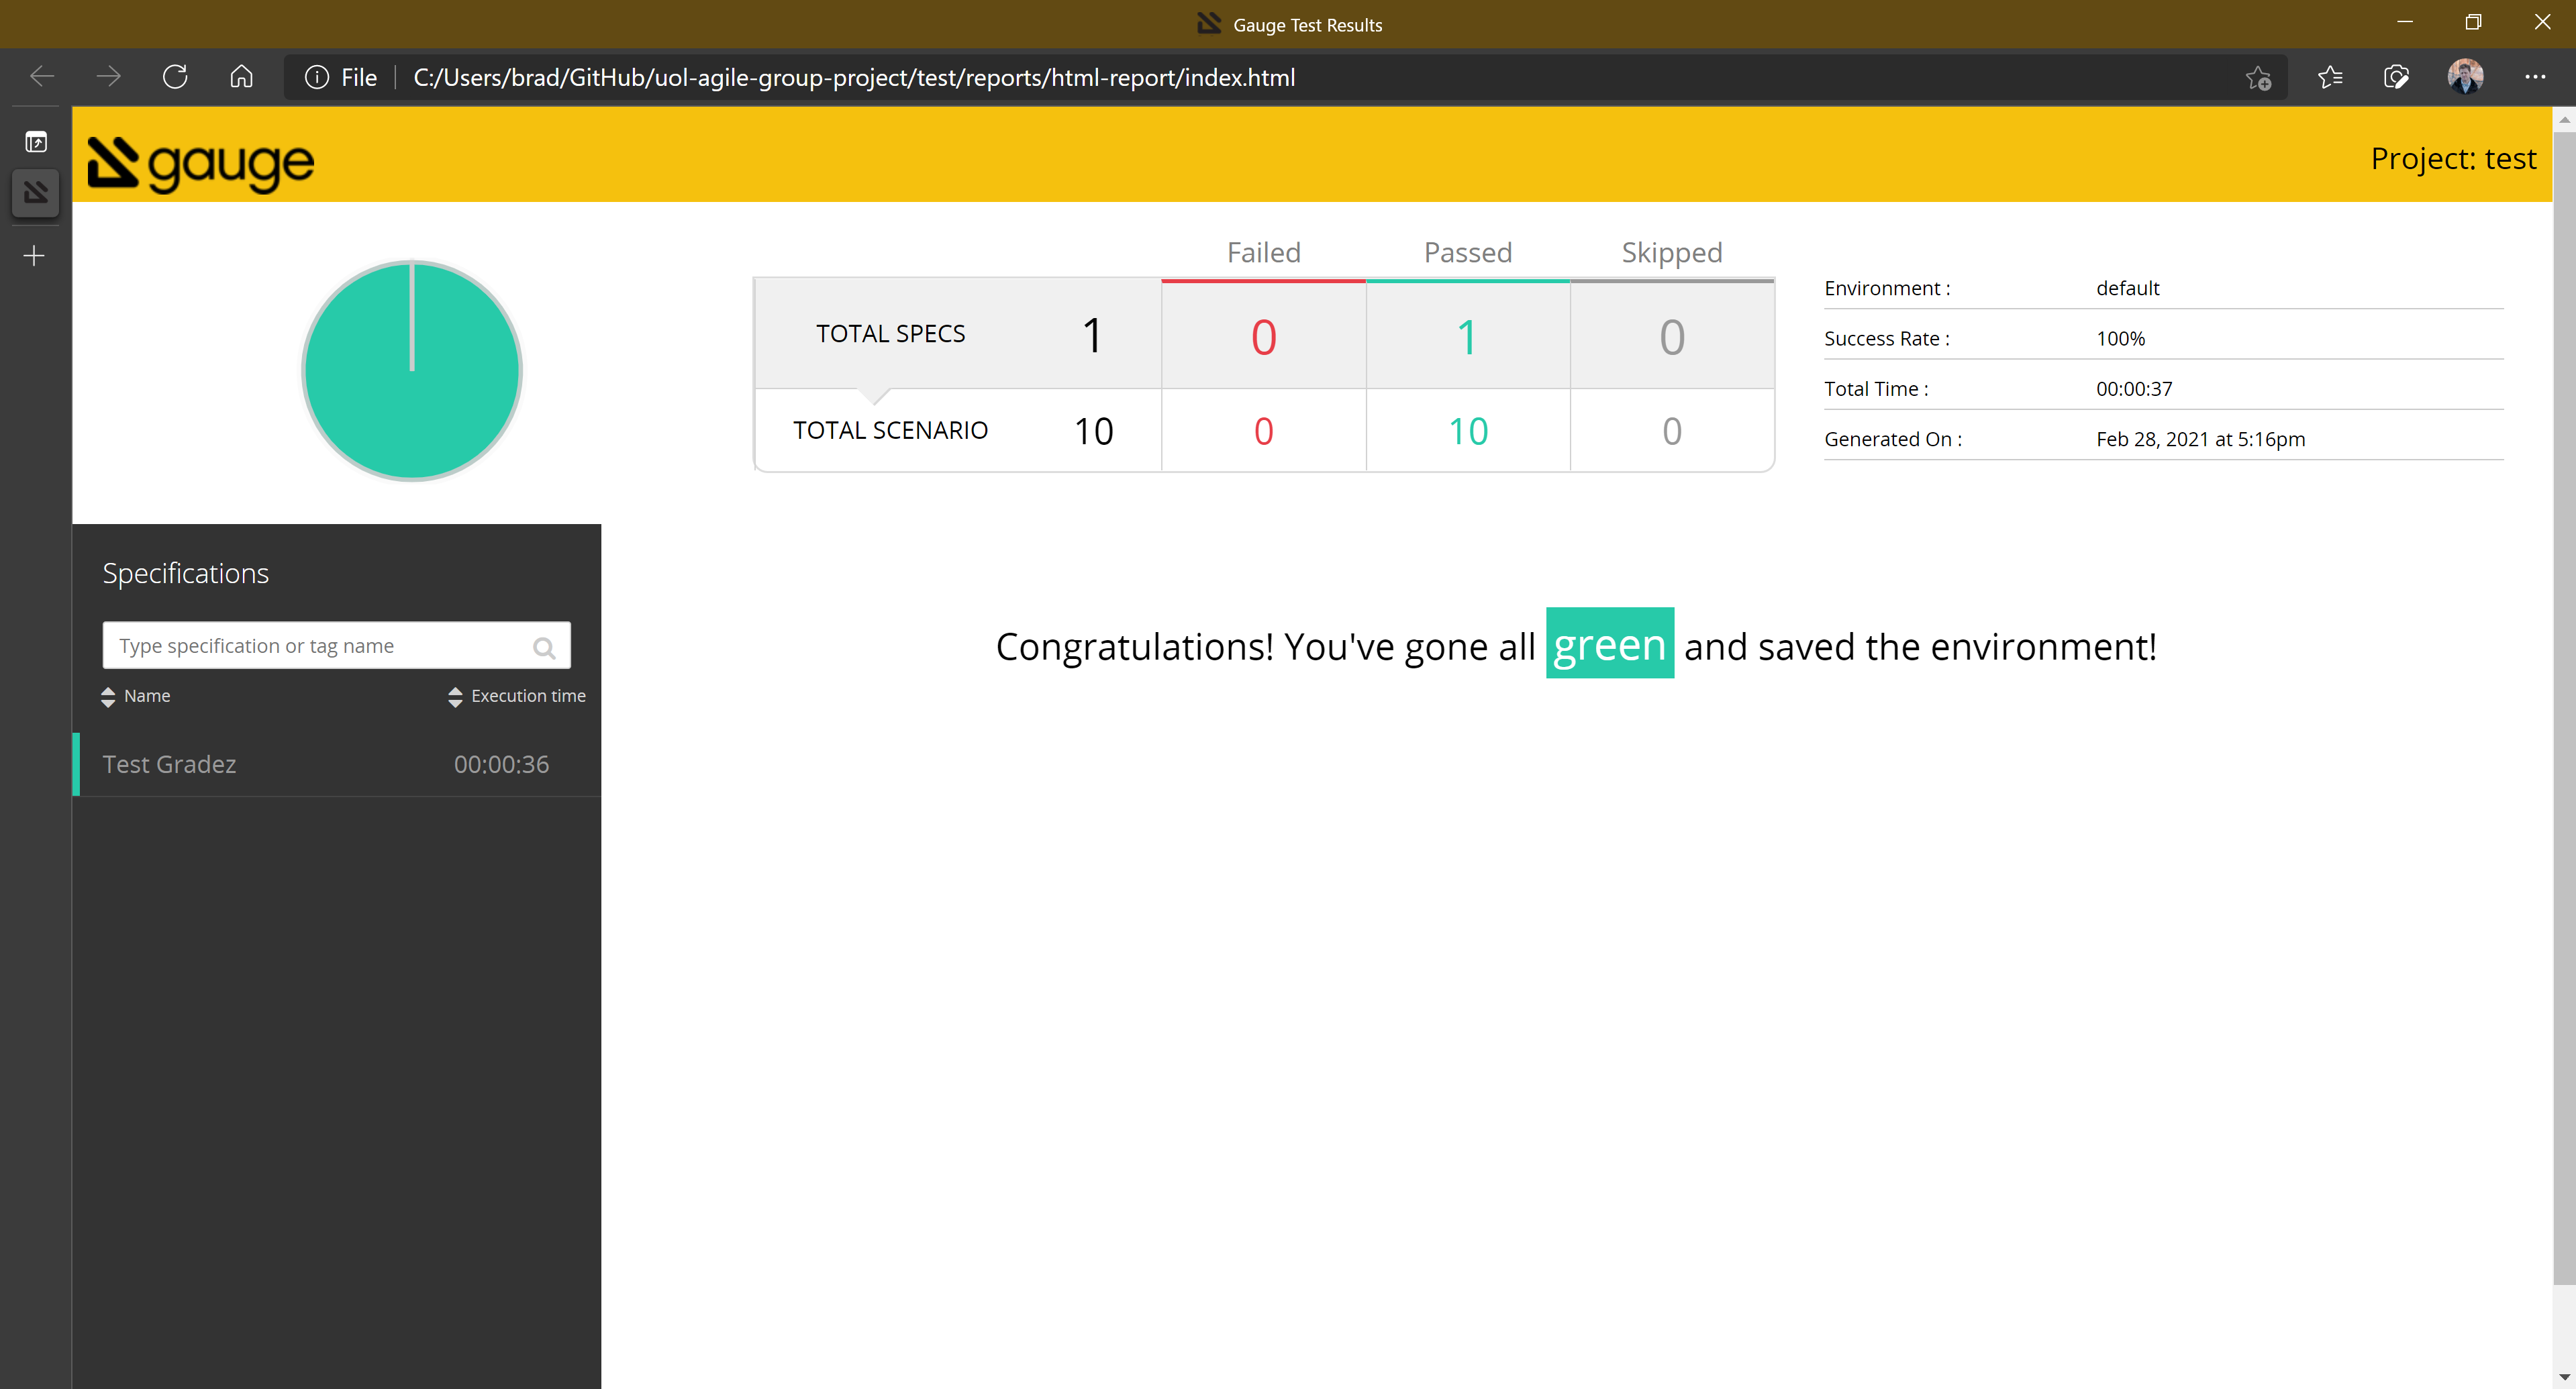
\includegraphics{successful_gauge_testing_report}
\end{figure}

When the testing fails the report indicates this, as shown in \cref{fig:failed_gauge_report}. Additionally Gauge will take screenshots of the automated browser window to aid the developer in determining the cause of the failure, as shown in \cref{fig:failed_gauge_report_detail}.

\begin{figure}[H]
	\label{fig:failed_gauge_report}
	\caption{Failed Gauge Testing Report}
	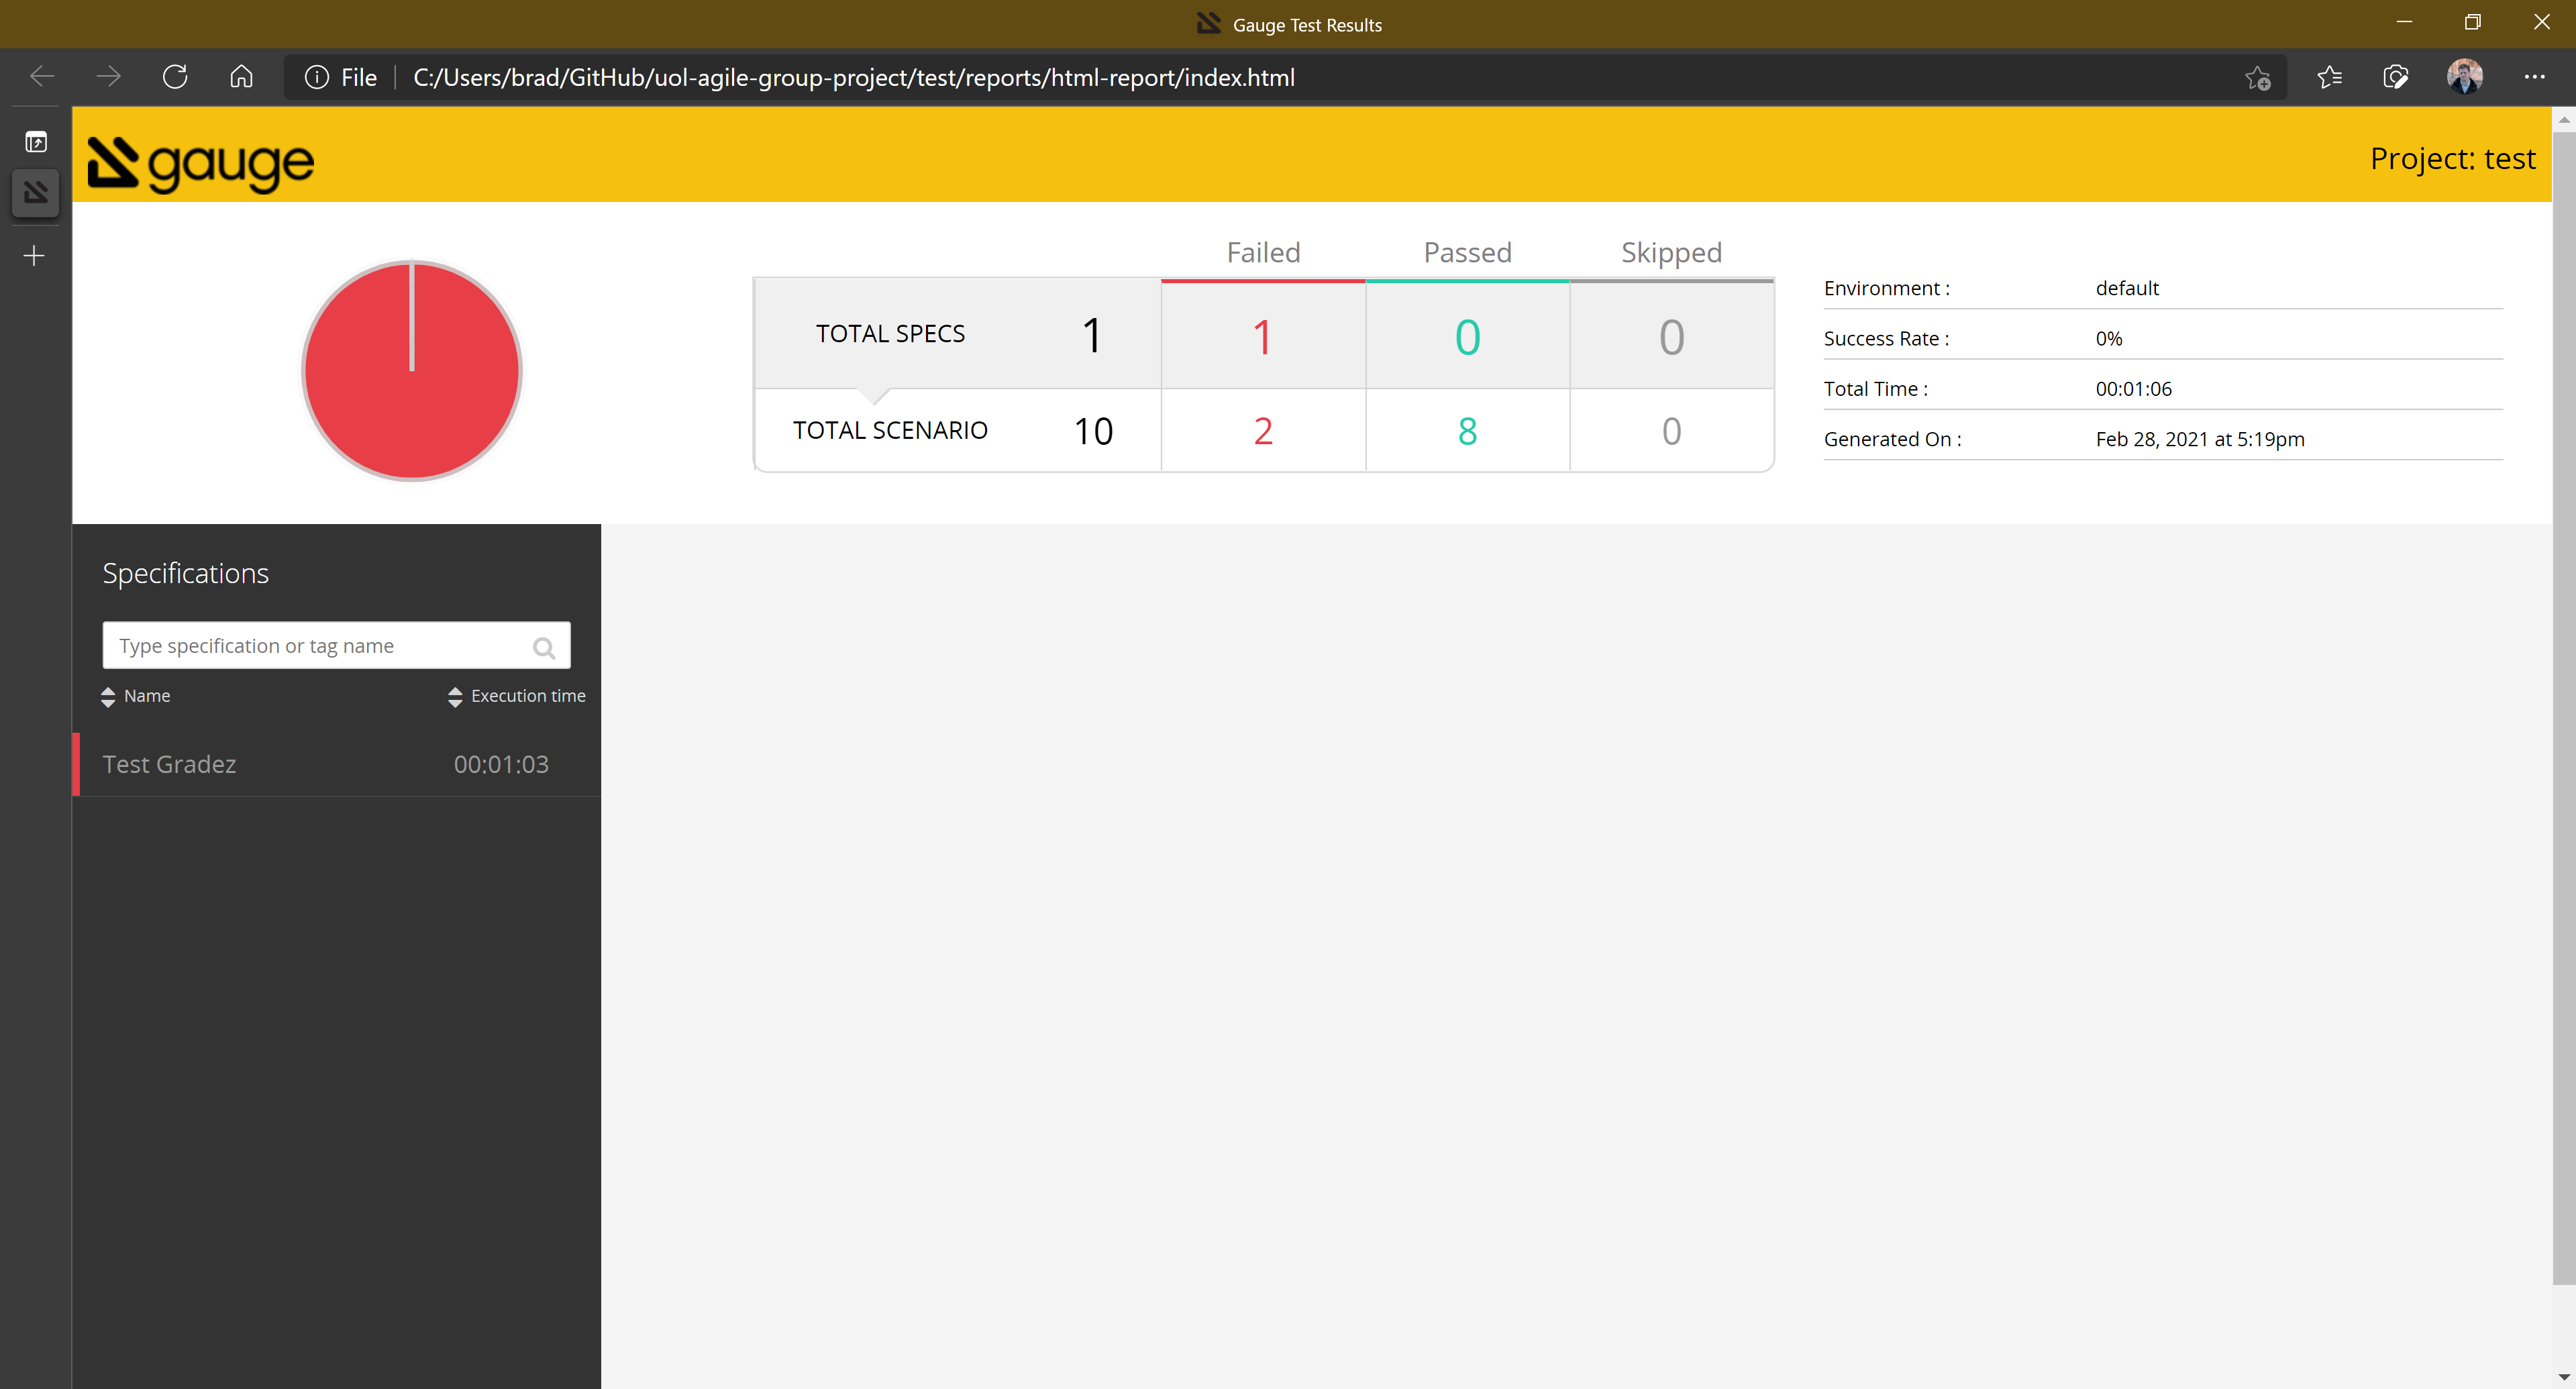
\includegraphics{failed_gauge_testing_report}
\end{figure}

\begin{figure}[H]
	\label{fig:failed_gauge_testing_report_detail}
	\caption{Failed Gauge Testing Report - Detailed View}
	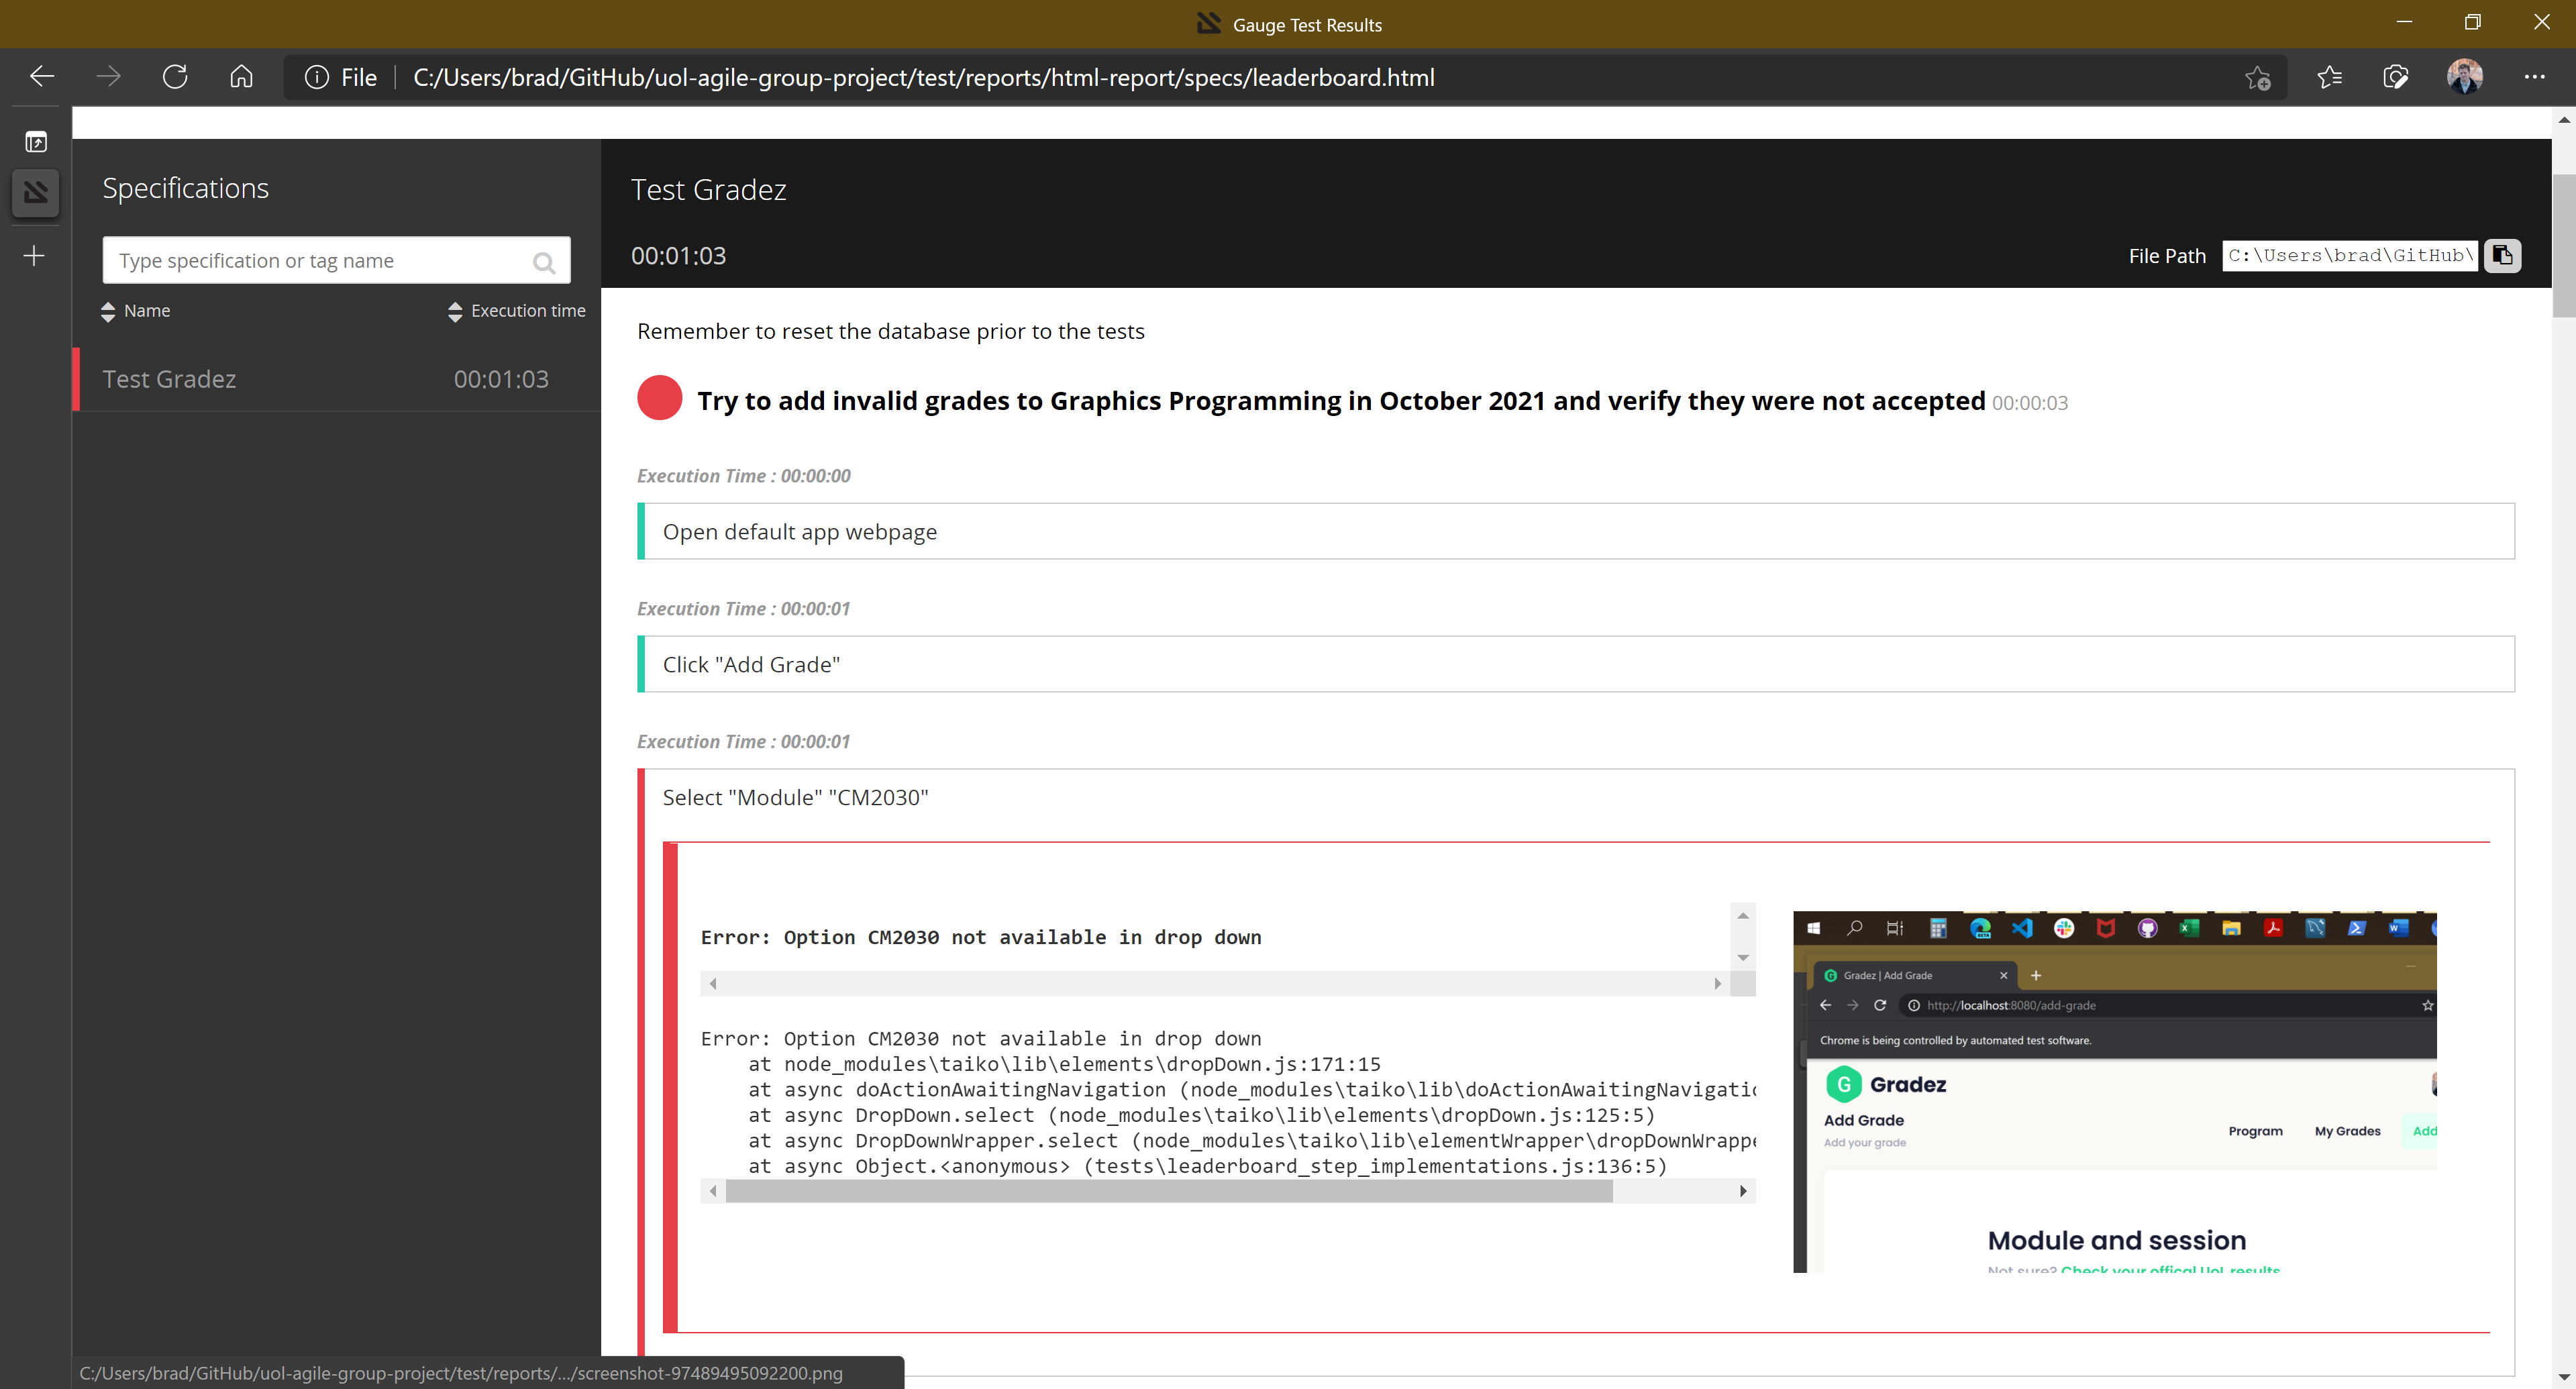
\includegraphics{failed_gauge_testing_report_detail}
\end{figure}

By using the automation testing software we were able to run acceptance tests on the application repeatedly throughout the development process. Additionally by standardizing the tests we removed some of the aspects of human error from the testing by better ensuring that the same tests were run each time. Knowing that the software would provide a quick log and a detailed report in the event of a failure gave us a better sense of confidence that whatever change we were implementing to the code was not causing the application to fail in a way that we were not focusing on at that time.


\subsubsection{User Feedback}

We tested the first iteration of the application with four real-world student users. Test subjects were asked to use the application with basic guidance and record observations, using the previously outlined UMUX-Lite approach. The key learnings from this initial user testing are summarised below, with a full list available in the appendix.

\begin{itemize}
    \item Because pages look similar, some navigational feedback is necessary to indicate where users are. They felt lost.
    \item It wasn't clear what functionality is available to logged in users vs. public users.
    \item It wasn't clear that some grades are anonymous, these need to be marked more clearly and present a default image next to them
    \item The login procedure isn't very friendly to use, and overall the product looks dull and uninviting.
\end{itemize}

A number of smaller usability issues were also mentioned, which we considered as scope for the next iteration. We decided to capture all feedback items and prioritize them by impact and effort for further development.

\subsection{Error Handling}
We have implemented two kinds of error handling in this MVP version of the application. The first is on a technical level, where we have used \texttt{try-catch} blocks in the code, as shown in \cref{lis:trycatch}. This block ensures that a user cannot add a duplicate record to the grades database, and provides a useful error message back to the user. This approach is used throughout the application on all routes.

The UI prevents users from entering a duplicate grade by not offering modules that already have submitted grades. However, we have added an additional layer of error-handling and used the \texttt{try-catch} block to provide a useful error message - in case a user does somehow manage to submit a duplicate grade. Based on \cite{mckay_2013}, we ensured that the button labels are action-oriented and the errors clearly indicate what happened, and what the user can do next.

\begin{listing}[H]
	\caption{Using try-catch blocks for error handling}
	\label{lis:trycatch}
	\begin{minted}{js}
app.post("/addgrade", checkAuth, checkPermission, async (req, res) => {
	try {
		let params = [req.body.course_id, req.body.semester, req.user.id, req.body.grade, !!req.body.anonymous];
		let sql = `
		INSERT INTO grades(course_id, study_session_id, user_id, grade, anonymous)
		VALUES (?, ?, ?, ?, ?)`;
		var [results, _] = await db.query(sql, params);
		res.redirect(req.baseUrl + "?addResult=success");
	} catch (error) {
		console.log(error);
		if (error.code == "ER_DUP_ENTRY") {
			res.redirect(req.baseUrl + `?addResult=You already have a grade for module ${req.body.course_id}. You may edit an existing grade`);
		}
	}
});
	\end{minted}
\end{listing}


\section{System Development}

\subsection{Technical Approach}\label{sec:techapproach}


\subsection{Relevant Code Extracts}\label{sec:code}

% This is a sample block to use for code extracts
\begin{listing}[H]
	\caption{}
	\label{lis:}
	\begin{minted}{js}

	\end{minted}
\end{listing}

\subsection{File Structure}\label{sec:files}
The application uses a file structure as shown in \cref{lis:files}, following a standard pattern for a Node application. The structure separates configuration files, database scripts, middleware (where all the more specific application logic lives), a public folder that contains all the assets need to be served across pages such as images and client-side styling and scripts. Further, the actual application routes are defined in their own folder, and the actual application pages reside in a folder for views.

\begin{listing}[H]
	\caption{}
	\label{lis:files}
	\begin{minted}{text}
TREE
	\end{minted}
\end{listing}

\subsection{Difficulty and novelty of technical challenge}\label{sec:techdiff}
We judged the technical difficulty of this application in terms of the skill levels in the team. We chose an approach that was level-appropriate for the varying backgrounds in the team, and included some additional challenges to learn new skills.

\begin{enumerate}
	\item We introduced a more modern routes logic than we learnt in the program's ``Databases, Networks and the Web'' module, by using promise functions. This was new to most team members.
	\item We used Taiko and Gauge for automated browser testing and behaviour-driven development, which was new to most team members as well.
	\item We used Slack-based authentication which was an additional challenge to handle security aspects and integrate with a third-party authentication API.
	\item Finally, we implemented a complex theming solution that required the team to learn how to incorporate the existing application with a new theming solution.
\end{enumerate}

We chose to use well-documented technical approaches, while the main novelty of the solution lies in the open nature of the application for users, using Slack authentication instead of building a silo, and providing a demo mode for first-time users and graders.


\subsection{Cycle 1 (Sprints 1-3)}\label{sec:cycle1}
Based on the previously defined epics, we captured and worked on first user stories during the first sprint of this cycle. The goal of this cycle was:

\begin{enumerate}
    \item Set up the basic scaffolding for the application
    \item Implement all basic functionality for displaying modules and capturing grades
    \item Ensure use of real-world data in the application
    \item Setting up behaviour-driven unit tests
\end{enumerate}

To achieve this first basic version, we decided to implement the previously defined wireframes using a standard Bootstrap theme, without too much focus on aesthetics and a higher focus on basic usability and functionality.

\subsubsection{Sprints}
We worked in 1-week sprints during most cycles and made sure to measure our sprint progress using the SCRUM methodology. We estimated captured user stories, planned them in and worked on the defined scope, tracking our progress using burndown charts. The first three sprints can be seen in \cref{fig:sprint1}, \cref{fig:sprint2} and \cref{fig:sprint3}. 

\begin{figure}[H]
    \centering
    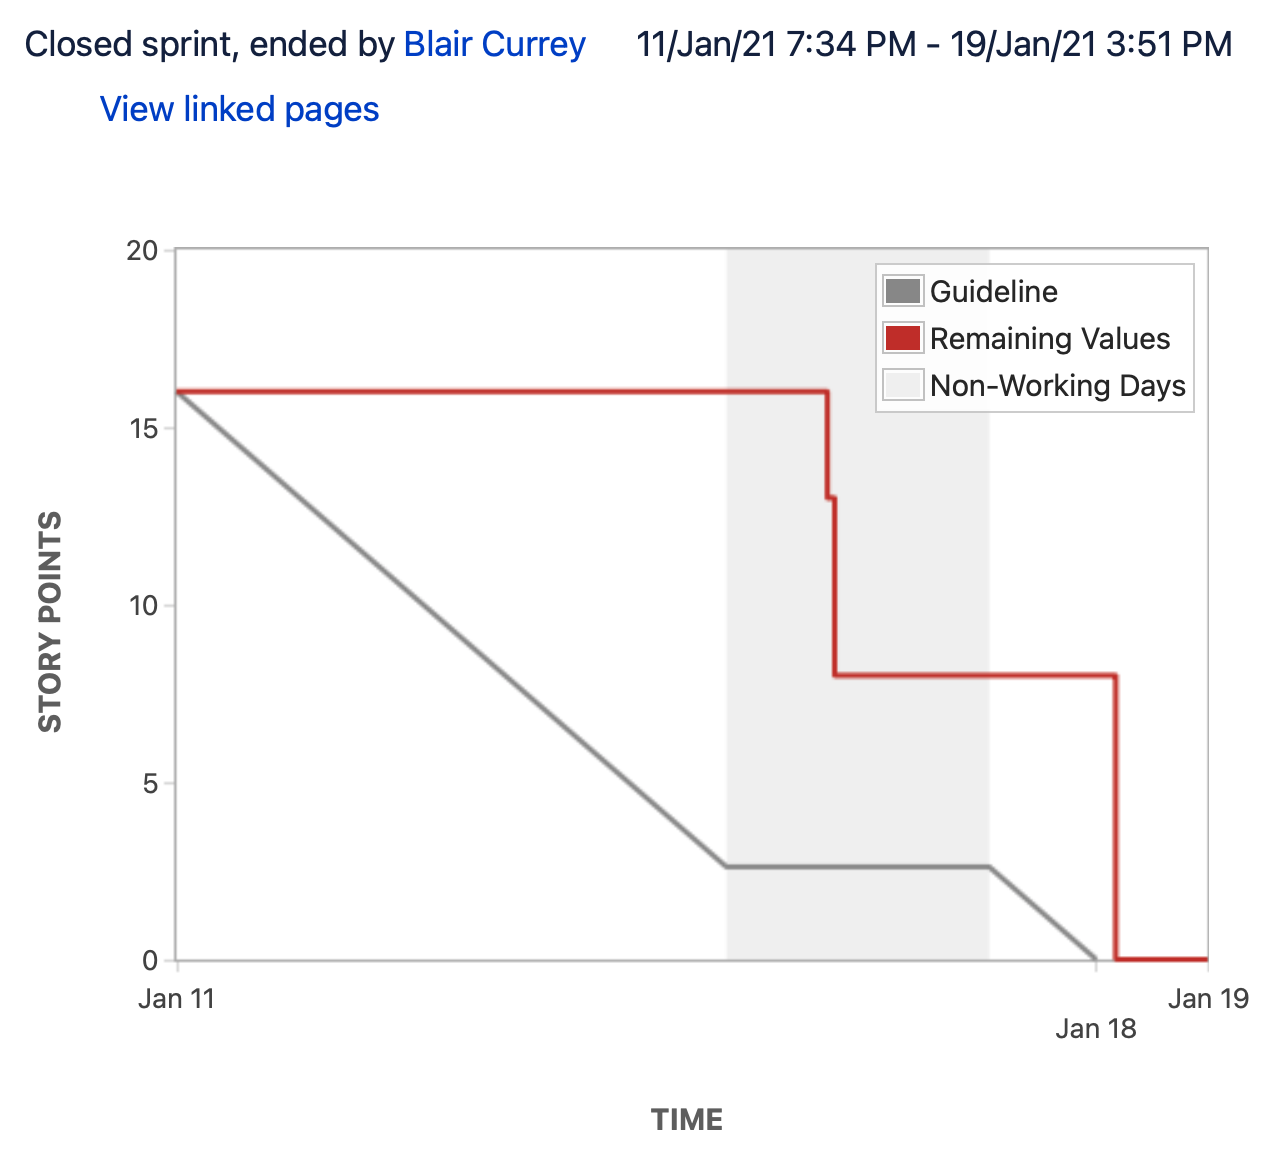
\includegraphics[width=10cm]{images/sprint1.png}
    \caption{Burndown chart - Sprint 1}
    \label{fig:sprint1}
\end{figure}

\begin{figure}[H]
    \centering
    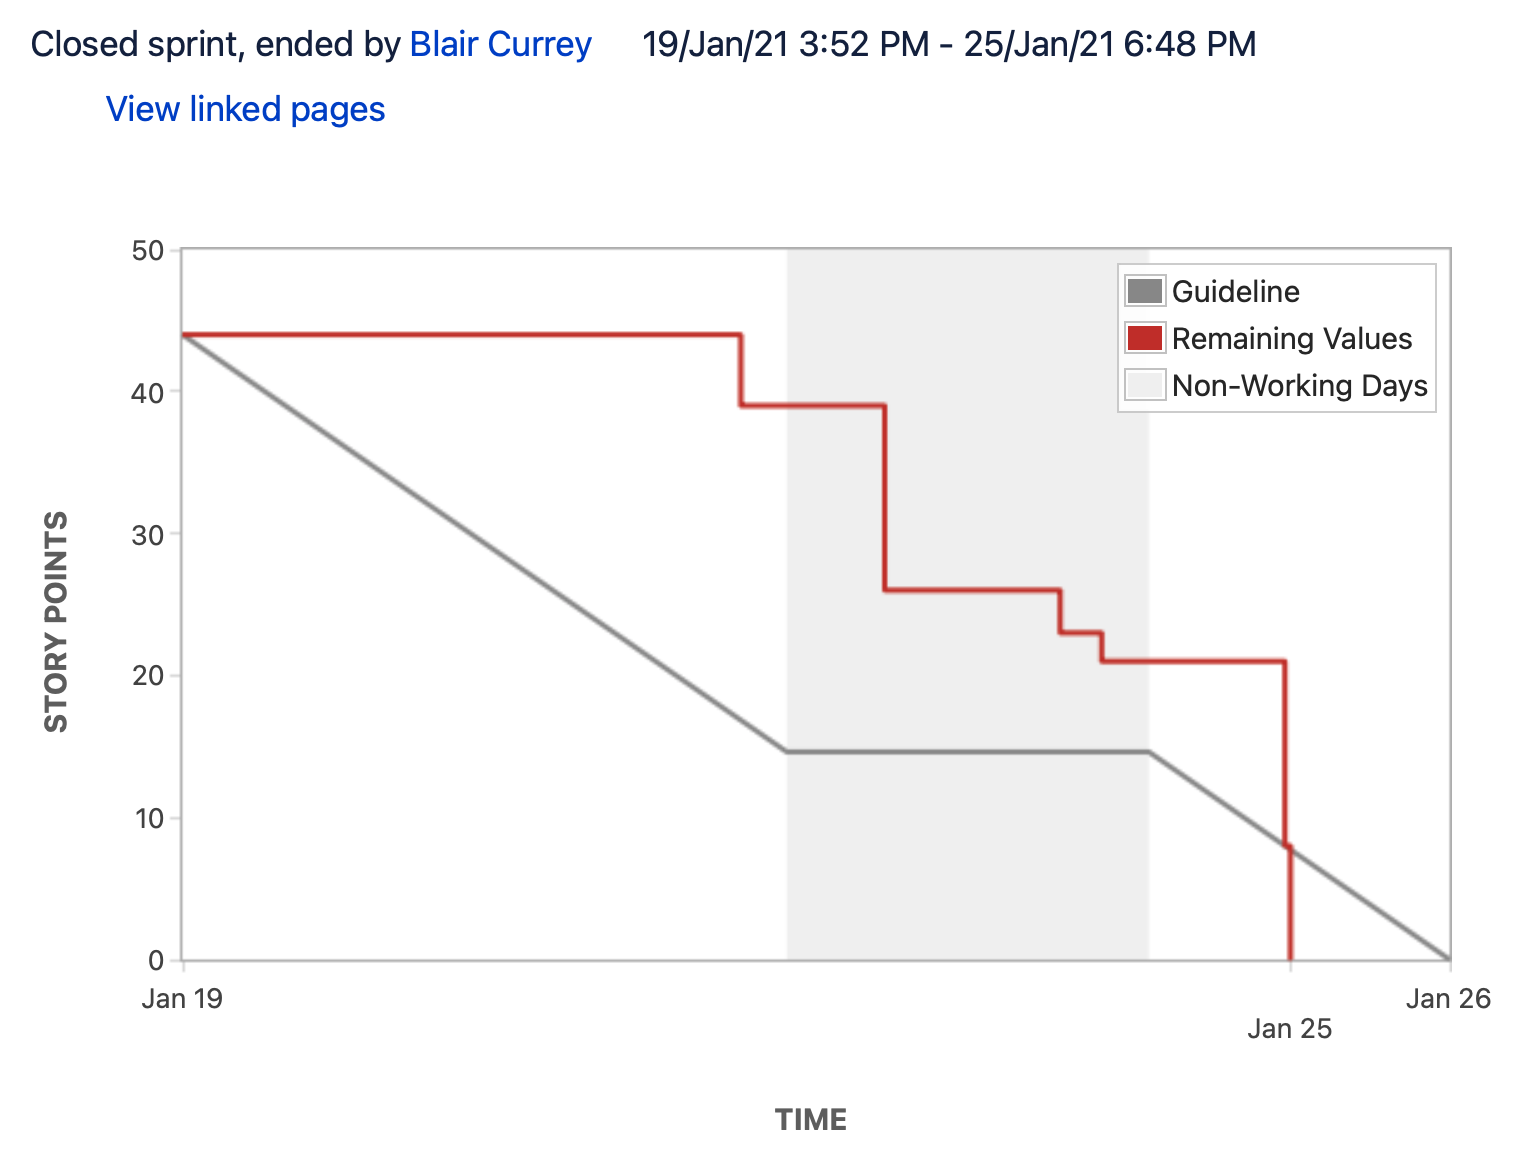
\includegraphics[width=10cm]{images/sprint2.png}
    \caption{Burndown chart - Sprint 2}
    \label{fig:sprint2}
\end{figure}

\begin{figure}[H]
    \centering
    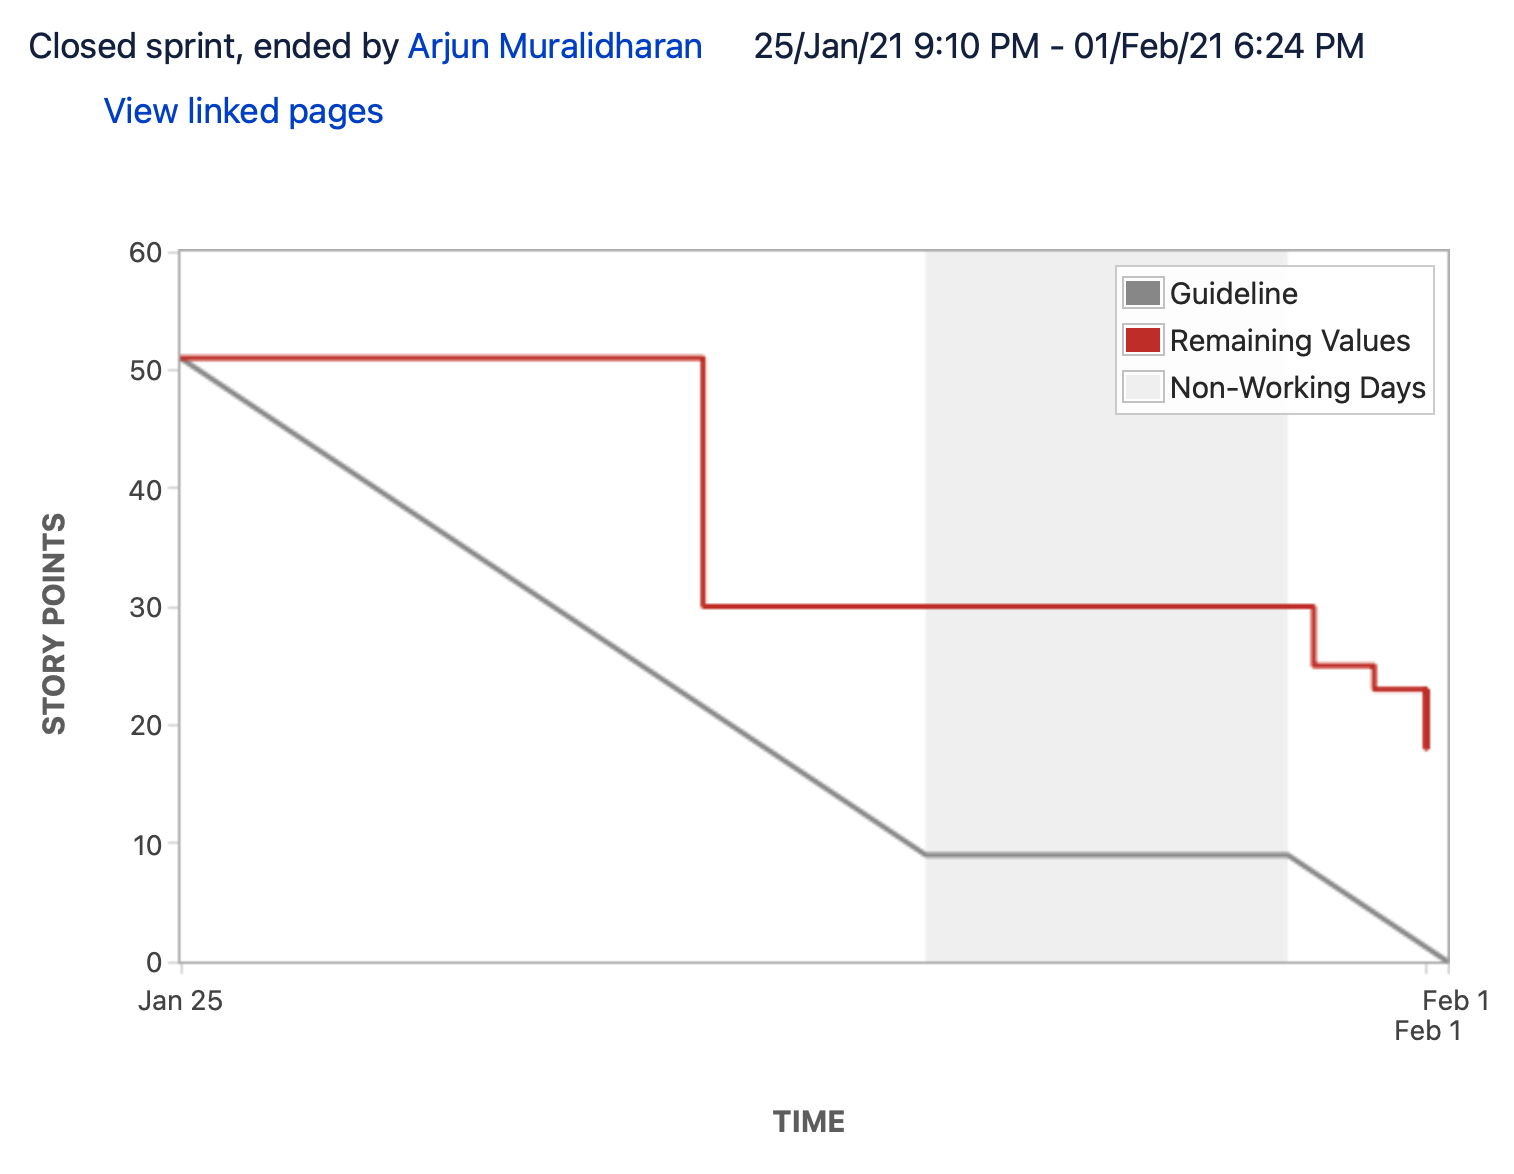
\includegraphics[width=10cm]{images/sprint3.png}
    \caption{Burndown chart - Sprint 3}
    \label{fig:sprint3}
\end{figure}

\subsection{Shipped Product Increment}
At the end of this cycle, we had implemented a functioning version of the grades leaderboard, covering the related user stories (see Appendix A for a list). 

The outcome is shown in \cref{fig:moduleoverview}, \cref{fig:module}, \cref{fig:personal} and \cref{fig:addgrade}.

\begin{figure}[H]
    \centering
    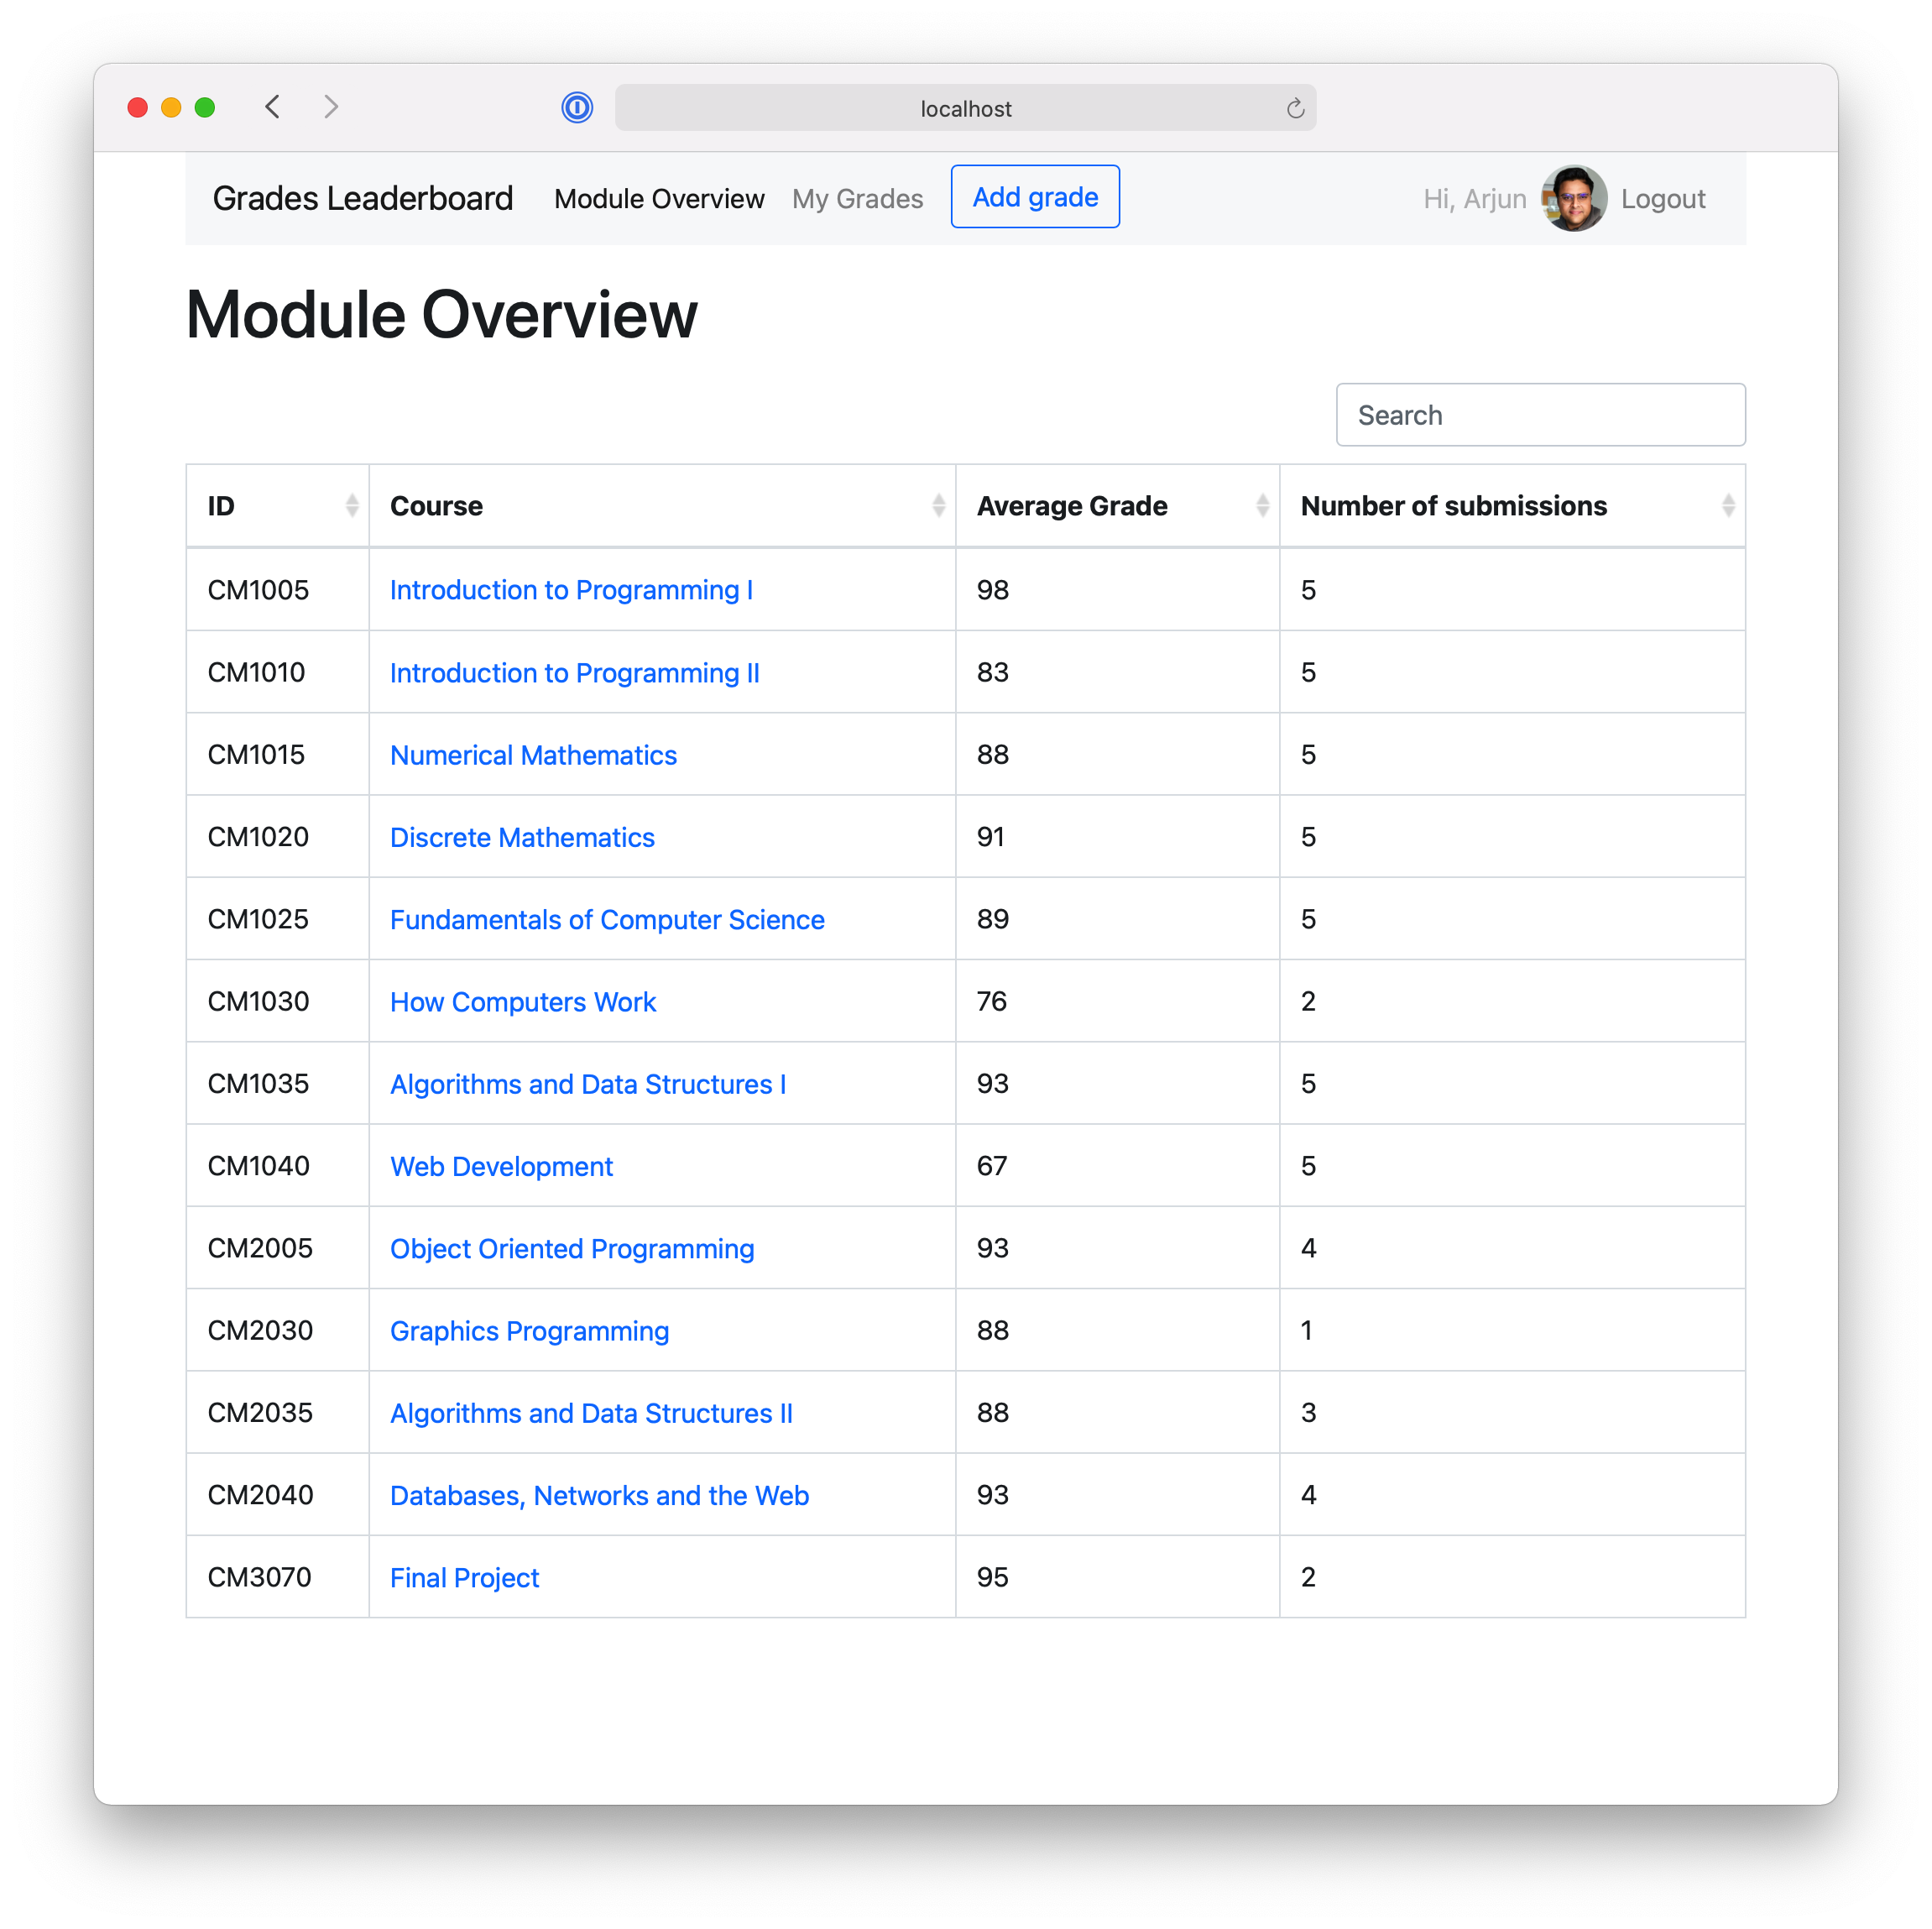
\includegraphics[width=15cm]{images/moduleoverview.png}
    \caption{Module Overview}
    \label{fig:moduleoverview}
\end{figure}

\begin{figure}[H]
    \centering
    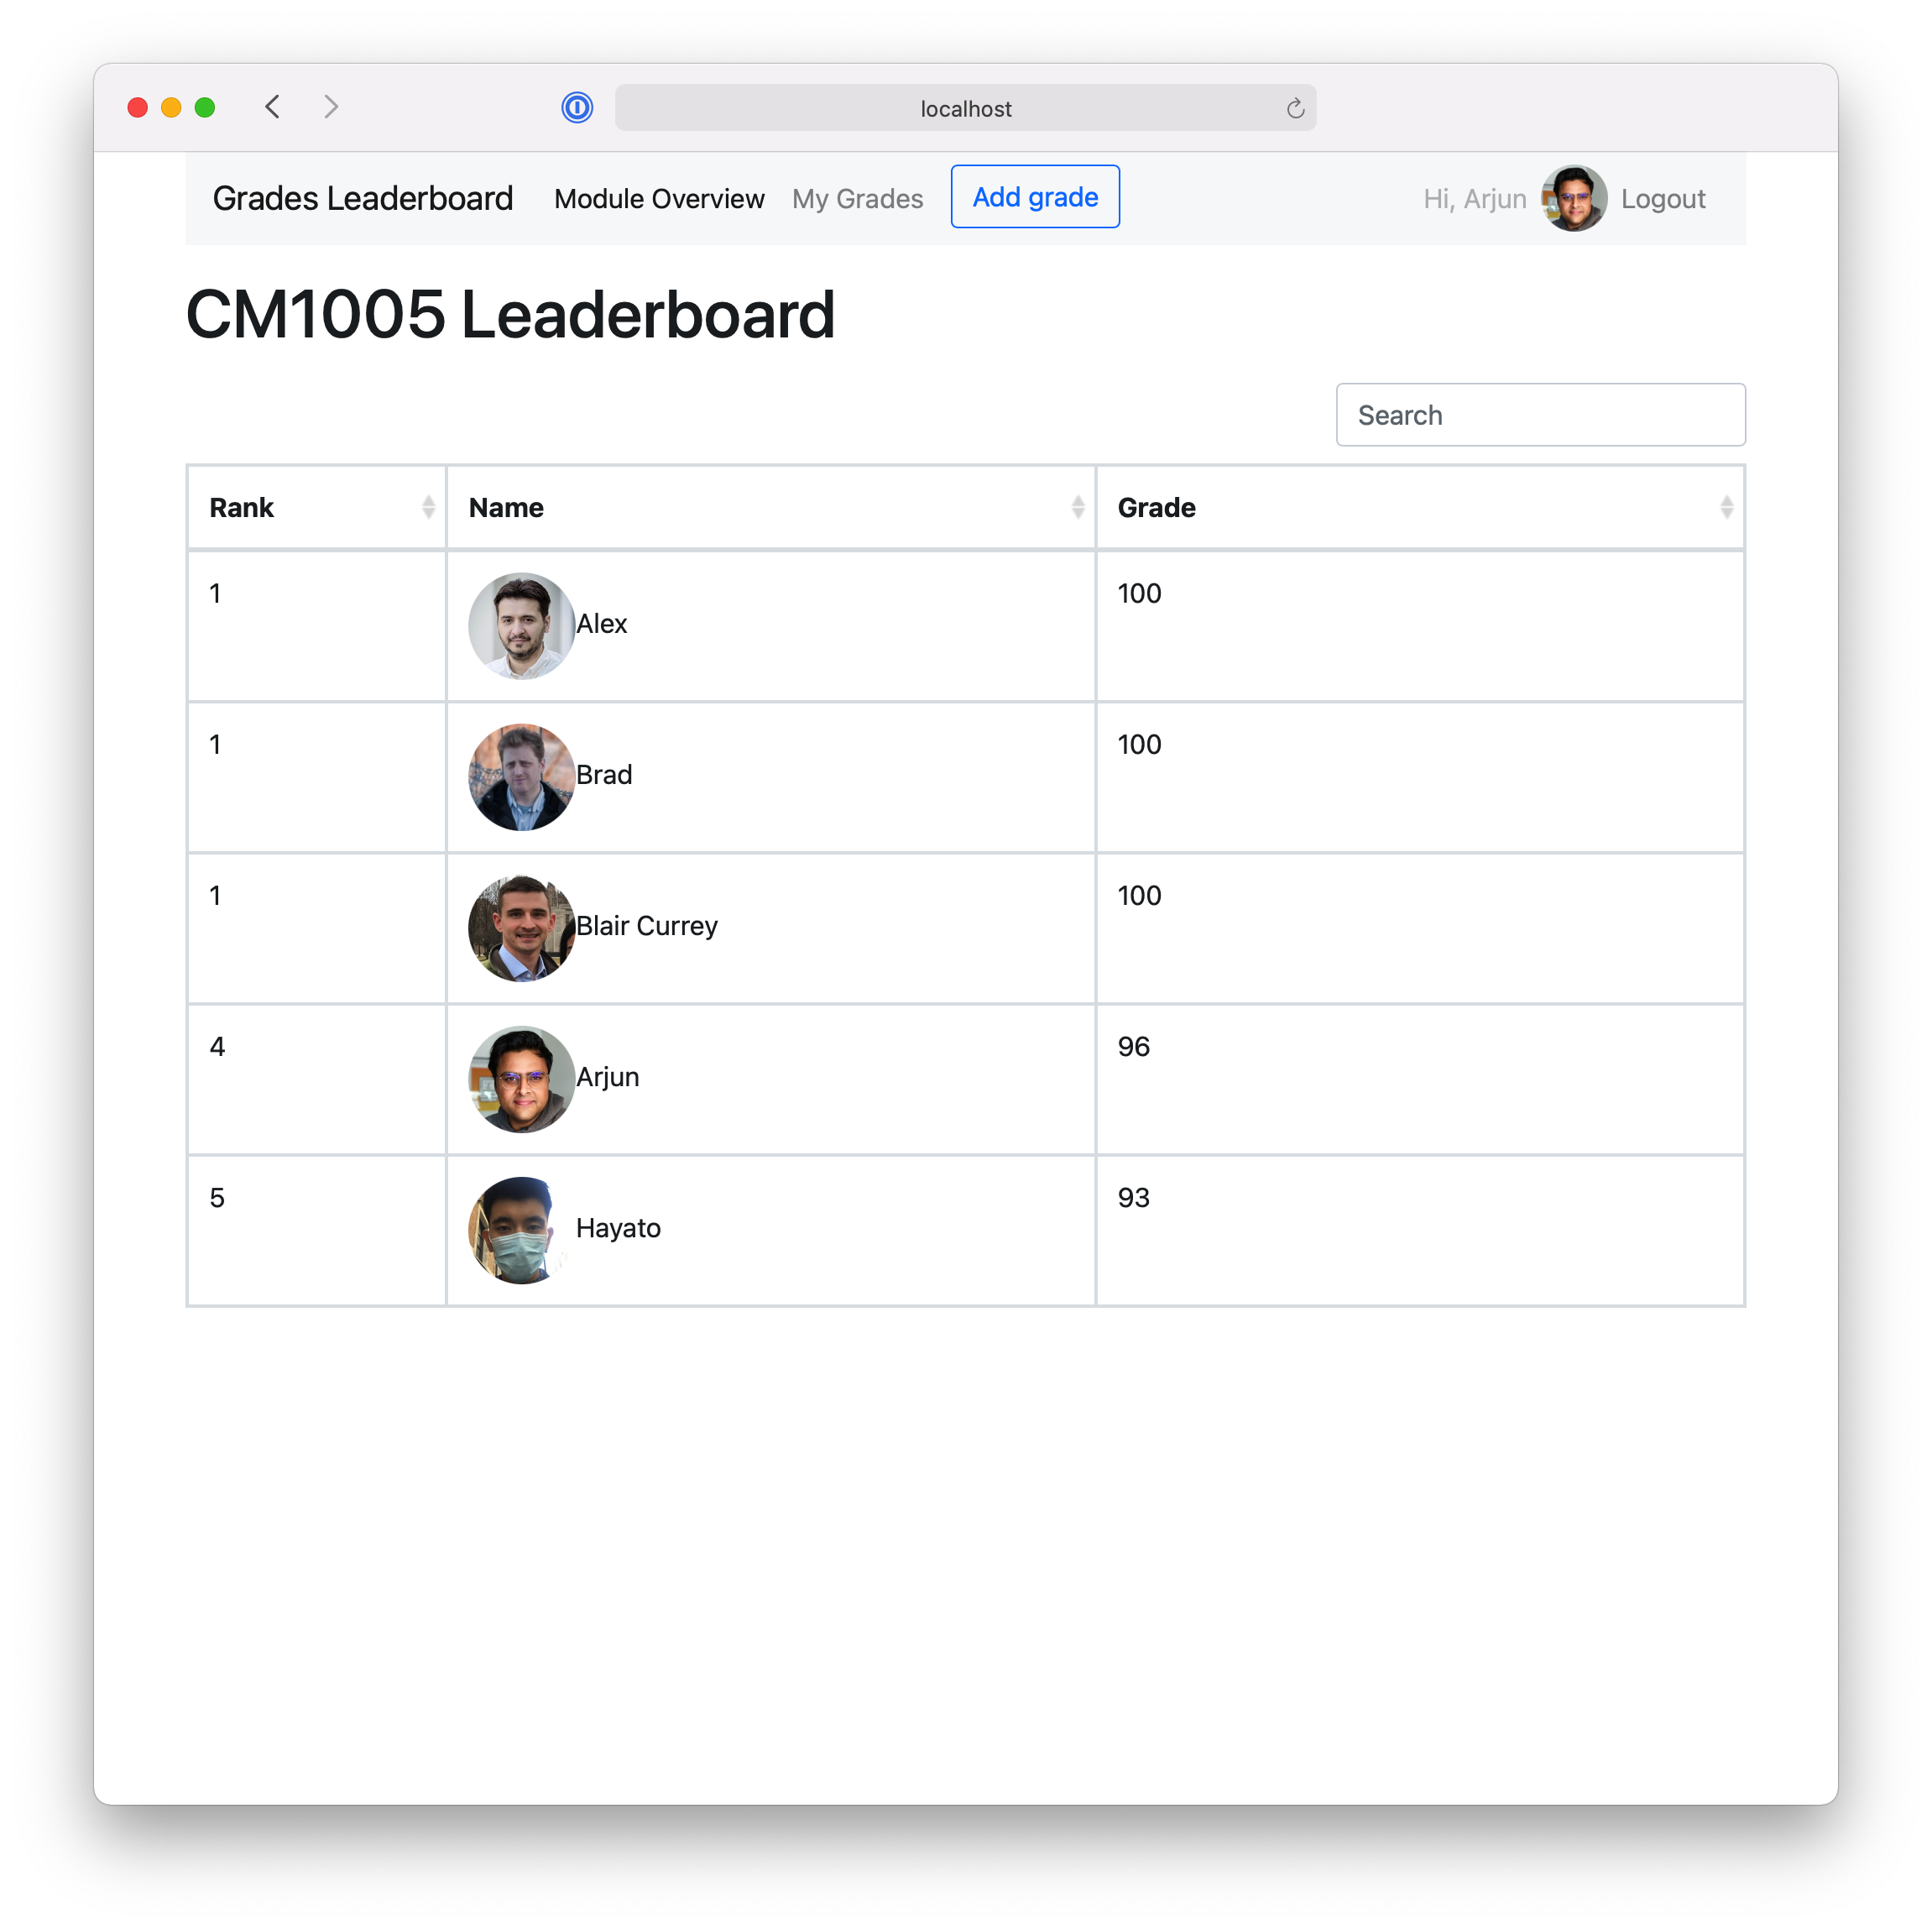
\includegraphics[width=10cm]{images/module.png}
    \caption{Single Module}
    \label{fig:module}
\end{figure}

\begin{figure}[H]
    \centering
    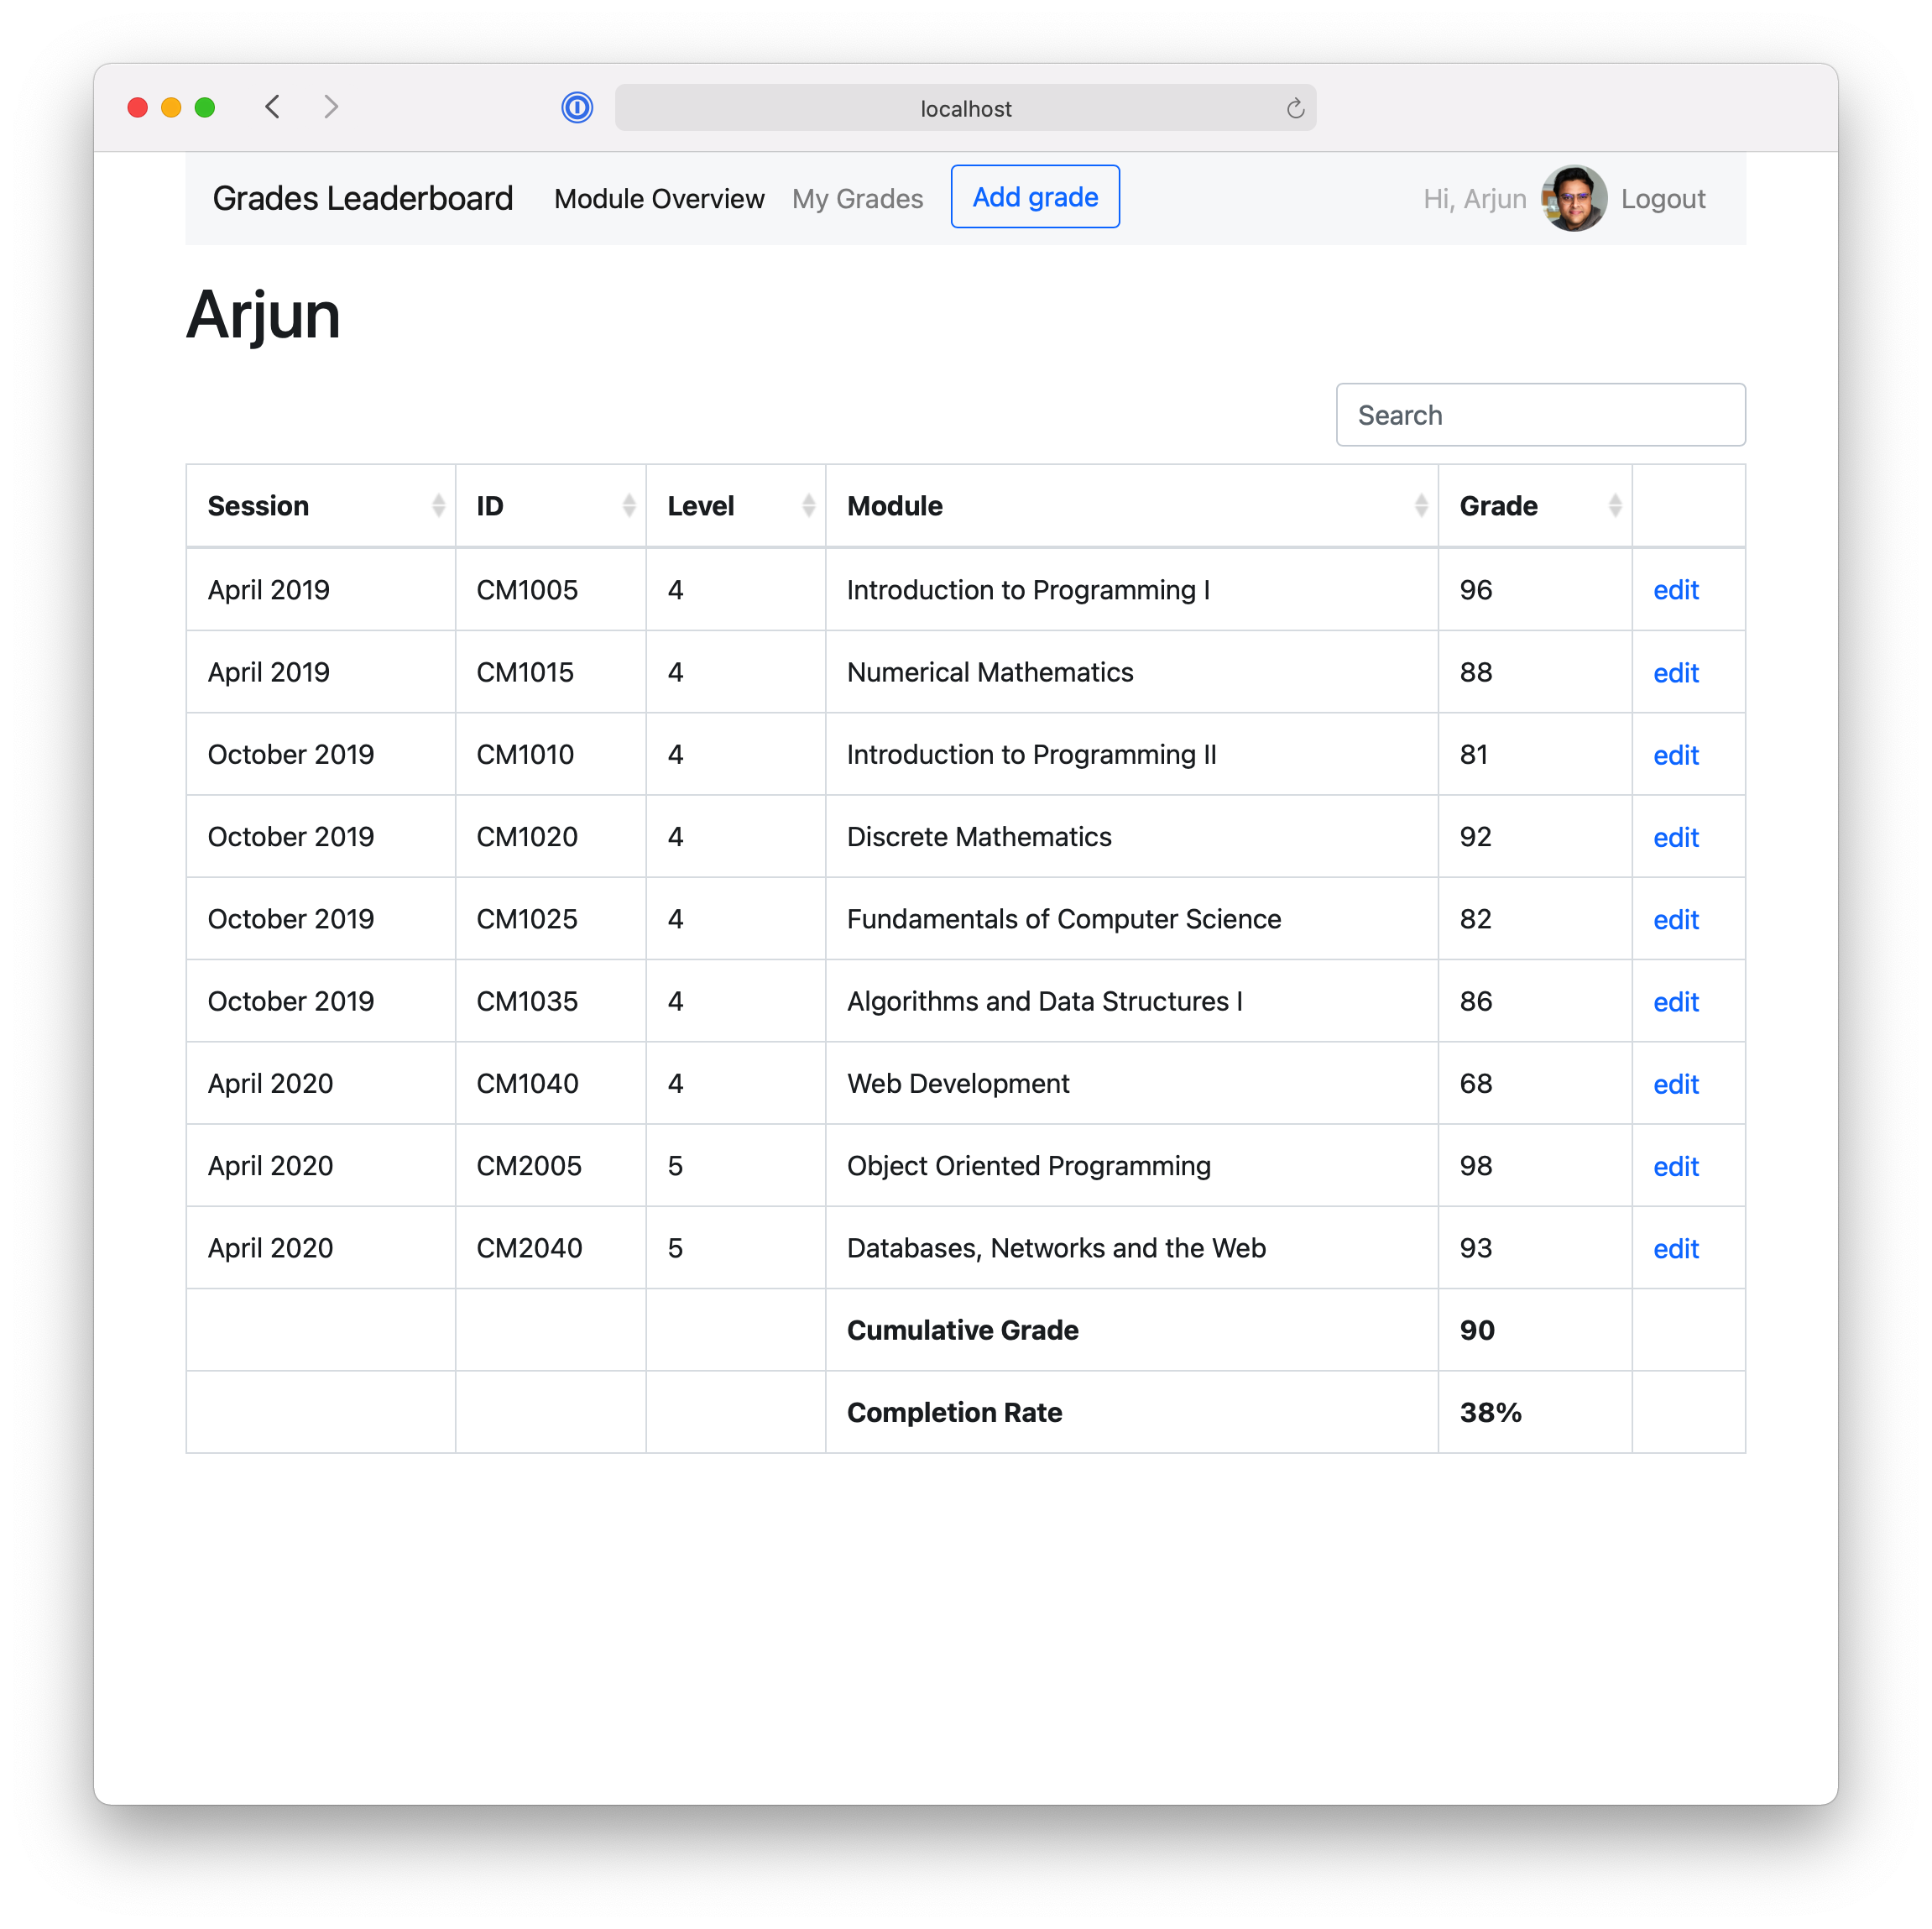
\includegraphics[width=10cm]{images/personal.png}
    \caption{Personal Grades}
    \label{fig:personal}
\end{figure}

\begin{figure}[H]
    \centering
    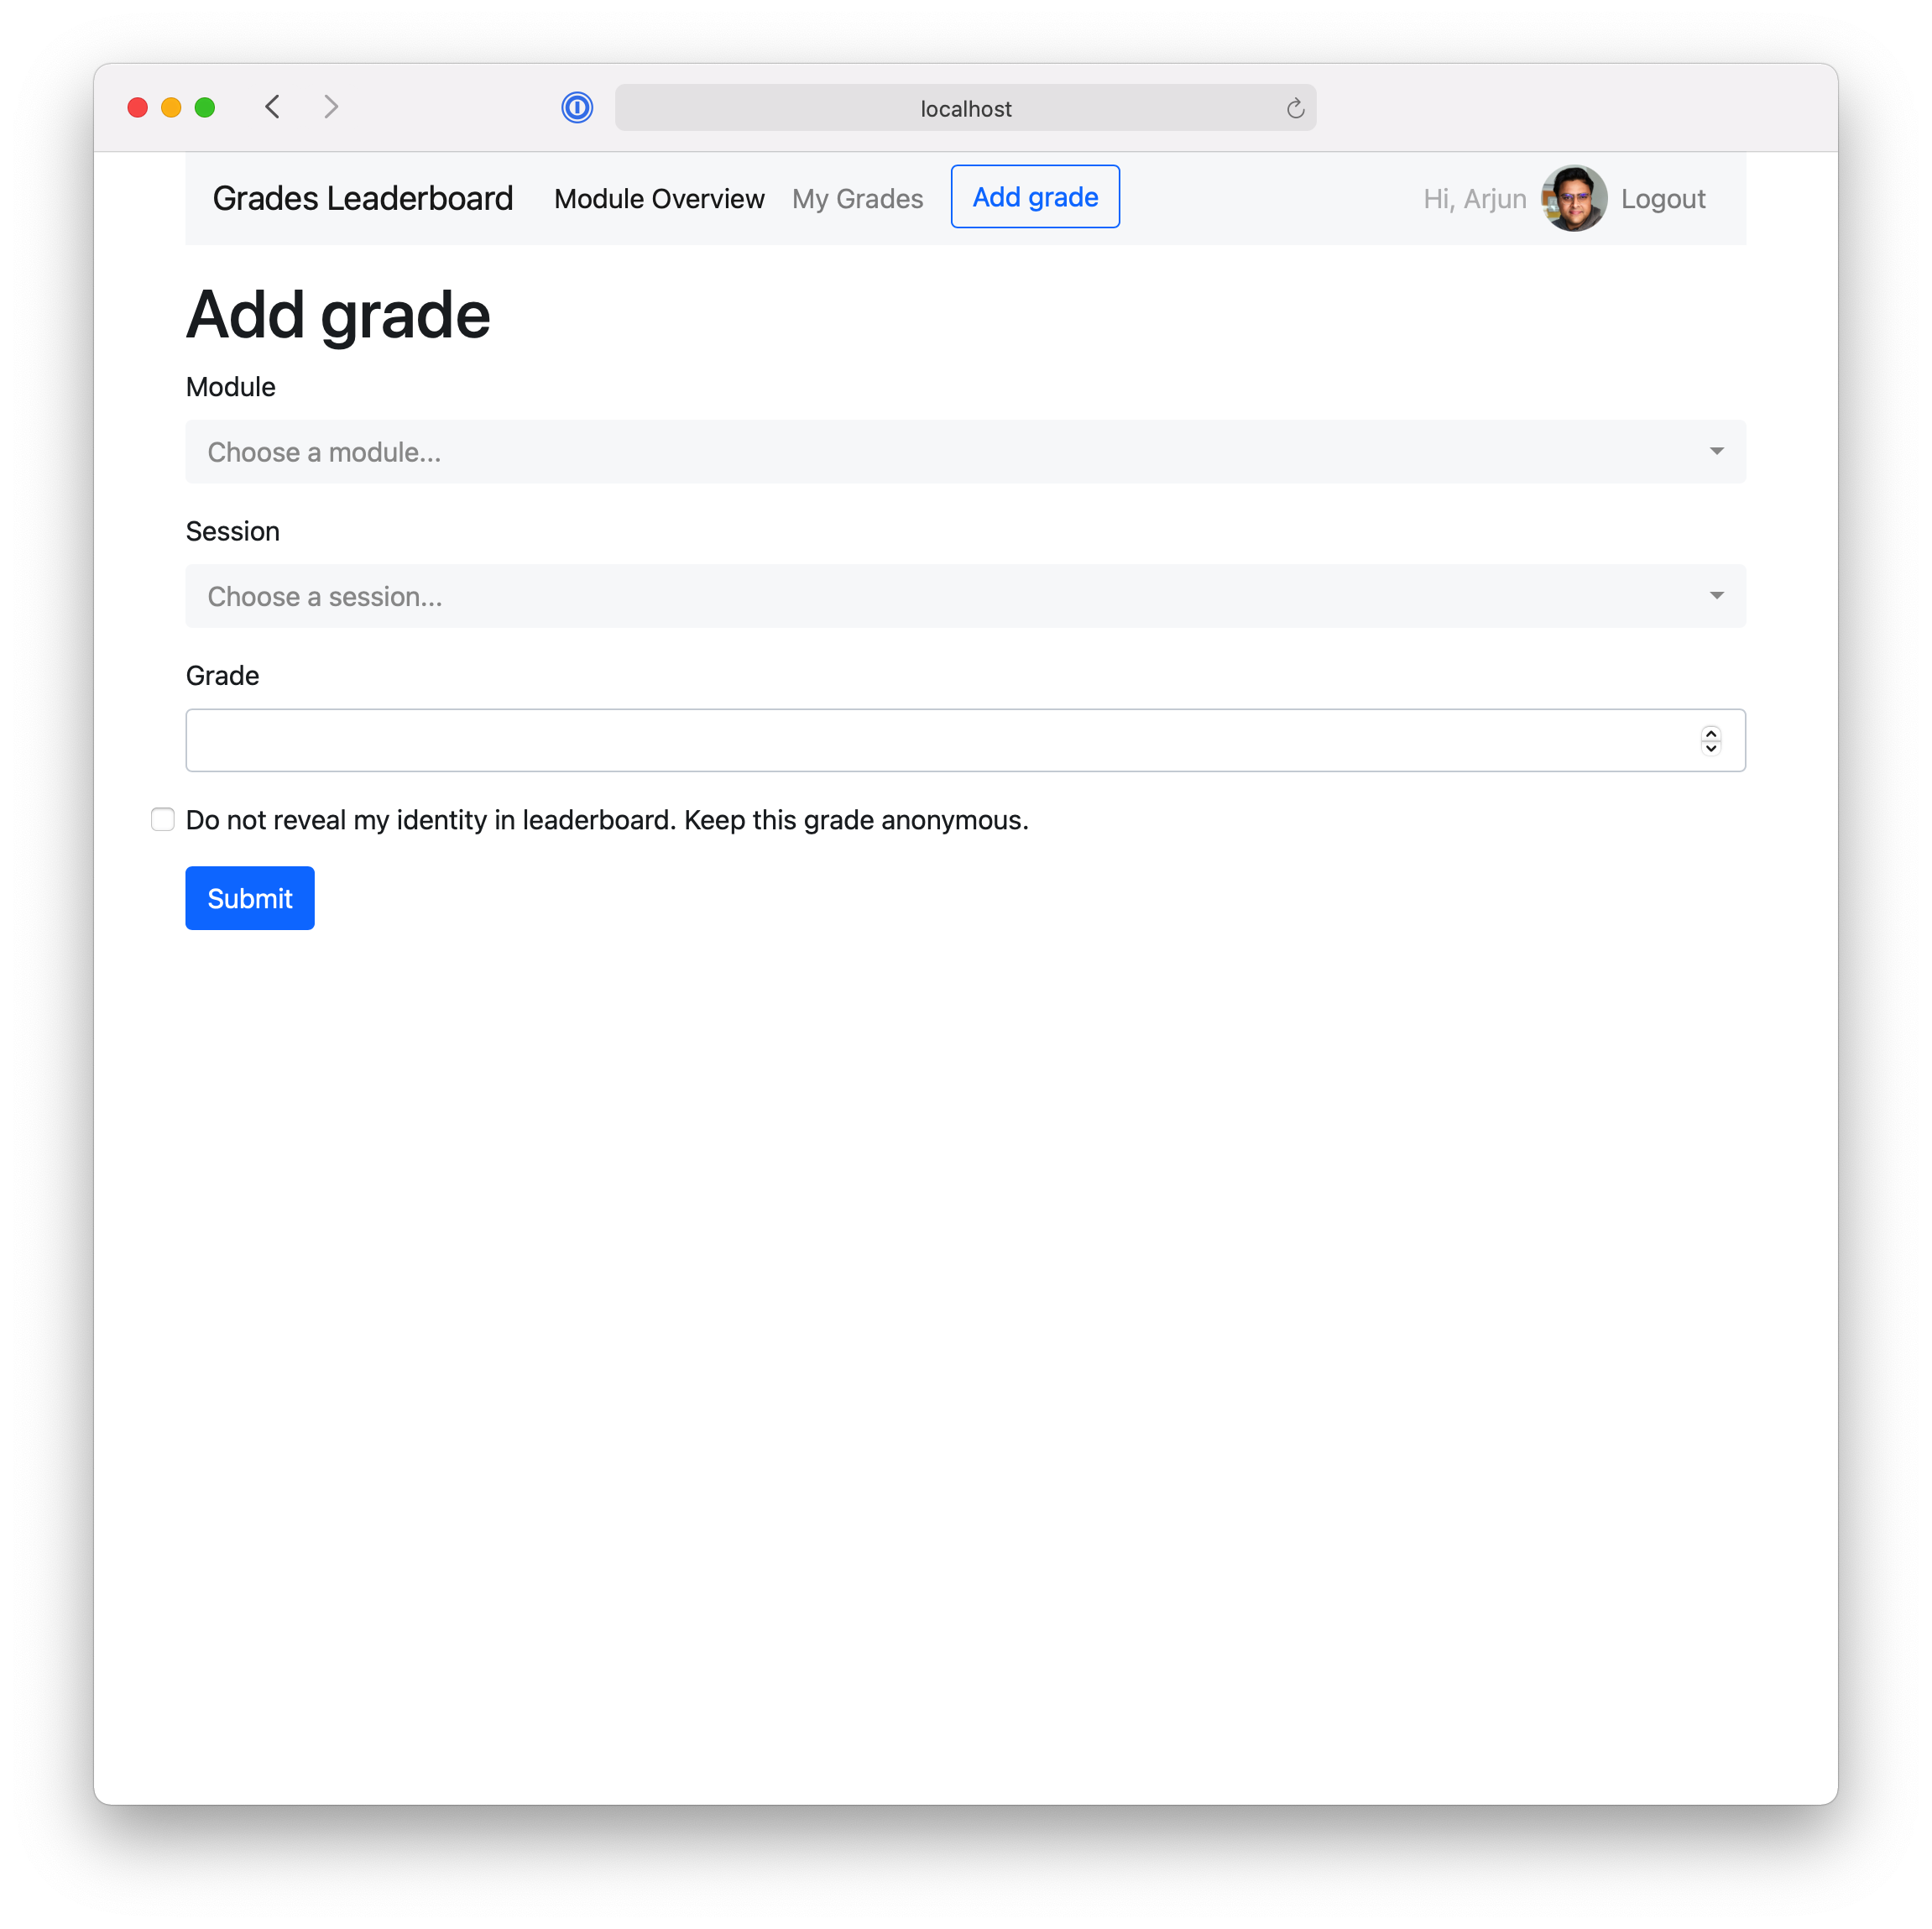
\includegraphics[width=10cm]{images/addgrade.png}
    \caption{Adding Grades}
    \label{fig:addgrade}
\end{figure}



\subsection{Cycle 2 (Sprints 4-6)}




\subsection{Cycle 3 (Sprints 7 - 9)}


\section{Analysis and Evaluation}
In order to evaluate our progress and success, we decided to select specific success factors that would indicate if the product is successful following a real-world market launch. We therefore set ourselves targets for each of these factors for both a "P0" launch, which is what we intend to build as part of this course module, and long-term goals, which are longer-term goals if this product were launched in real-world conditions.

\subsection{Critical Success Factors}
Through a further brainstorming exercise, combined with some research, we identified the following success factors.

\begin{itemize}
    \item \textbf{Reach:} The number of distinct students from the overall student population that has submitted grades. The population is defined as the number of students we can observe in the \texttt{\#general} channel of the student Slack. 
    \item \textbf{Coverage:} The number of modules that have a sufficient number of grades submitted for meaningful comparison. We define "meaningful" as a minimum of 5 grade submissions for a single module.
    \item \textbf{Repeat:} The number of students who submitted at least two grades in two distinct terms.
    \item \textbf{Adoption:} The number of academic institutions and their respective student bodies that have adopted this product.
   \item \textbf{Rating:} The average of all user-ratings in app stores where the product is available.
   \item \textbf{Usability:} Usability score measured with UMUX-Lite method
   \item \textbf{Usefulness:} Usefulness score measured with UMUX-Lite method
\end{itemize}

\subsection{Measurement of Success \& Failure}
As noted, we set ourselves targets for the initial launch as well as longer-term goals.

% Please add the following required packages to your document preamble:
% \usepackage{booktabs}
\begin{table}[H]
\centering
\begin{tabular}{@{}lcc@{}}
\toprule
                  & \multicolumn{1}{l}{\textbf{P0 Target}} & \multicolumn{1}{l}{\textbf{Long Term Target}} \\ \midrule
\textbf{Reach}    & 2\%                                   & 10\%                                         \\
\textbf{Coverage} & 20\%                                  & 100\%                                        \\
\textbf{Repeat}   & n/a                                   & 20\%                                         \\
\textbf{Adoption} & 1                                     & 20                                           \\
\textbf{Rating}   & n/a                                   & 4.5                                          \\ 
\textbf{Usability}   & 40\%                                   & 60\%                                          \\ 
\textbf{Usefulness}   & 40\%                                 & 60\%                                          \\ \bottomrule

\end{tabular}
\end{table}

\subsection{UI Evaluation}\label{sec:uieval}


\subsection{Accessibility Audit}\label{sec:access}


\subsection{User Safety \& Security}\label{sec:usersafety}


\section{Individual Reflection}


\newpage
\bibliographystyle{IEEEtran}
\bibliography{bib} 


\appendix
\appendixpage
\addappheadtotoc

\section{User Guide}\label{sec:guide}

\subsection{Slack sign-in}\label{sec:slacksignin}
\begin{figure}[H]
    \centering
    
\includegraphics[width=15cm]{images/user-guide/slack-sign-in/1.jpg}
    \caption{To sign in as a validated student, click the "Sign in with Slack" button under the "Kickstart your study motivation" card in the homepage. There is more information available by clicking on the info icon in the upper-right of the card, which is depicted in \cref{fig:slacksignin1a}}
    \label{fig:slacksignin1}
\end{figure}
\begin{figure}[H]
    \centering
    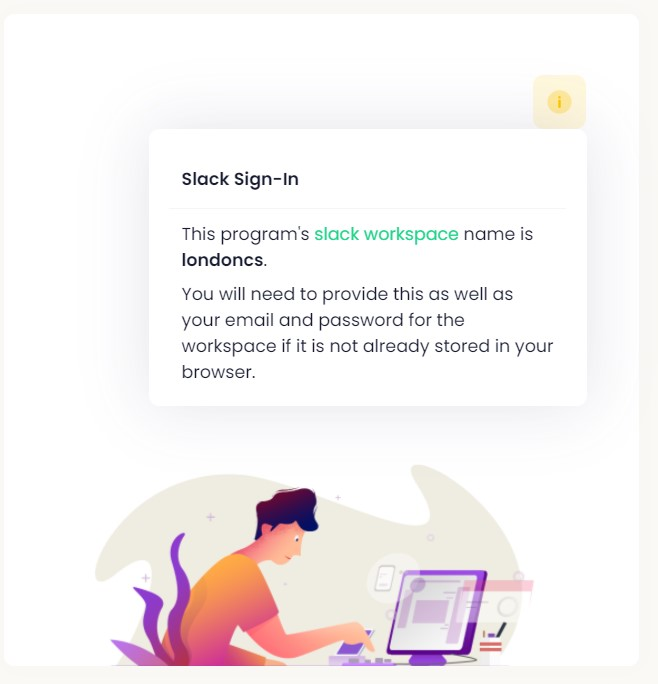
\includegraphics[width=10cm]{images/user-guide/slack-sign-in/1a.jpg}
    \caption{This information box explains what credentials you need to provide in the event that they are not saved in your browser. Slack saves these credentials in your browser by default. Typically you do not need to provide this information. If your information is saved you will be directed to the screen in \cref{fig:slacksignin4}, otherwise you will need to start the input more information as shown in \cref{fig:slacksignin2} and \cref{fig:slacksignin3}}
    \label{fig:slacksignin1a}
\end{figure}
\begin{figure}[H]
    \centering
    
\includegraphics[width=10cm]{images/user-guide/slack-sign-in/2.jpg}
    \caption{If slack credentials are not saved in your browser, enter 'londoncs' as the slack workspace and click "Continue"}
    \label{fig:slacksignin2}
\end{figure}
\begin{figure}[H]
    \centering
    
\includegraphics[width=10cm]{images/user-guide/slack-sign-in/3.jpg}
    \caption{Enter the email address associated with your londoncs slack account and slack password and click "Sign in"}
    \label{fig:slacksignin3}
\end{figure}
\begin{figure}[H]
    \centering
    
\includegraphics[width=10cm]{images/user-guide/slack-sign-in/4.jpg}
    \caption{Click "Allow" to authenticate and sign in with Slack. This is all the input required if Slack credentials are saved in your browser. You will be redirected to Gradez.}
    \label{fig:slacksignin4}
\end{figure}
\begin{figure}[H]
    \centering
    
\includegraphics[width=15cm]{images/user-guide/slack-sign-in/5.jpg}
    \caption{You are now signed in and can see your slack avatar in the upper-right of the navigation bar.}
    \label{fig:slacksignin5}
\end{figure}

\subsection{Demo sign-in}\label{sec:demosignin}
\begin{figure}[H]
    \centering
    
\includegraphics[width=15cm]{images/user-guide/demo-sign-in/1.jpg}
    \caption{To use the application without a slack account, you can use the Demo sign in feature. To sign in as the demo user, click "Demo Sign-in" in the navigation bar at the top of the page}
    \label{fig:demosignin1}
\end{figure}

\begin{figure}[H]
    \centering
    
\includegraphics[width=15cm]{images/user-guide/demo-sign-in/2.jpg}
    \caption{This will return you to the homepage signed in as the demo user, indicated by the avatar in the upper-right of the navigation bar. You can now use the application as if you were a student validated via the slack workspace.}
    \label{fig:demosignin2}
\end{figure}

\subsection{Add grade}\label{sec:addgrade}

\begin{figure}[H]
    \centering
    
\includegraphics[width=10cm]{images/user-guide/add-grade/1.jpg}
    \caption{Click "Add Grade" in the navigation bar to access the Add Grade form. Select a course and a study session. Courses that you have already submitted grades for are excluded. Click "Next Step" to continue.}
    \label{fig:addgrade1}
\end{figure}

\begin{figure}[H]
    \centering
    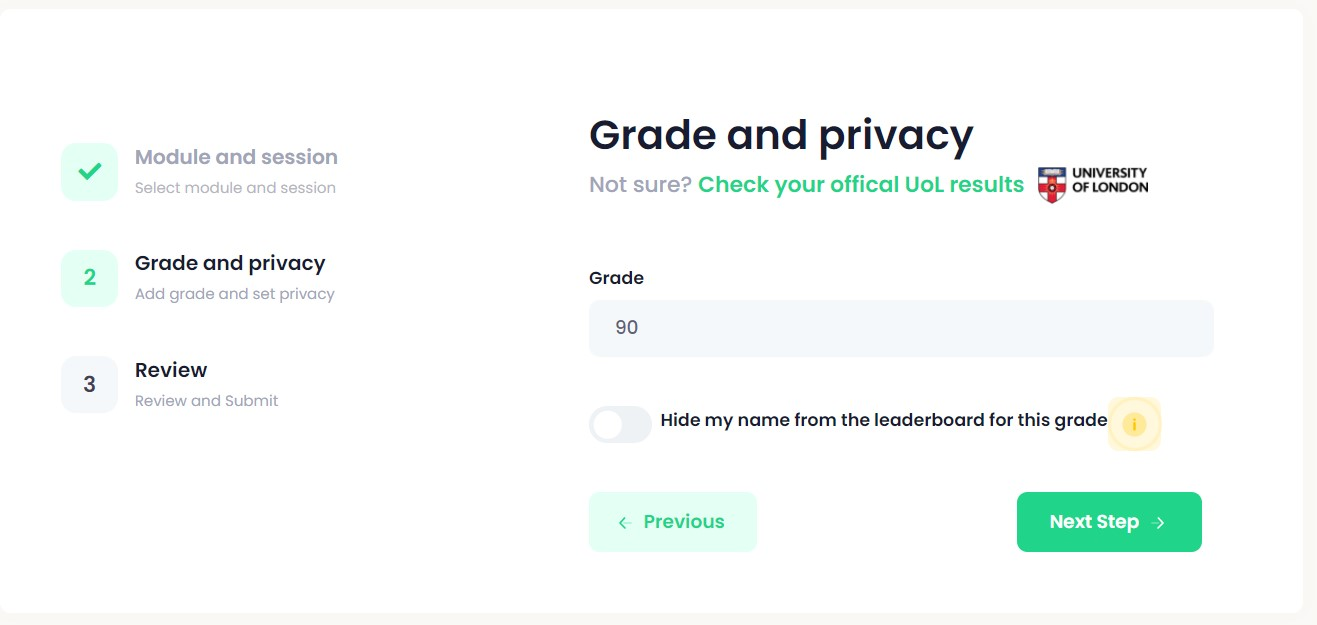
\includegraphics[width=10cm]{images/user-guide/add-grade/2.jpg}
    \caption{Enter the grade and whether or not you want to keep this grade anonymous. Click the info icon for more information on the anonymity feature. Click "Next Step" to continue.}
    \label{fig:addgrade1}
\end{figure}

\begin{figure}[H]
    \centering
    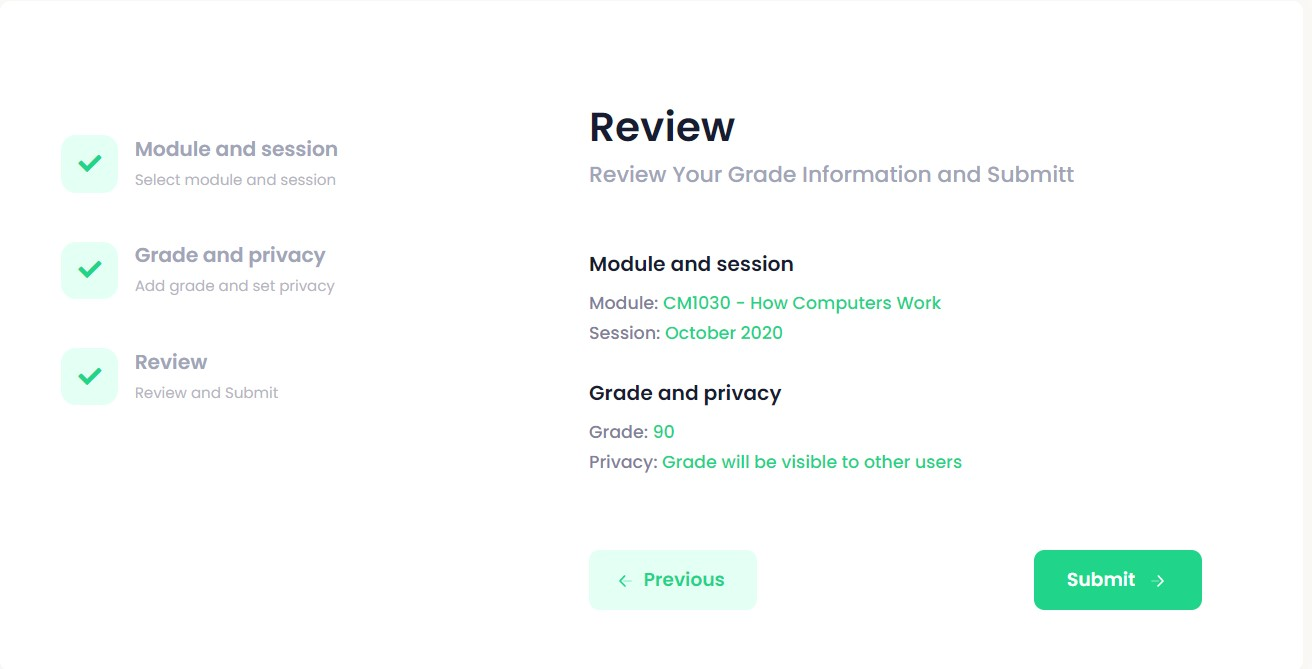
\includegraphics[width=10cm]{images/user-guide/add-grade/3.jpg}
    \caption{Review the information you provided and click "Submit" to add the grade. You can validate this submission in "My Grades" or entering the leaderboard for the course you submitted a grade for.}
    \label{fig:addgrade1}
\end{figure}

\subsection{Edit grade}\label{sec:editgrade}

\begin{figure}[H]
    \centering
    
\includegraphics[width=15cm]{images/user-guide/edit-grade/1.jpg}
    \caption{Click "My Grades" in the navigation bar to access your grades. Here you can click "Edit" next to grades as depicted above for "Intro to Programming I" to bring up the edit form.}
    \label{fig:editgrade1}
\end{figure}

\begin{figure}[H]
    \centering
    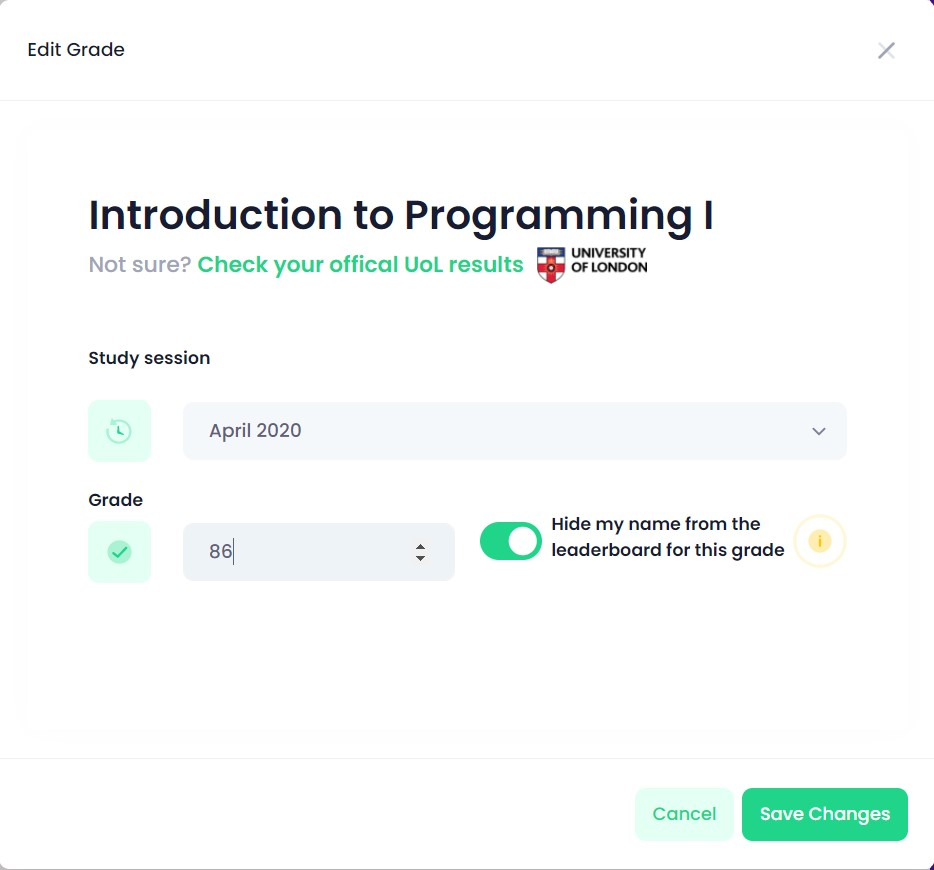
\includegraphics[width=10cm]{images/user-guide/edit-grade/2.jpg}
    \caption{Here you can change the study session, grade, and anonymity for the course. Grades are only editable for 6 months after their original submission. In this example we are changing the Intro to Programming I grade from 55, as shown in \cref{fig:editgrade1}, to 86. Click "Submit" to finish editing.}
    \label{fig:editgrade2}
\end{figure}

\begin{figure}[H]
    \centering
    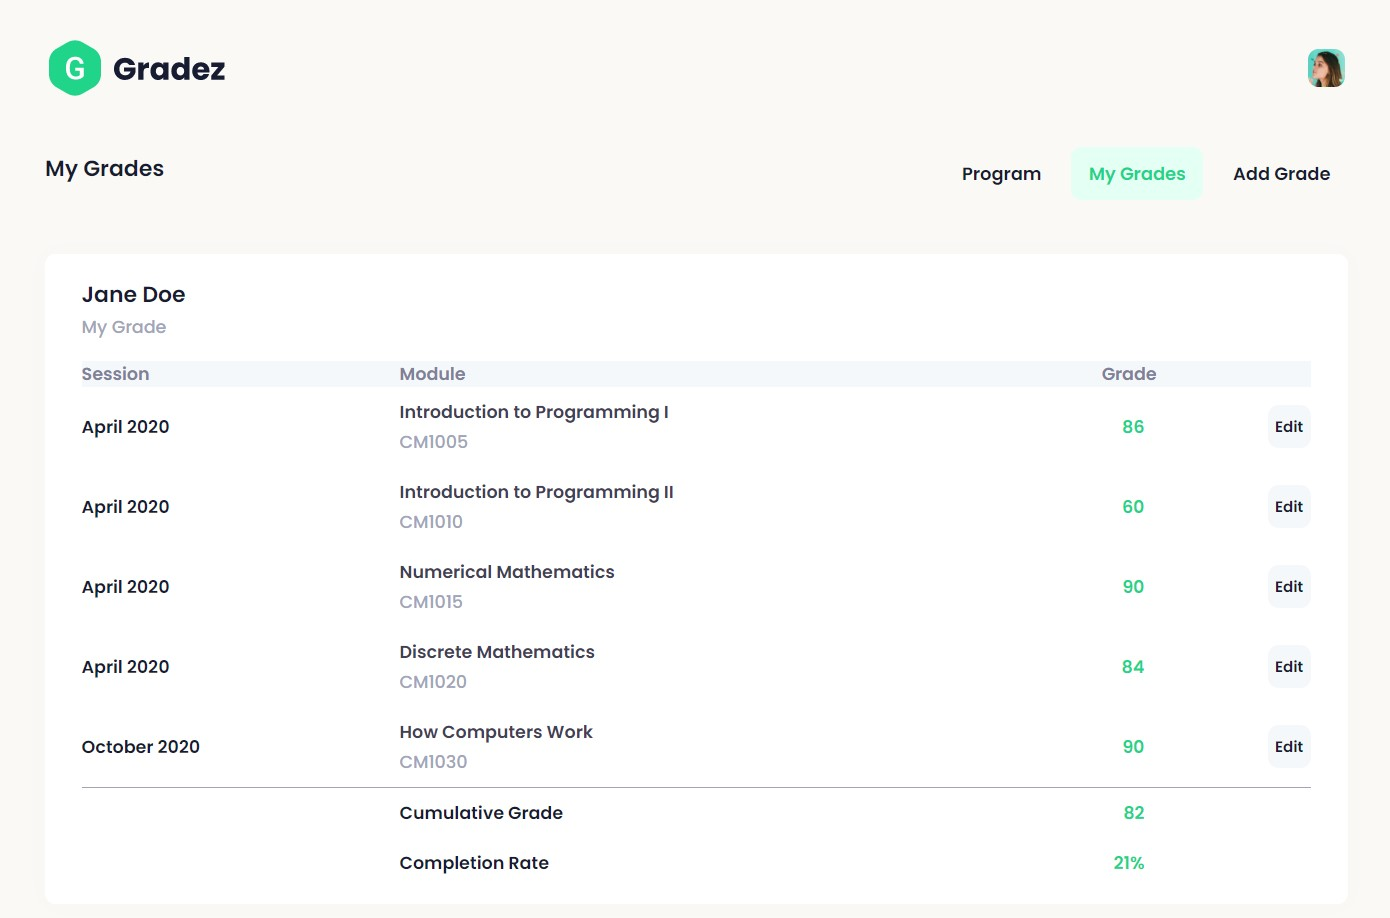
\includegraphics[width=15cm]{images/user-guide/edit-grade/3.jpg}
    \caption{Your updated information will be shown in "My Grades", as shown above, as well as the leaderboard for the class.}
    \label{fig:editgrade3}
\end{figure}

\section{User Stories}

\section{User Feedback}


\section{Git History}
The following output shows a log of work done on this assignment as it was committed to our private Git repository. This is generated by \texttt{git log --color --graph --oneline}.

\begin{minted}[breaklines]{text}
* 100bc1c (HEAD -> main, origin/main, origin/HEAD) Final version midterm
* 35c8b91 Added compelled pdf after last revision
* c8aae6f Added citations for section 1
* 1f9f666 Added citations and usability evaluation
* f296c91 Updated with compiled PDF
* fddbd84 Added more detail to initial epics - final candidate 2
* 0d49a0a Midterm final candidate
* 60b1a21 added some wireframes to section 5
* 94e4e7f Updated midterm section 6
* 48b7b4a updated wireframes
* feeeaa5 Update leaderboard_wireframes.bmpr
* 8f28ebb added the rest of 12-21 notes
* 0d09fae added my meeting notes
* 354fc35 new revision from group session
* 0cf3b52 updated overleaf as images were not visible or outdated
* 62ca2e7 new wireframes, renamed source file
* 5995e79 Added framing to SWOT/STEEPLE and added author names.
* 1a29062 Reviewed and restructured midterm LaTeX file. Edited sections 2-5 and created tables. Incorporated storyboard graphics.
* f4465f9 Create casual_checker_1.png
* de57acb Create competitive_topper_1.png
* b32c653 export of gantt used in proposal
* 41852f6 Some rough ideas for reports to the user
* b7dea47 Modified wireframe
* 9f86020 Added account log in and sign in pages
* 54bf1e4 initial attempt at wireframe prototype
* 1f79184 Amended minutes
* 39db9d6 Minutes from 2020-12-10 session
* 04fa4e1 Notes 2020-12-07
* 1dc2d5b added updated midterm report pdf
*   5f165af Merge branch 'main' of https://github.com/BlairCurrey/uol-agile-group-project into main
|\
| * f35e4a3 Added a couple of comments on the meeting
| * d70fb30 Fix date
| *   c2d0c6a Merge branch 'main' of https://github.com/BlairCurrey/uol-agile-group-project into main
| |\
| | * 273900f Updated notes 3-Dec-2020
| | * 0f60790 Uploaded summary of the book
| * | 03b91ca Capture ideation board after the meeting
| |/
| * abaac74 Update TG1_G6_GroupMeetings.md
| * a2e19a4 Updating exports of Miro
* | 51d1a3a Add STEEPLE & changed market analysis sectioning
|/
* 6424a17 added methodology for gathering competitors
* 1022228 images for market research
* e358d8f added Market Research
* 03e7384 Setup agenda for next meeting
* 0e21f30 Updated notes 27-11-2020
* effc3bd Added Tex Template for Midterm
* 23a65f7 Updated meeting outcomes November 23
* 29ab345 Update TG1_G6_GroupMeetings.md
* 347db17 2020-11-19 check-in
* 4f45b8a added 2020-11-12 meeting
* 7556267 corrected date for second meeting
* 859b63f Documentation for Weekly Working Session 2020-11-09
* 9b7188d Added Meeting Notes 2020-11-05 and updated README
* f461ecf Initial commit
\end{minted}

\end{document}
